% Sample Dissertation, Thesis, or Document %
%            for use with the              %
%  University of Arizona Thesis Class,     %
%               uathesis.cls               %
%------------------------------------------%

% We'll use the uathesis document class (duh).  The uncommented line
% below will produce a Dissertation, the others would produce a Thesis
% or a Document.  There are other options available to you like turning
% on the copyright statement and replacing the year on the title page
% with a "generated on" stamp (handy for early drafts).  To find out
% what the available options are, take a look into the uathesis.cls
% file and look for the \DeclareOption commands near the top of that
% file.
% There are five copyright options.  Copyright, no copyright, and three
% different Creative Commons licences.  Use the one you want (If you go
% Creative Commons, I (DM) think the CC-BY-ND makes the most sense)  See
% uathesis.cls for the reason why the non-commercial licenses are not
% included.
\documentclass[dissertation]{uathesis}
%\documentclass[dissertation,copyright]{uathesis}
%\documentclass[dissertation,CC-BY]{uathesis}
%\documentclass[dissertation,CC-BY-SA]{uathesis}
%\documentclass[dissertation,CC-BY-ND]{uathesis}
%\documentclass[thesis]{uathesis}
%\documentclass[document]{uathesis}

% Package Usage
% These are the packages that we need
\usepackage{graphicx}
\usepackage{natbib}			% natbib is available on most systems, and is
					% terribly handy.
					% If you want to use a different Bibliography package, 
					% you should be able to, just change this
					% and the \bibliographystyle command below.  Be warned
					% that you may need to do a little hacking to get
					% the REFERENCES item to show up in your TOC.

% Compatibility with the AASTEX package 
% of the American Astronomical Society.
% I COMMENTED OUT LINE 150 OF DELUXETABLE.STY
\usepackage{deluxetable}		% Allows use of AASTEX deluxe tables
\usepackage{aastex_hack}		% Allows other AASTEX functionality.
\usepackage{nicefrac}

% These are other packages that you might find useful.
% For controlling the fonts, see
% http://www.math.uiuc.edu/~hartke/computer/latex/survey/survey.html
% The following is a nice font set:
%\usepackage{mathtime}			% Times for letters; Belleek math.
%
\usepackage{amsmath}			% AMS Math (advanced math typesetting)
\usepackage{amssymb} 
\usepackage{lscape}			% Used for making fitting large tables in by putting them landscape
\usepackage[tableposition=t]{caption} % NICK ADDED THIS (makes table captions normal size when font set smaller)

%%% Evan added the following
\usepackage{mathtools}
\usepackage{bm}
\usepackage{enumitem}
\usepackage{units} % includes nicefrac

%%% The following allows dagger footnote on chapter titles
%%% with no number. Useful for designating previously 
%%% published work.
\newcounter{daggerfootnote}
\newcommand*{\daggerfootnote}[1]{%
    \setcounter{daggerfootnote}{\value{footnote}}%
    \renewcommand*{\thefootnote}{\fnsymbol{footnote}}%
    \footnote[2]{#1}%
    \setcounter{footnote}{\value{daggerfootnote}}%
    \renewcommand*{\thefootnote}{\arabic{footnote}}%
    }

\newcommand{\Msun}{\mathrm{M}_{\odot}}
%\usepackage{refs}			
%
% If you are using hyper-ref (recommended), this command must go after all 
% other package inclusions (from the hyperref package documentation).
% The purpose of hyperref is to make the PDF created extensively
% cross-referenced.
\usepackage[hidelinks]{hyperref}

% Set up some values.
\completetitle{Magnetic Reconnection in Low-Luminosity Accretion Flows: from Microphysical Simulations to Large-Scale Models}
\fullname{David Ramsey Ball}			% Grad college wants your full name here.
\degreename{Doctor of Philosophy}	% Title of your degree.
\degreemajor{Astronomy and Astrophysics} % Degree major
\begin{document}


% Set up the title page
\maketitlepage
{University of Arizona Department of Astronomy}	% Title of your department.
{2020}							

% Insert the approval form.  Note that for electronic submission
% of your Ph. D. dissertation, you must bring *two* copies of the
% approval page to your final defense.  These must be signed by
% the committee.  Make two photocopies: one for Pam and the other
% for your records.  Then, bring the two signed originals to the
% graduate college when you submit the final version of the
% dissertation to the University of Arizona.
\approval
{}		% Defense Date	
{}	% Dissertation Director
{}	% 1st committee member
{}		% 2nd committee member
{}		% 3rd committee member
{}		% 4th committee member
{}		% 5th committee member
{}		% 6th committee member

% Include the ``Statement by Author'' for Dissertations
\statementbyauthor
% If this is a Thesis, use the following form, with your thesis director's
% name and title in the square brackets like so (you should also omit the 
% approval form insertion above):
%\statementbyauthor[Jane M. Doe\\Professor of Chemistry]

% Include the ``Acknowledgements''
\incacknowledgements{acknowledgements}

% Include the ``Dedication''
\incdedication{dedication}

% Create a ``Table of Contents''
\tableofcontents

% Create a ``List of Figures''
%\listoffigures

% Create a ``List of Tables''
%\listoftables

% Include the ``Abstract''
\incabstract{abstract}

% Include the various chapters
\chapter[Introduction]
{Introduction}
%\begin{figure}
%\centering
%\includegraphics[angle=0,width=\columnwidth]{fig1.pdf}
%\caption[]{}
%\label{fig1}
%\end{figure}
\section{Black Holes and Accretion}

Black holes have drawn substantial attention from both scientists and the public since Karl Schwarzchild first formulated them as a solution to Einstein's field equations (\citealt{schwarzschild1916}).  Since then, scientists have generated a massive body of work focused on understanding these captivating objects and the material that collects around them.  In this dissertation, we will focus on understanding the physics of hot ionized gas (or, plasma) that swirls around black holes and heats up to extremely high temperatures, lighting up the direct surroundings of black holes at nearly all wavelengths, from the radio to X-ray.  

Black holes range in size, from just over the mass of the Sun ($3.8 M_{\rm{sun}}$, \citealt{smallbh}), to over a billion times the mass of the Sun ($6.5\times10^9 M_{\rm{sun}}$, e.g., \citealt{eht6}).  We will focus on so-called ``supermassive black holes" (defined for our purposes as $M>10^6 M_{\rm{sun}}$).  Supermassive black holes can have profound impacts on their environments and are responsible for a variety of critical phenomena in terms of galaxy evolution.  For instance, the supermassive black hole at the center of M87 is thought to be responsible for generating powerful jets that we see emerging from a very compact source in this galaxy (reference).  More recently, this black hole was imaged by the Event Horizon Telescope collaboration (EHT) and showed the telltale sign of the ``black hole shadow'' imprinted on the surrounding material's emission.  By providing the first horizon-scale imaging of black holes, the EHT provides a new testbed not only for General Relativity, but also for our understanding of plasma physics in a regime that terrestrial experiments cannot probe.

The closest supermassive black hole to the Earth is Sagittarius A* (henceforth Sgr~A*), which resides at the center of our own Milky Way galaxy.  Numerous observing campaigns have been dedicated to characterizing the emission from this source, both in terms of its spectrum, as well as its variability (references).  These detailed observations, when combined with the appropriate physical models, are extremely powerful in furthering our understanding of the physics of these systems.  Sgr~A* is quite dim, and hence, is classified as a ``low-luminosity accretion flow'', and is thought to have a very low accretion rate $\sim 3 \times 10^{-5} \; \rm{M_{sun}} \; \rm{yr}^{-1}$ (e.g. \citealt{quataert1999b}).  We will elaborate further on the physics of low-luminosity accretion flows in section \ref{sec_lowlum}.

Observations of Sgr~A* reveal significant multiwavelength variability (see \citealt{eckart2004, marrone2008, neilsen2013, witzel2013, ponti2015, li2015, wang2016}) from the mm and IR to the X-rays.  At high energies, in particular, \citet{neilsen2013} analyzed 3 million seconds of Chandra data dedicated to characterizing both short and long-term X-ray variability of Sgr~A*.  They found that the length of flares varies from a few hundred seconds to 8 ks, with luminosities from $\sim 10^{34} \; \rm{erg} \; \rm{s}^{-1}$ to $2 \times 10^{35} \; \rm{erg} \;  \rm{s}^{-1}$.  More recently, \citet{haggard2019} quantified the behavior of some of the brightest X-ray flares, and showed that some of them have distinct double-peaked structures to the lightcurve.  \citet{eckart2004} carried out simultaneous observations in both the X-ray and near IR, and found that X-ray flares always have a coincident IR flare.  In contrast, there are numerous IR flares without X-ray counterparts.  These flares can offer unique insight into the particle energetics of the accretion flow; highly energetic stochastic flares point towards mechanisms such as shocks and magnetic reconnection, which are capable of quickly producing large numbers of high energy non-thermal particles which significantly alter the observational signatures of the accretion flow.

\section{Low-Luminosity Accretion Flows}
Many supermassive black holes, including Sgr~A*, have small accretion rates, and as a result, have very low luminosities.  In these systems, the radiative efficiency is low due to the low density of the plasma in the flow, and hence are often coined ``radiatively inefficient accretion flows'' (henceforth, RIAFs).  In contrast with relatively cold and radiatively efficient thin disk models, radiatively inefficient accretion flows remain very hot precisely because the energy carried away by radiation is negligible compared to the viscously dissipated energy in the system.  The high temperatures and low densities in these disks cause them to be geometrically thick and optically thin.  As such, their spectra are dominated by various emission processes such as synchrotron and bremsstrahlung that occur at different locations throughout the disk, resulting in spectra that deviate substantially from a simple blackbody.

The low plasma density in RIAFs has a number of interesting implications.  The timescale for electron-ion Coulomb collisions to exchange energy is longer than the heating timescale, which means that the electrons and ions likely have different temperatures.  Electrons are expected to be substantially colder than ions for a number of reasons: first, heating mechanisms such as the dissipation of turbulent (or magnetic) energy and shocks tend to favor the more massive species (\citealt{howes2010}, \citealt{rowan2017}) across a broad range of plasma parameters (with the exception of when the plasma-$\beta$, the ratio of gas to magnetic pressure, is very low), second, electrons radiate away their energy at a much faster rate than ions.  In addition to ions and electrons being thermally decoupled, electron-electron and ion-ion Coulomb collision timescales are also  longer than dynamical timescales, meaning the distribution function of each species may be highly nonthermal (i.e., deviating substantially from a Maxwellian).

The role of non-thermal electron energy distributions have been addressed in the context of stationary hydrodynamic models by \citet{mahadevan1998}, \citet{ozel2000}, and \citet{yuan2003}, who showed that even a relatively small number of power-law electrons can significantly impact the spectra predicted from a model, generating X-ray power-law tails as well as boosting the low frequency radio flux.  These studies used analytical steady-state solutions to calculate spectra, which do not capture short timescale GRMHD effects that play a large role in determining the variability properties of the system.  In section \ref{phenom_model}, we will elaborate further on the work that has been done to address nonthermal electrons in low-luminosity accretion flows, and describe a phenomenological model we developed to explain the X-ray flares from Sgr~A* in the framework of magnetohydrodynamic simulations and radiative transfer calculations.

\label{sec_lowlum}
\section{Magnetohydrodynamics}
While substantial work has been done to analytically understand the steady-state global solutions to RIAFs (see \citealt{yuan2014} for a recent review), these calculations make a number of simplifying assumptions.  In particular, in order to make the calculations tractable, most studies assume steady and axisymmetric accretion flows and also prescribe an artificial kinematic viscosity to enable accretion.  While these solutions are enlightening and highlight some of the basic underlying physics of accretion disks, they are not suited for studying the nonlinear physics of accretion, the turbulence that arises, and the associated variability in emission.  In order to understand these processes, we must turn to numerical simulations.

The most commonly used type of simulation to study accretion flows around black holes are ``general relativistic magnetohydrodynamic'' (henceforth GRMHD) simulations.  In short, these are simulations that capture the dynamics and energetics of an ionized gas in the static but curved spacetime around a black hole.  The framework of MHD makes a number of simplifying assumptions.  First, it assumes that the plasma satisfies the fluid approximation: that the collisional mean-free-path is much less than the scale of interest.  Most MHD simulations also utilize the ``ideal MHD'' approximation: that the plasma is infinitely conductive.  In other words, because electrons have such a small mass, they respond extremely rapidly to the presence of electric fields and will immediately short out any electric field in the system, ensuring that the fluid remains electrically neutral.  One consequence of the ideal MHD approximation is that it effectively ``freezes'' the magnetic field into the fluid, so that the evolution of the magnetic field is simply described as being advected around with the fluid.  In reality, the ideal MHD approximation drops a number of other higher-order terms to simplify the evolution of the magnetic field, we will now briefly cover how the evolution of the magnetic field evolves in the framework of ideal MHD and the assumptions used to get there.  For clarity, all of the following equations in this section are in the nonrelativistic limit, where the equations lend themselves far more readily toward building physical intuition.  We note, however, that the general principles we discuss also apply to the relativistic analogs.

We will begin by considering the generalized Ohm's law:

\begin{equation}
	\bold{E}+\bold{u}\times \bold{B} = 
	\eta \bold{J} + \frac{1}{e n}\left(\bold{J} \times \bold{B} - \nabla \cdot \overleftrightarrow{\bold{P}}_{e} + \frac{m_e}{e}\left[\frac{\partial \bold{J}}{\partial t}+\nabla \cdot (\bold{Ju} + \bold{uJ})\right]\right).
	\label{ohm}
\end{equation}

Here $\bold{E}$, $\bold{B}$, $\bold{u}$, and $\bold{J}$ represent the electric field, magnetic field, fluid velocity (the mass-weighted average velocity, including both species), and current, while $\overleftrightarrow{P_e}$ represents the electron pressure tensor.  In this dissertation, bolded quantities represent vectors while double arrows above a bold quantity represent rank-2 tensors.  The remaining quantities: $\eta$, $e$, $n$, and $m_e$ are simply the fluid's resistivity, the charge of a proton, the number density of the fluid, and electron mass.  In this equation, the first term on the right hand side is simply Ohmic dissipation. The first term in parenthesis is the so-called ``Hall'' term and the following two terms include effects from the divergence of the electron pressure tensor and electron inertial effects, all of which contribute to the electric field.  For most purposes, the terms within the parenthesis are neglected due to the small factor of $1/en$, which is typically negligible compared to the other terms in the equation in astrophysical contexts.  The ideal approximation sets the entire right hand side to 0 (by the argument that $1/en$ is very small, and that the electrical resistivity, $\eta$, is nearly 0, corresponding to an infinite conductivity $\sigma=1/\eta$).  This results in the much simpler expression for the electric field of

\begin{equation}
	\bold{E}_{\rm{ideal}}=-\bold{u}\times \bold{B}.
	\label{ideal_E}
\end{equation} 

This electric field is often referred to as the ``ideal'' or ``motional'' electric field, and can be understood simply as the electric field induced by moving magnetic fields.  In order to assess the evolution of the magnetic field, we plug the electric field found in \ref{ideal_E} into Faraday's law:

\begin{equation}
	\frac{1}{c}\frac{\partial \bold{B}}{\partial t} = - \nabla \times \bold{E_{\rm{ideal}}}=\nabla \times (\bold{u}\times\bold{B})
	\label{faraday}
\end{equation}

This leads to a phenomenon known as ``flux freezing'': it is relatively straightforward to show that Equation \ref{faraday} implies that the magnetic flux through a fluid element is conserved as the fluid moves.  Another related, although not identical implication is the so-called ``Lundquist Theorem'' that shows that Equation \ref{faraday} more generally describes how a any vector field (in this case, $\bold{B}$) is advected by a velocity field.  This means that the magnetic field can be stretched and compressed by fluid motions, but cannot reconnect or dissipate.

The underlying assumptions that lead to the equations of ideal MHD make the system of equations much more tractable to implement numerically.  Furthermore, the assumptions are quite sound for a large number of astrophysical systems and scales.  MHD (and GRMHD, when necessary) has proven to be a powerful tool over the last few decades and has explained a wide variety of astrophysical phenomena, from accretion on to black holes, to the behavior of plasma in the outskirts of galaxy clusters, to the solar wind and corona.

\subsection{Shortcomings of the MHD approximations}
While the fundamental assumptions of ideal MHD may be valid on the largest scales in the system, in principle, small regions may arise that violate the underlying assumptions.  For instance, if we consider the generalized Ohm's law (Equation \ref{ohm}) in the limit where the Hall, electron pressure tensor, and electron inertia terms are negligible, we get the ``resistive Ohm's law'',

\begin{equation}
\bold{E} + \bold{u} \times \bold{B} = \eta \bold{J}.
\end{equation}

In order to assess the importance of a finite resistivity on the evolution of the magnetic field, we once again plug the electric field into Faraday's law:


\begin{equation}
	\frac{1}{c}\frac{\partial \bold{B}}{\partial t} =\nabla \times (\bold{u}\times\bold{B}) -\nabla \times \eta \bold{J}
	\label{faraday_resistive}
\end{equation}
	
In the limit of nonrelativistic MHD, the current is simply the curl of the magnetic field, i.e.,

\begin{equation}
	\bold{J} = \frac{c}{4\pi}\nabla \times \bold{B}.
\end{equation}
As such, we can write the evolution of the magnetic field in terms of itself and the fluid velocity as 

\begin{equation}
	\frac{1}{c}\frac{\partial \bold{B}}{\partial t} =\nabla \times (\bold{u}\times\bold{B}) -\nabla^2 \eta \bold{B}.
\end{equation}
In most cases, we assume that the resistivity is roughly constant in space so that it simply acts as a diffusion coefficient via

\begin{equation}
		\frac{1}{c}\frac{\partial \bold{B}}{\partial t} =\nabla \times (\bold{u}\times\bold{B}) -\eta \nabla^2 \bold{B}.
\end{equation}

We see that the effect of a finite resistivity serves to dissipate the magnetic field.  In the ideal MHD assumption, we dropped the resistive term, arguing that $\eta$ is small.  Here, however, we see that even in the limit where $\eta$ is small, if regions arise where $\nabla^2 \bold{B}$ is large, then the $\eta \nabla^2 \bold{B}$ term may end up being dynamically and energetically important to this system.  One such type of configuration that may arise is a so-called ``current sheet'', where the magnetic field reverses its direction over a short length scale.  This configuration is unstable and prone to undergo magnetic reconnection, which we will describe in more detail in the following section and will be a focus of this dissertation.

\section{Magnetic Reconnection}
Magnetic reconnection is a fundamental plasma process in which opposing field lines in a plasma that are separated by a short distance rearrange their topology, connecting with one another.  In doing so, they release magnetic energy into the ambient plasma in the form of bulk motion, heat, and in some cases, particle acceleration.  Reconnection was first formulated in the context of resistive MHD by Eugene Parker and Peter Sweet in 1956 in an attempt to explain the dynamics of solar flares.  We will now briefly review a dimensional argument that follows their original formulations from \citet{parker1957} and \cite{sweet1958} and is widely known as the ``Sweet-Parker'' model of reconnection.  Because this is not a rigorous derivation, but rather a scaling argument, we will not concern ourselves much with factors of order unity, but instead focus on the underlying physics and trends that this model uncovers.

Consider a current sheet in which the x-component of the magnetic field, $B_x$, reverses direction over a distance of $\delta$ in the y-direction, and extends along a distance $L$ in the x-direction.  On either side of the layer, the strength of the magnetic field is $B$.  This geometry will have an associated current in the z-direction with a magnitude of 

\begin{equation}
	J_{\rm{z}} = \frac{c}{4 \pi}\frac{B}{\delta}.
\end{equation}    

Outside of the current sheet, the magnetic field strength is constant, and hence there is no current.  As such, the only electric field in this region is from magnetized plasma flowing towards the layer (in the y-direction), which will have a magnitude of $E_{\rm{outside}} \approx u_{\rm{in}}B$, where $u_{\rm{in}}$ is the inflow speed (the bulk velocity of plasma flowing towards the current layer in the y-direction).  Within the layer, the magnetic field goes to 0, so there is no ideal electric field.  There is, however, a current and finite resistivity.  As such, there will be a resistive electric field with magnitude 

\begin{equation}
E_{\rm{inside}} \approx \frac{c}{4\pi}\frac{\eta B}{\delta}.
\end{equation}

By matching $E_{\rm{inside}}$ to $E_{\rm{outside}}$, we can derive an expression for the inflow speed as a function of the other parameters in the setup,

\begin{equation}
	u_{\rm{in}} = \frac{c}{4 \pi} \frac{\eta B^2}{\delta}.
\end{equation}

In the geometry in which plasma is flowing towards the current layer in the outer region (in the y-direction), and plasma within the current sheet flows out along the x-direction, the equation of energy conservation of energy can be written as

\begin{equation}
	\frac{B^2}{4 \pi} = \frac{1}{2}\rho u_{\rm{out}}^2.
\end{equation}

From here, we see that the outflow speed is simply the Alfv\'en speed: 

\begin{equation}
	u_{\rm{out}}=\frac{B}{\sqrt{4\pi \rho}}
\end{equation}

With a bit algebra, it is straightforward to show that the inflow speed can be written simply as $\eta/\delta$, resulting in a reconnection rate that is far too slow to account for observed astrophysical phenomena.  While the Sweet-Parker model of reconnection is quite simplified and doesn't account for some important and relevant physics, it highlights a few key properties of the geometry and dynamics of current sheets: first, a thin layer of plasma within the current sheet flows outward at the Alfv\`en speed.  Second, the upstream plasma flows in at a rate dictated by the microphysics of resistivity.  If some additional effects occur that can artificially boost the effective resistivity of the plasma in the current layer, then reconnection will speed up and can explain a wide variety of astrophysical phenomena. 

Numerous theoretical models have been developed since the Sweet-Parker model to address the slow reconnection rate of the Sweet-Parker model (see \citealt{loureiro2016} for a comprehensive review of theoretical models of reconnection).  These models vary widely, from invoking standing slow-mode shocks or background turbulence, to inferring the presence of instabilities in the current sheet that fragment it into numerous magnetic islands (plasmoids), resulting in bursty and fast reconnection, as opposed to the slow and constant reconnection in the Sweet-Parker model.  As we will see later in this dissertation, the so-called ``plasmoid'' instability (also often referred to as the tearing instability) plays a crucial role in regulating not only the reconnection rate, but also the particle acceleration properties of reconnection layers.
 

Magnetic reconnection is widely thought to play an important role in the episodic flaring activity of numerous astrophysical systems, including blazar jets (\citealt{giannios2013, petropoulou2016, nalewajko2016}), pulsar wind nebulae (\citealt{coroniti1990, lyubarsky2001, zenitani2001, kirk2003, contopoulos2007, petri2008, sironi2011, cerutti2012,cerutti2014,cerutti2017, philippov2014} see \citealt{sironi2017} for a recent review), gamma ray bursts (\citealt{thompson1994, thompson2006, usov1994, spruit2001, drenkhahn2002, lyutikov2003, giannios2008}). the Sun (\citealt{forbes1996, yokoyama2001, shibata2011}), and accretion flows around black holes (\citealt{galeev1979, dimatteo1998, uzdensky2008, li2015, ball2016, li2017}).  Through magnetic reconnection, energy stored in magnetic fields dissipates into the ambient plasma, resulting in particle heating and, in some cases, particle acceleration.  Electrons accelerated to ultra-relatvistic energies can produce flares and high-energy emission.  Many of these astrophysical systems consist of low-density ``collisionless'' plasmas, where the timescale for Coulomb collisions is significantly longer than dynamical timescales.  Here, the dynamics and energetics of magnetic reconnection can be properly captured only by means of a fully-kinetic framework, which can be achieved via numerical techniques such as particle-in-cell (PIC) simulations.


\section{Particle-in-Cell Simulations}
The Particle-in-Cell (henceforth, PIC) method is a fully kinetic framework for simulating a plasma.  In contrast to a fluid framework, where it is assumed that frequent collisions relax the distribution to an isotropic Maxwellian, the distribution function can be arbitrarily complex in kinetics.  As a concrete example of how this may affect the outcome of a simulation, imagine two electron beams with equal and opposite velocities, such that these two populations of electrons are passing through one another.  In a fluid framework where we take moments over the velocity distribution to attain an average ``fluid'' velocity, we lose information about the underlying distribution, because these two interpenetrating beams' velocities average to zero, so as a fluid, the velocity is zero.  In a kinetic framework, however, we retain the complex nature of this distribution, which it turns out in this particular example, is important to the overall dynamics: in this setup, the well-known ``Weibel'' instability will set in, generating small magnetic fields perpendicular to the direction of motion of the beams, and eventually scatter and isotropize the distribution.  In addition to not making assumptions about the distribution functions, PIC simulations do not assume anything about the conductivity, as in the case of ideal MHD.  Because of this, they are well-suited to studying the detailed physics of localized reconnection regions and to understand the particle acceleration properties therein.

PIC simulations work in the following way: we have a simulation domain with some number of particles (both ions and electrons) which have continuously varying positions and velocities.  These particles, however, live on a grid that stores the local electric and magnetic fields.  In order to advance the positions of the particles, we interpolate the the electromagnetic fields to the position of the particles and push the particles with the Lorentz force (the numerical implementation of integrating the equation of motion will be discussed later in this section).  After updating the positions of the particles, we then deposit their charges and currents on to the grid, and solve Maxwell's equations to update the electric and magnetic fields.  This process creates a self-consistent loop that makes no simplifying assumptions about the physics.  

While the PIC method is attractive in that it fully captures the behavior of a collisionless plasma, its main drawbacks are the computational costs and inability to simulate astrophysically large systems due to the separation of scales between electron intertial scales and astrophysical scales.  Because this is a particle-based method, the results can be very noisy, and in order to mitigate this problem, requires a very large number of particles, high-order particle shapes, or aggressive smoothing algorithms, all of which increase the computational cost of the simulation.  As such, this method is well-suited for studying the microphysics of fundamental plasma processes that cannot be captured in a fluid framework, such as particle acceleration in magnetic reconnection or shocks, as well as the dissipation of turbulence on kinetic scales.  

\subsection{Particle Pushing}
In principle, one can use a variety of different methods for numerically integrating the equation of motion for particles in a PIC simulation.  In practice, however, some methods turn out much more effective for this particular problem than others.  Most (although not all) PIC simulations utilize the well-known ``Boris push'' algorithm.  In this algorithm, we first apply half the electric field's impulse to the particle, then rotate the particle's position about the magnetic field, and then apply the other half of the electric field's impulse. 
\subsection{Field Solving}
\subsection{Interpolation and Particle Shape}



\chapter[Nonthermal Electrons in GRMHD: a Phenomenological model of X-ray Flares from Sgr~A*]
{Nonthermal Electrons in GRMHD: a Phenomenological Model of X-Ray Flares from Sgr~A*}

\section{Background}
Simulations of low-luminosity accretion flows generally assume a Maxwellian distribution of electrons at a prescribed temperature (e.g., \citealt{dexter2012, drappeau2013, moscibrodzka2014, chan2015b}).  More recently, \citet{ressler2015} developed a method for independently evolving the electron temperature distribution, taking into account spatially varying heating as well as anisotropic electron conduction, but still assuming a thermal particle distribution.  However, subgrid
modeling of heating and acceleration processes indicate that some fraction of particles are likely to be accelerated
into a non-thermal distribution.  Astrophysical particle acceleration is a heavily studied field with broad implications for many astrophysical systems (for a recent review, see \citealt{Lazarian2012} and references therein). There have recently been significant improvements in our understanding of the numerous heating and acceleration mechanisms that are relevant to accretion flows from a microphysical standpoint.  By utilizing particle-in-cell (PIC) simulations, \citet{sironi2014} showed that relativistic reconnection generally accelerates the particles in a plasma into powerlaw like distributions. \citet{guo2014} used PIC simulations to determine the effect of low Mach number shocks
on acceleration and showed that it also produces a nonthermal distribution. These modeling efforts at small
scales have yielded new insight into the fundamental properties of heating and acceleration mechanisms, but
their effects have not yet been incorporated, as sub-grid models, into the larger scale general relativistic magnetohydrodynamic (GRMHD) simulations of low-luminosity accretion flows. By coupling the results of the microphysical models to GRMHD simulations, it will become possible to more robustly interpret some observed phenomena that have thus far eluded a physical explanation.

Previous studies (\citealt{mahadevan1998, ozel2000, yuan2003}) have explored the effect of non-thermal electrons in stationary hydrodynamic models.  Moe recently, \citet{dodds-eden2010} used two-dimensional time-dependent MHD models and injected non-thermal electrons into regions of rapidly changing magnetic fields in an effort to explain the rapid flares seen from Sgr~A*.  These models however, do not account for the three dimensional character of the flow, as well as for general relativistic effects such as strong lensing and Doppler boosting that affect rapid variability.  \citet{chan2015a} showed these effects to be important in understanding the broadband variability of Sgr~A* and especially for accounting for mm and IR flares that originate close to the event horizon.

In this chapter, we investigate the effect of incorporating the emission from non-thermal electrons in GRMHD
simulations of Sgr~A*. We consider two injection models
throughout the flow for a power-law population of electrons. In one, the non-thermal electrons simply track
the thermal energy throughout the flow. In the second,
non-thermal electrons are injected only into regions of
possible magnetic reconnection, characterized by a low
plasma-$\beta$, where


\begin{equation}
	\beta = \frac{P_{\rm{gas}}}{P_{\rm{magnetic}}}
\end{equation}
\section{GRMHD models}
\citet{chan2015b} performed a large study of
the broadband, time-dependent emission properties of
Sgr A*. In these studies, they employed the GRMHD
code HARM (\citealt{gammie2003, narayan2012})
in conjunction with the efficient radiative transfer algorithm GRay (\citealt{chan2013}) and varied the BH spin,
density normalization, observer inclination, initial magnetic field configuration, and electron thermodynamic
prescription. Among the models in this large parameter
space, they chose five that fit the steady-state broadband
spectrum of Sgr A* and its observed 1.3 mm image size.
\citet{chan2015b} then studied the variability properties of the five best fit models at four different frequencies: in the radio at 1010 Hz and 1.3 mm, in the infrared
at 2.17 microns, as well as in the X-rays at 4.3 keV.
In particular, two models from the study, with a black
hole spin of a = 0.7 and a = 0.9, standard and normal evolution (SANE) initial magnetic field configuration, and constant electron temperature in the funnel
(hereafter referred to as models A and B), showed persistent variability as well as rapid flaring events in the
IR and at 1.3 mm, consistent with observations. \citet{chan2015b} identified these variations as being caused
by the dynamic nature of magnetic flux tubes in the flow
combined with gravitational lensing that occurs when a
flux tube crosses a caustic behind the black hole. None
of the models, however, reproduced any X-ray variability: the X-ray lightcurves were extremely smooth, lacking any notable features from short-timescale variability
to longer flaring events. This is expected given that the
X-rays are produced by thermal Bremsstrahlung emission over the entire simulation volume but also indicates
that these GRMHD models are missing the physics that
causes the rapid variation in the X-ray flux.
The models in the earlier study use the ideal MHD approximation, where magnetic field dissipation and particle acceleration is not explicitly modeled. For the
remainder of this paper, we use model B from \citet{chan2015a} and incorporate a population of high energy power-law electrons in the postprocessing radiative transfer calculations, which may be accelerated from
magnetic reconnection, as described in the following section.
\section{Incorporating Non-Thermal Electrons}
A population of particles in the accretion flow will evolve according to the continuity equation (written here in flat spacetime for simplicity)

\begin{equation}
	\frac{\partial n}{\partial t} + \bold{v} \cdot \nabla n_{\gamma} + \left(\nabla \cdot \bold{v} \right) n_{\gamma} = \frac{d n}{dt}\bigg{|}_{\rm{inj}} + \dot{\gamma}\frac{dn}{d\gamma}\bigg{|}_{\rm{cool}}
	\label{cont}
\end{equation}

where $n_{\gamma}$ is the number density of electrons with Lorentz factor $\gamma$ and $\bold{v}$ is their bulk velocity.  The first term describes the evolution of the electron energy distribution, the second term represents the advection of particles with the flow, the third term describes the effect of the convergence/divergence of the flow, the fourth term describes the rate of injection of particles from acceleration processes such as magnetic reconnection or shocks, and the final term accounts for the cooling of particles, with $\dot{\gamma}$ being the radiative cooling rate, which will depend on local conditions.

The rest of this chapter focuses on understanding each of these different terms and their relative contributions, which depend strongly on the local properties of the accretion flow.  Because both the fluid velocity and its density have similar power-law dependencies on radius, the second and third terms in the above equation have comparable magnitudes.  For this reason, we will not consider further the terms that describes the convergence/divergence of the flow.
\subsection{Injection of Non-Thermal Electrons}
We consider two configurations for the injection of non-thermal electrons in the accretion disk, i.e., the fourth term in equation \ref{cont}.  The first model is based on the
assumption that some fraction of the electron heating will
continuously go into the acceleration of a non-thermal
population and this fraction is independent of conditions
in the flow. This results in a steady and uniform injection
of non-thermal electrons, where the population of high
energy particles simply follows the thermal energy in the
system. We refer to this scenario as the ``uniform'' or ``steady-state'' distribution.

The second configuration is physically motivated by
PIC simulations of magnetic reconnection, the process
through which opposing magnetic fields are pushed together and dissipate. Magnetic reconnection rapidly injects energy into a small region of plasma, which has
been shown to generate a large population of high energy power-law electrons in regions of low-$\beta$ (\citealt{sironi2014}). Motivated by these PIC simulations,
we pick a threshold value, $\beta_{t} = 0.2$, typical of the funnel
or highly magnetized flux tubes, below which we inject
non-thermal electrons (note that lower $\beta$ indicates higher
magnetic pressure). In this configuration, the dynamic
nature of the flux tubes causes the injection to be more
variable. As such, we refer to this model as``stochastic”
or ``nonuniform”.
\subsection{Radiative Cooling of Power-Law Electrons}
The densities in the flow are sufficiently low that thermalization via Coulomb collisions is negligible, while the
relatively high magnetic fields in the system imply that
synchrotron radiation is the dominant cooling process.
In order to discuss the role of synchrotron radiation in
the cooling of electrons, we first define our electron energy distribution.
We consider a power-law distribution of electrons motivated by the results of magnetic reconnection models

\begin{equation}
	n_{\gamma}d\gamma = C \gamma^{-\rm{p}}d\gamma,
	\label{eqn_power}
\end{equation}
where p is the power law index, and C is a normalization constant.  This distribution of non-thermal electrons will radiate predominantly via synchrotron due to the presence of magnetic fields.  The synchrotron power per unitl volume per unit frequency emitted by this distrbiution os given by (e.g., \citealt{rybicki1979}):
\begin{equation}
	P_{\rm{tot}}(\omega)=\frac{\sqrt{3}q^3 C B \sin \alpha}{4 \pi m_{e} c^2 (p+1)}\Gamma\left(\frac{p}{4}+\frac{19}{12}\right) \times \Gamma\left(\frac{p}{4}-\frac{1}{12}\right)\left(\frac{m_e c \omega}{3 qB\sin\alpha}\right)^{-(p-1)/2},
	\label{eqn_synch_power}
\end{equation}
where $q$ and $m_e$ are the charge and mass of an electron, $C$ is the normalization constant from equation \ref{eqn_power}, $B$ is the magnetic field strength, $\alpha$ is the pitch angle between the electron velocity and magnetic field, and $\Gamma$ is the gamma function.  The non-thermal electrons will also add to the opacity of the system as

\begin{equation}
	\alpha_{\nu}=\frac{\sqrt{3}q^3}{8\pi m_e}\left(\frac{3q}{2 \pi m_e^3 c^5}\right)^{p/2}C(B\sin\alpha)^{(p+2)/2}(m_e c^2)^{p-1}\Gamma\left(\frac{3p+2}{12}\right)\Gamma\left(\frac{3p+22}{12}\right)\nu^{-(p+4)/2}.
	\label{eqn_opacity}
\end{equation}

Assuming an isotropic velocity distribution, we average equations \ref{eqn_synch_power} and \ref{eqn_opacity} over the pitch angle in our calculations.  

We assign a fraction of the total thermal energy to this power-law distribution, which then radiates and absorbs photons according to equations \ref{eqn_synch_power} and \ref{eqn_opacity}, respectively.  The energy density of thermal electrons at temperature $\theta_e$ is (e.g., \citealt{chandrasekhar1939})

\begin{equation}
	u_{th}=a(\theta_e)N_{th}m_e c^2 \theta_e,
\end{equation}
where $N_{th}$ is the number density of thermal electrons, $a(\theta_e)$ is given by

\begin{equation}
	a(\theta_e)=\frac{1}{\theta_e}\left[\frac{3 K_3 (1/\theta_e)+ K_1(1/\theta_e)}{4K_2(1/\theta_e)}-1\right],
\end{equation}

and $K_n$ are modified Bessel functions of order $n$.  The quantity $a(\theta_e)$ varies from 3/2 to 3, corresponding to a non-relativistic and fully relativistic electron gas, respectively.  In order to aid computation, we use an approximate form for $a(\theta_e)$ given by \citet{gammie1998} which has less than 2\% error for all temperatures:

\begin{equation}
	a(\theta_e)=\frac{6+15\theta_e}{4+5\theta_e}.
\end{equation}

We now introduce a free parameter, $\eta$, which describes the fraction of thermal energy assigned to a power-law distribution.  The non-thermal energy density in a given cell is, therefore, $u_{pl}=\eta u_{th}$.  The quantity C, in equations \ref{eqn_synch_power} and \ref{eqn_opacity} is related to $\eta$ by

\begin{equation}
	\eta u_{th} = \int_{\gamma_1}^{\gamma_2}C(\gamma mc^2) \gamma^{-\rm{p}}d\gamma. 
\end{equation}

We choose $\gamma_1=1$ and set $\gamma_2$ to be very large so that

\begin{equation}
	C \approx \eta a(\theta_e) N_{th}\theta_e (p-2).
\end{equation}
With this set up, we can calculate the necessary quantities to perform the radiative transfer calculation while accounting for a population of non-thermal electrons described by the quantities p and $\eta$. 

\section{Quiescent Constraints}

In \citet{chan2015a}, purely thermal models were fit
to a number of observed quantities, including to the quiescent X-ray flux at 1018 Hz ($\equiv$ 4.1 keV), which originates
predominantly from the extended halo of gas emitting via
Bremsstrahlung. The thermal models were calibrated to
reproduce the appropriate observed time-averaged X-ray
flux for the size of the simulation, corresponding to 10\%
of the total observed flux. As such, when we include the
non-thermal electrons, a natural requirement is that the
quiescent X-ray flux must not change significantly compared to the thermal model.
We show in the left panel of Figure 1 the results of the
uniform steady-state model with a power-law index of
3.5, which produces a spectral index within the bounds
of observational constraints \citep{barriere2014, porquet2008} and is motivated physically by PIC
simulations of magnetic reconnection for magnetizations
on the order of the regions we are considering \citep{sironi2014}. It is evident that, in order to match
the X-ray flux, the fraction of energy in non-thermal electrons should be quite small, constrained to values of the
order of $0.001$. This implies that there cannot be a very
large population of non-thermal electrons existing everywhere throughout the flow at any given time; even a relatively small number of these high energy electrons will
result in too large of an X-ray flux if they are distributed
throughout the entire simulation region.

\begin{figure}
\centering
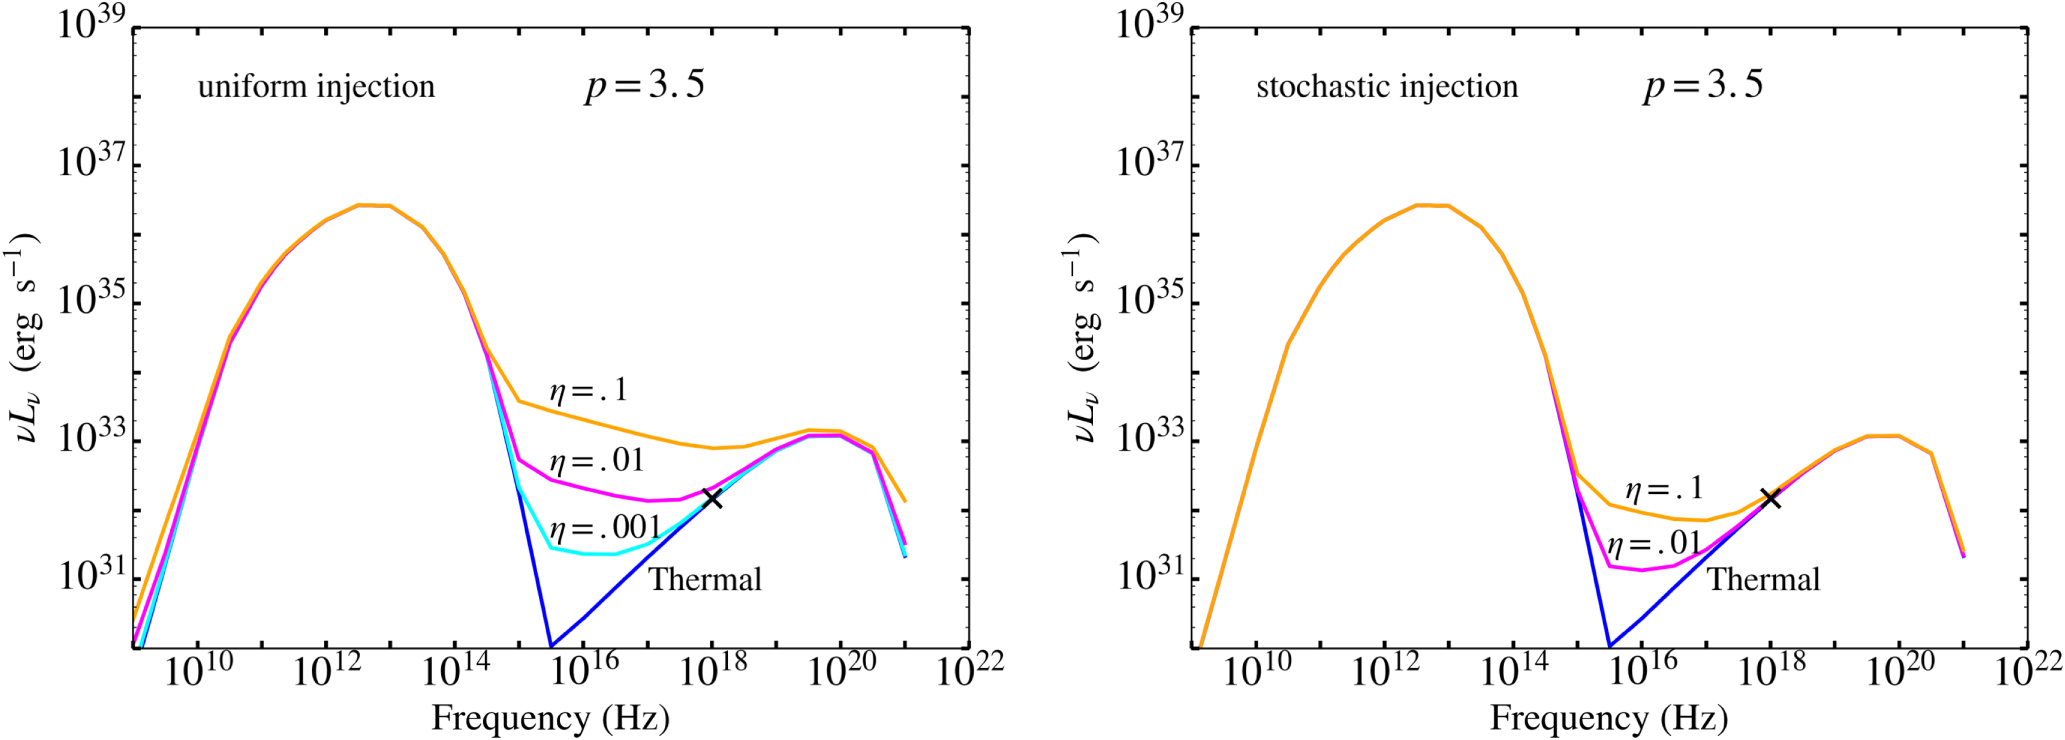
\includegraphics[angle=0,width=\columnwidth]{paper1_fig1}
\caption{Left: Spectra computed for quiescent (i.e., non-flaring) times for various values of the energy fraction of non-thermal electrons, $\eta$ with fixed power-law index, $p=3.5$, as well as for the purely thermal model.  In this configuration where the non-thermals only follow the thermal energy, the observed quiescent X-ray flux at $10^{18}$ Hz (depicted with an X) is exceeded even for moderate values of $\eta$.  Right: In this configuration, non-thermal electrons are injected in regions below $\beta=0.2$.  Localizing the non-thermal electrons to highly magnetized regions, where they are more likely to be accelerated, allows for significantly higher values of $eta$ while still accommodating the observed quiescent X-ray flux at $10^{18}$ Hz}
\label{fig1}
\end{figure}

In the right panel of Figure 1, we show the spectrum from the nonuniform stochastic model, where nonthermal electrons are localized to low-$\beta$ regions, again
with a power-law index of 3.5. Because of this localization, it is possible to accommodate higher fractions
of non-thermal electrons while still matching the quiescent thermal spectrum. In this model, it is possible
to inject almost 10\% of the total thermal energy into a
non-thermal electron distribution within the magnetized regions.
\section{X-Ray Variability: Stochastic Injection}


\begin{figure}
	\centering
	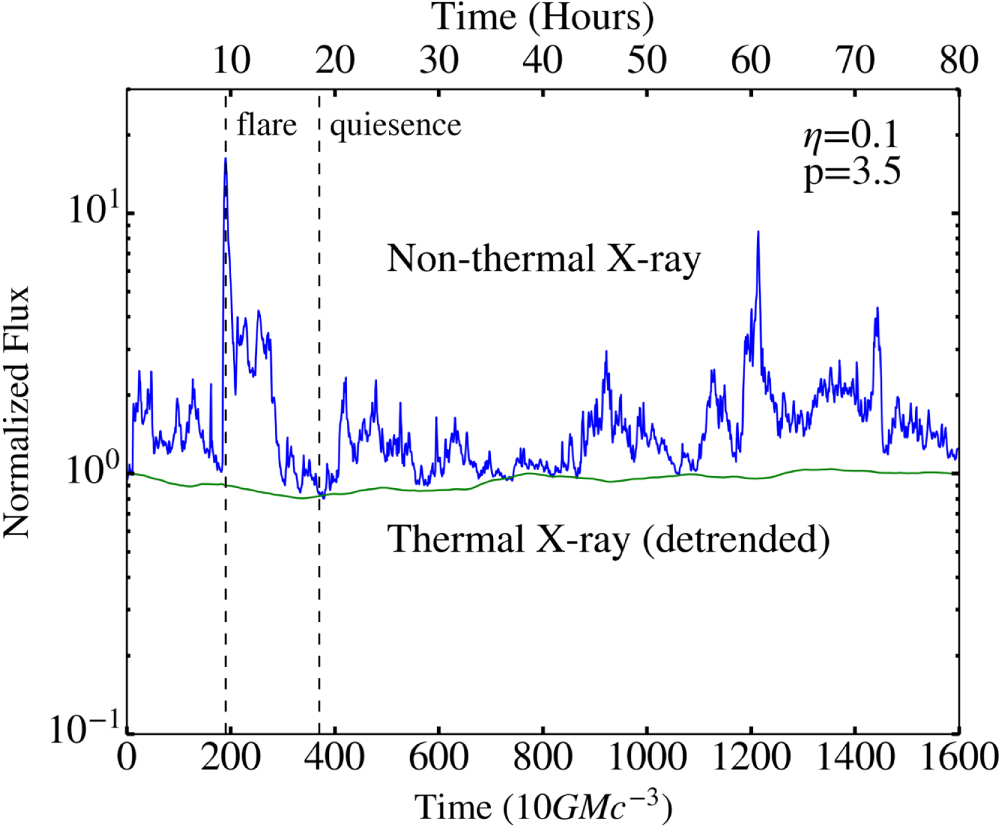
\includegraphics[angle=0,width=\columnwidth]{paper1_fig2}
	\caption{Thermal and non-thermal X-ray lightcurves.  The injection of non-thermal electrons into highly magnetized regions naturally produces significant variability due to the dynamic nature of magnetic fields in the accretion flow.}
	\label{fig2}
\end{figure}


\begin{figure}
	\centering
	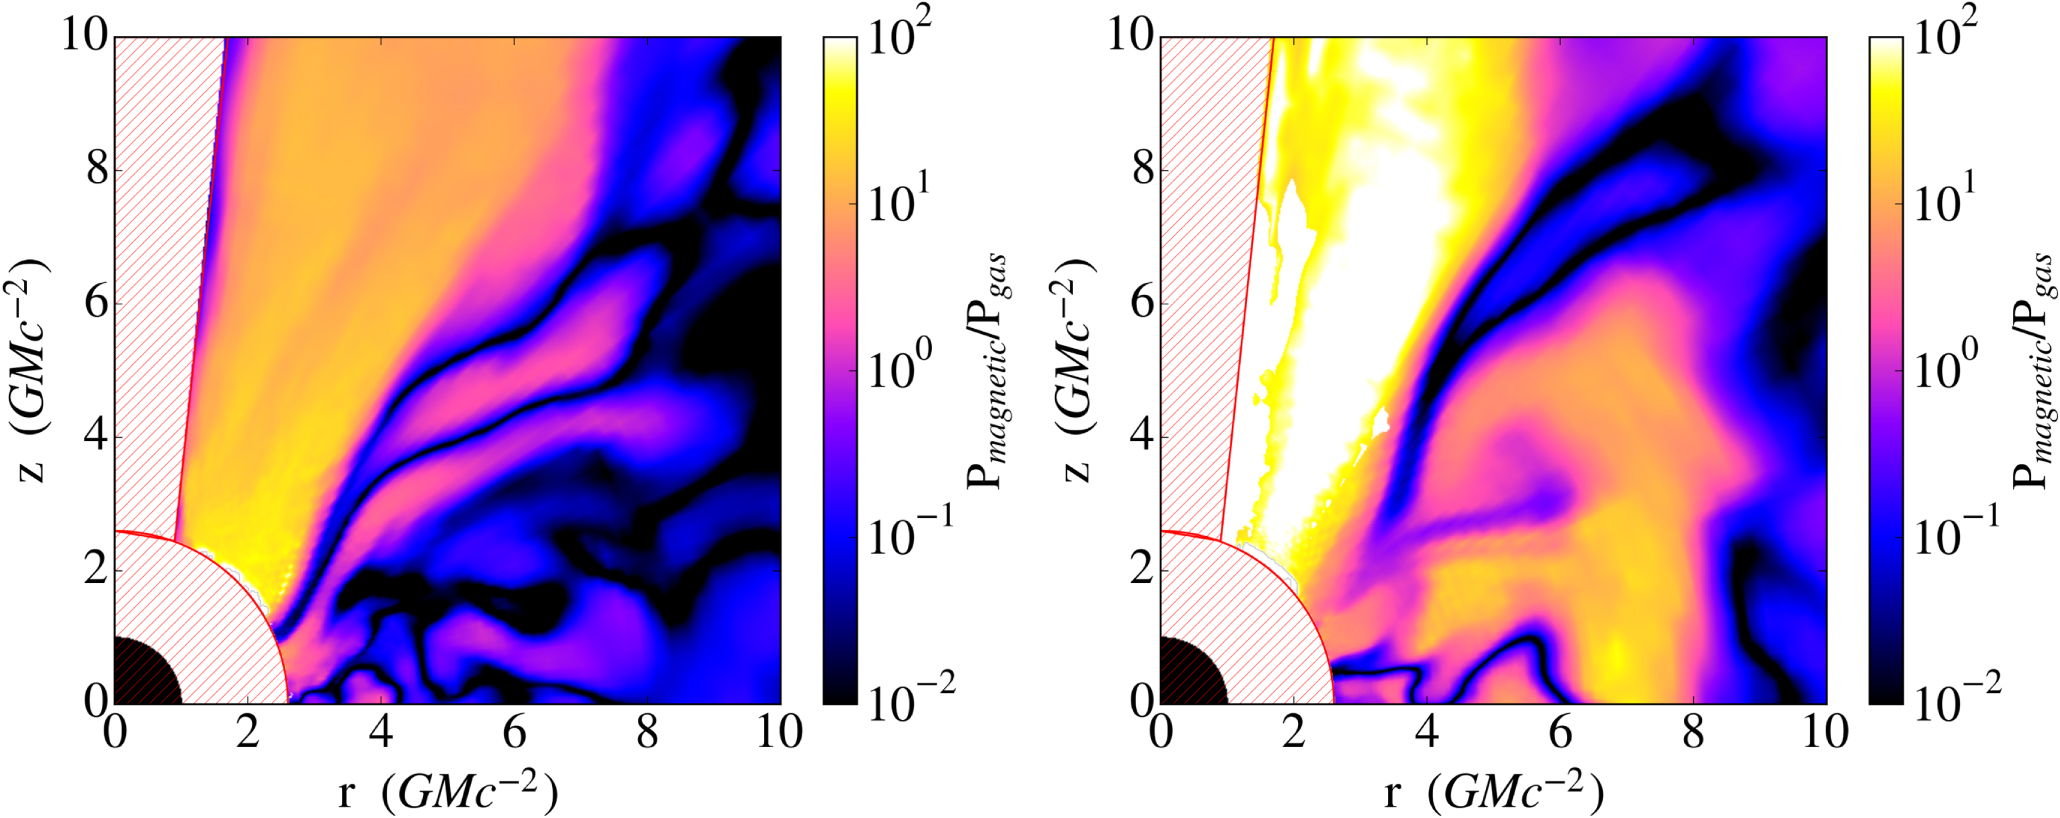
\includegraphics[angle=0,width=\columnwidth]{paper1_fig4}
	\caption{Left: Map of the ratio of the magnetic to gas pressure during a quiescent state in the simulation.  Cells near the pole and within the ISCO at $\sim 2.4 GMc^{-2}$ are excised due to numerical artifacts often occurring within these regions.  The black quarter-circle at the origin is the event horizon of the black hole.  Right: A large flux tube is present in the accretion flow during this flare, with high magnetization, resulting in a high ratio of pressures throughout a large portion of the disk. }
	\label{fig3}
\end{figure}

\begin{figure}
	\centering
	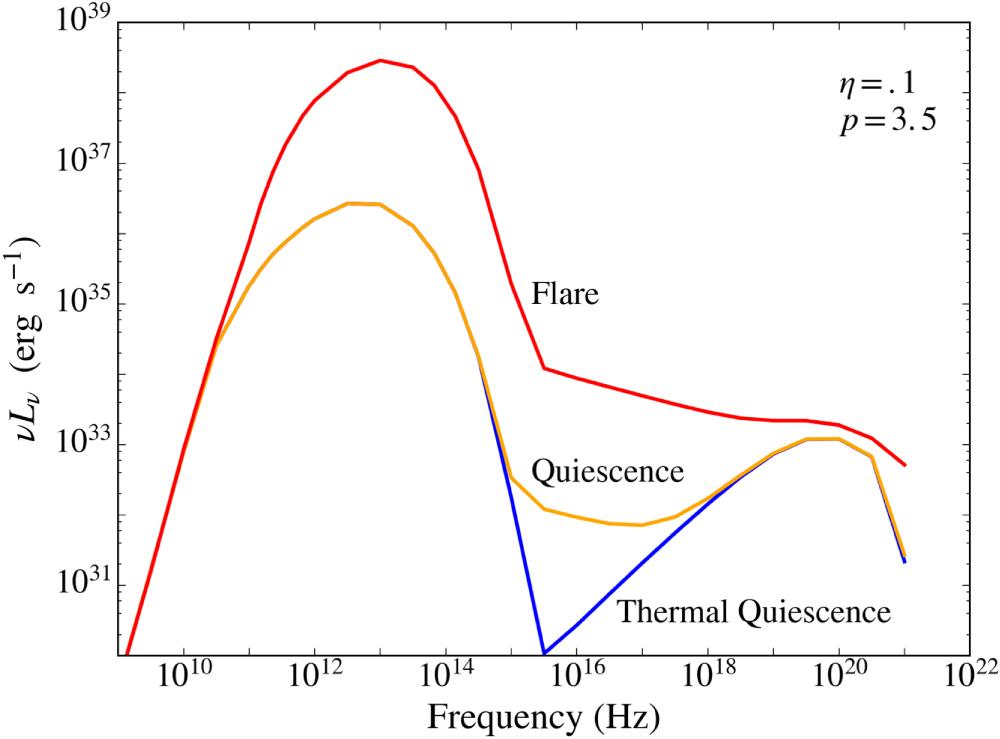
\includegraphics[angle=0,width=\columnwidth]{paper1_fig3}
	\caption{Spectra of the flaring and quiescent states depicted in Figure 3 in red and orange, respectively.  The purely thermal quiescent spectrum is shown for reference in blue. }
	\label{fig4}
\end{figure}

\begin{figure}
	\centering
	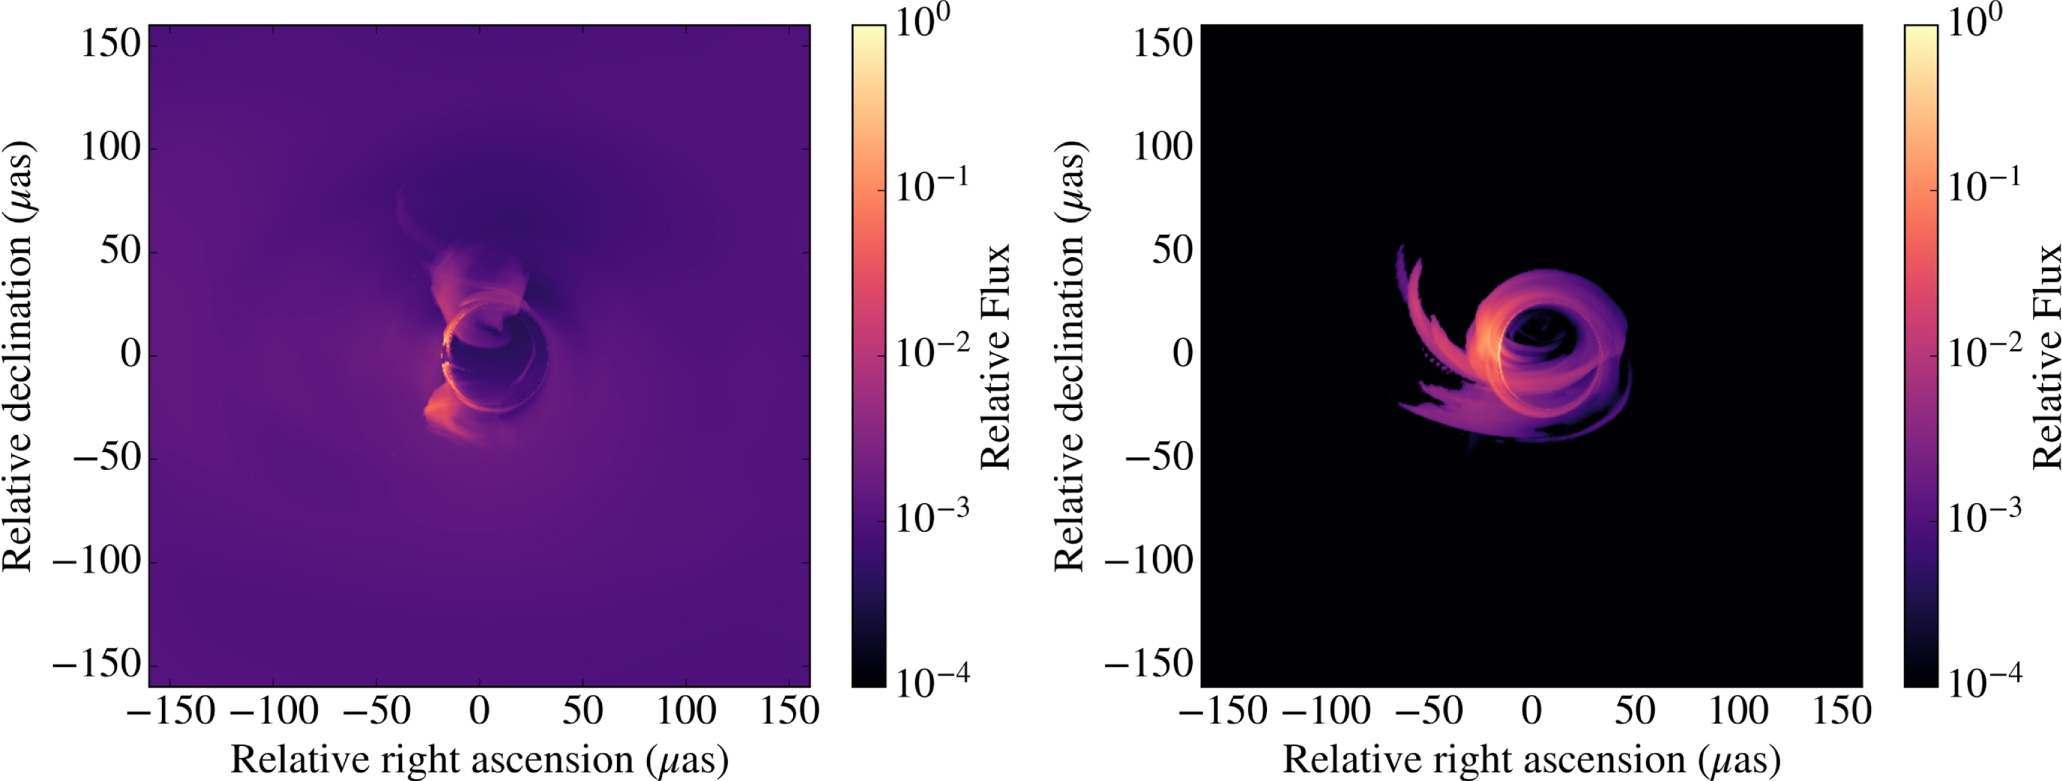
\includegraphics[angle=0,width=\columnwidth]{paper1_fig5}
	\caption{Left: Simulated image of quiescent X-ray (4.1 keV) emission. Fluxes are normalized to the maximum pixel value. Some
		structure is visible in the innermost regions of the image, where strong magnetic fields in the funnel close to the event horizon have
		associated non-thermal particles, and hence strong X-ray emission. We see that the extended Brehmsstrahlung emission comprises a
		significant fraction of the total flux during quiescence. Right: During the flare, emission is heavily dominated by the innermost part of the
		accretion flow; the relative contribution from the halo of Bremsstrahlung emission is negligible during flares.}
	\label{fig5}
\end{figure}

Apart from providing a more natural match to quiescent-state constraints, another interesting result
of using the $\beta$-dependent description of non-thermal electron injection is that it produces significant X-ray
variability. Perhaps this is not surprising, since the non-thermal electrons will trace magnetic flux tubes,
which are dynamic structures, constantly being formed, sheared, and moving throughout the flow. If one of these
flux tubes crosses a caustic behind the black hole, it will result in an additional amplification of the flux, and
since these tubes are emitting primarily non-thermal synchrotron radiation in the X-rays, they will cause X-ray
flares. We explore this variability in Figure \ref{fig2}, where we show the effect of stochastic injection of non-thermal electrons and compare it to a purely thermal model. In the nonthermal lightcurve, we see both persistent variability as
well as 4 large flares during the $\sim$80 hours of simulation. In the largest flares, the flux increases by a factor of $\sim 10$
compared to quiescence. The magnetically dominated regions responsible for these flares live for about 5000
seconds, which sets the timescale of the flares in this figure. There is indeed a stark contrast between this
result, which takes into account acceleration in low-$\beta$ regions, and the purely thermal model, which shows no variability.  We now investigate the properties of the magnetic structures in the innermost regions of the accretion flow
to further pinpoint the localization and time evolution of the flares. Figure \ref{fig3} shows the ratio of the magnetic
to the gas pressure throughout the inner flow during a
quiescent state and during the strongest flare from the
simulation. We see that this flare is caused by a large
magnetic flux region developing in the flow with $\beta < \beta_t$.
Due to the large spatial extent of this tube, many nonthermal electrons are injected, causing a sudden increase
in the X-ray flux. In contrast, during quiescence, the only
region with a significant number of non-thermal electrons
is in the funnel, which typically has a fairly uniform and
strong magnetic field. This only contributes a small flux
and results in low level variability.
Figure \ref{fig4} depicts the spectra of the flaring and quiescent
states from the simulation. During quiescence, the nonthermal emission is not especially prominent; its nature is
largely obscured by the thermal emission dominating at
most wavelengths. During the flare, however, the powerlaw nature of the non-thermal emission becomes more
evident.
In Figure 5, we show the X-ray images of our model
during flaring and quiescent states. The images show
the relative contribution to the overall flux from various
parts of the accretion flow. During quiescence, we find
that while there is some contribution to the X-ray flux

from a small population of non-thermal particles in the
funnel, the extended Bremsstrahlung emission accounts
for the majority of the total (i.e., integrated over the entire image) observed flux. During a flare, the emission is
heavily dominated by non-thermal electrons in the inner
accretion flow, rendering the Bremsstrahlung flux negligible. The difference in the localization of the X-rays
between the non-thermal and thermal models is responsible for their different variability properties.

\section{Comparison to Observations}
By interpreting observations of Sgr A* in the context of our GRMHD simulations, we begin to place constraints on the population of non-thermal electrons in the radiatively inefficient accretion flow and gain insight into their injection mechanisms. We employed two configurations for non-thermal electron injection, one in which the non-thermal electrons simply track the thermal energy everywhere throughout the flow and another where the non-thermal electrons are injected solely into regions of high magnetization. From the first model we are able to place tight constraints on the fraction of steady-state non-thermal electrons that may exist throughout the flow by comparing the simulations to the observed quiescent X-ray flux. The second model localizes non-thermal electrons to a much smaller region, allowing their local energy density to be much higher than the uniform model (by about 2 orders of magnitude) while still matching the
observed quiescent X-ray flux.


\begin{figure}
	\centering
	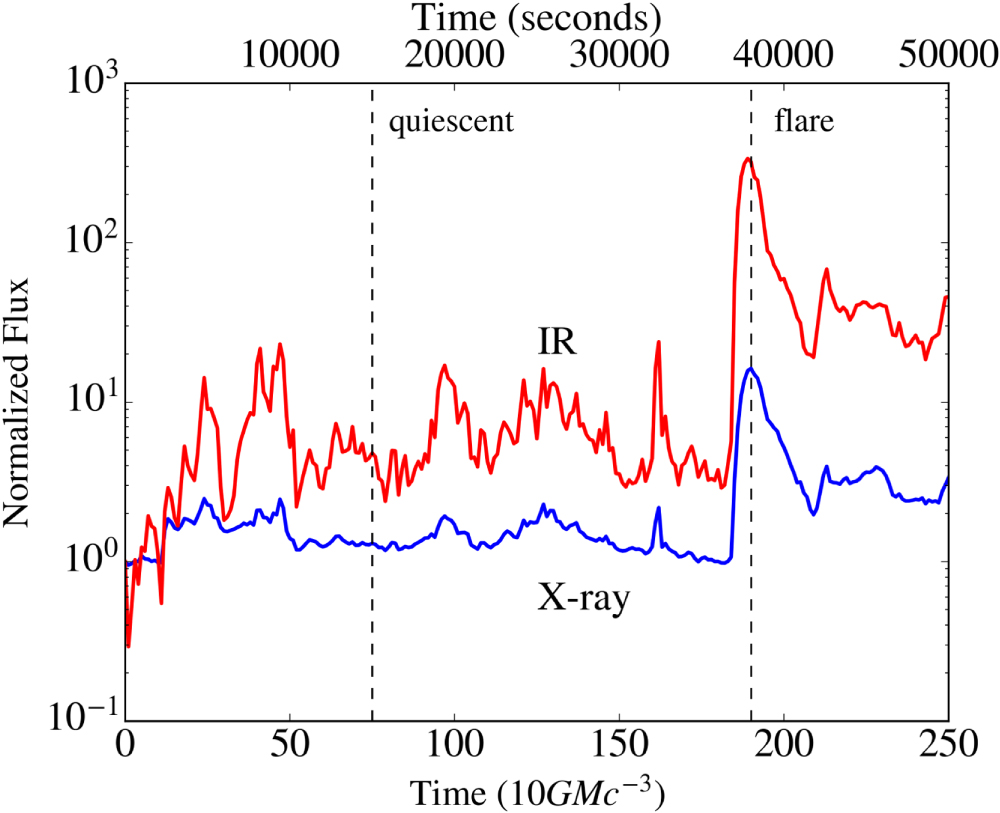
\includegraphics[angle=0,width=\columnwidth]{paper1_fig6}
	\caption{IR and X-ray lightcurves zoomed in on the first 250 timesteps of the simulation.  Each curve is normalized to a fiducial quiescent flux.  Note the strong and rapid variation in the IR flux and moderate variability in the X-ray.  The IR flaring has been described in \citet{chan2015b}.  The includsion of non-thermal electrons in highly magnetized regions has produced significant X-ray variability which was previously unseen.}
	\label{fig6}
\end{figure}

\begin{figure}
	\centering
	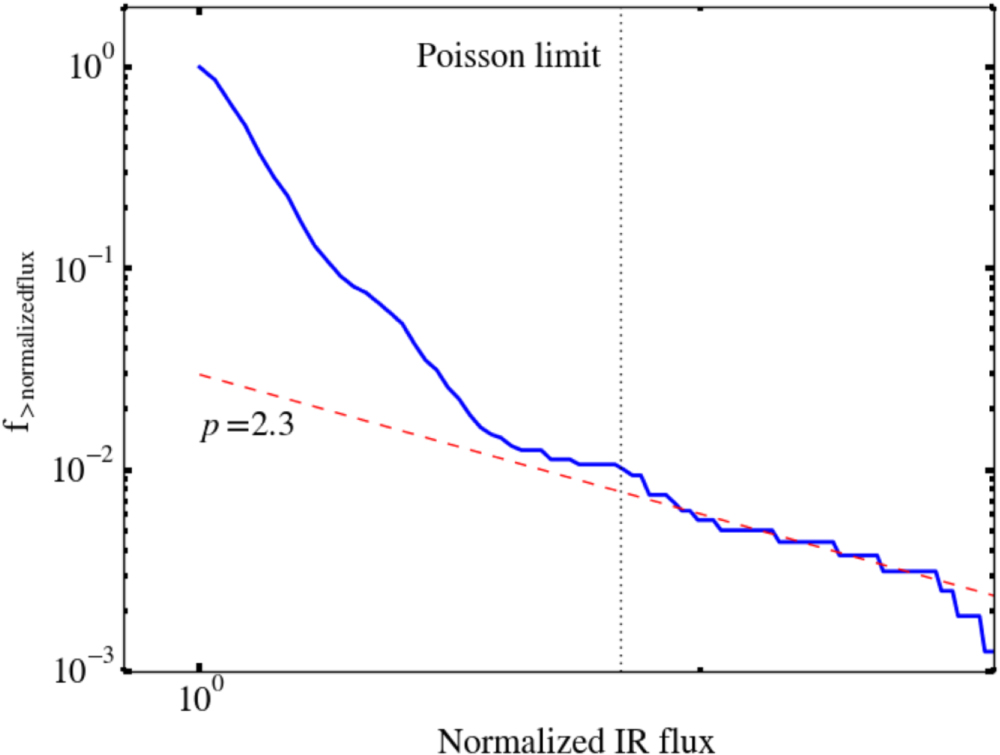
\includegraphics[angle=0,width=\columnwidth]{paper1_fig7}
	\caption{X-ray flux distribution, accounting for a constant quiescent background.  At high fluxes, the flare distribution resemble a power-law with an index of $\sim 2.3$.  Using the Poisson rate and binning reported in \citet{neilsen2015} for the Chandra observations used in that study, we estimate what would be the upper end of the Poisson-dominated regime, depicted with a vertical dotted line.}
	\label{fig7}
\end{figure}

\begin{figure}
	\centering
	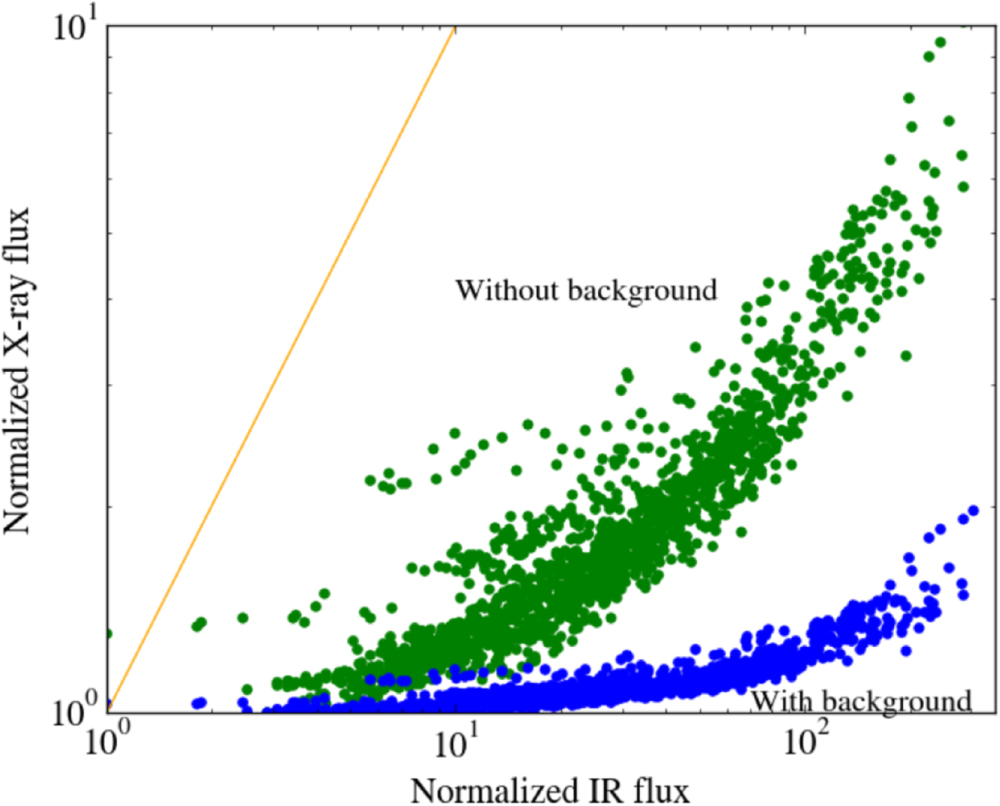
\includegraphics[angle=0,width=\columnwidth]{paper1_fig8}
	\caption{IR vs. X-ray flux, accounting for a constant quiescent background of X-ray flux (blue), and purely for the inner accretion flow (green).  The orange line depicts a correlation with a slope of unity.  The addition of the queiscent background decreases the X-ray variability by a factor of $\sim 10$.  We see a general trend of higher IR fluxes being associated with relatively high X-ray fluxes.}
	\label{fig8}
\end{figure}



We find that X-ray variability is a generic result of constraining the non-thermal electrons to highly magnetized regions. This is because the magnetic field is
dynamic throughout the flow, generating magnetic flux tubes, which are in a constant state of being formed, sheared, becoming buoyant, and leaving the disk. The
dynamic nature of these flux tubes combined with strong lensing effects from the black hole generate both persistent variability as well as flaring events.
X-ray flares in our simulations are always coincident with IR flares, but there are numerous IR flares without
X-ray counterparts, as shown in Figure \ref{fig6}, which qualitatively matches observations. In this figure, we have zoomed in to the first 250 timesteps of the simulation in order to more clearly illustrate the relationship between the IR and X-ray lightcurves. During this time span,
we observe about 5 IR flares over the stochastically variable background and one significant X-ray flare. From our simulation we find that there are about 5 IR flares per X-ray flare and a rate of one X-ray flare per 72,000 seconds, over the entire simulation. Over the course of
3 million seconds of observation with Chandra, 39 Xray flares were observed, corresponding to one flare every $\sim$77,000 seconds. Observations Sgr A* show that,
for every X-ray flare, there are about 4 NIR flares (e.g., \citealt{genzel2003, eckart2006}). These numbers
are in rough agreement with our results. In order to compare flare statistics from our simulations to observations more directly (e.g., through flux
distributions reported in Neilsen et al. 2015), we need to account for the fact that only  $\sim 10\%$ of the X-ray
emission from Sgr A* comes from the inner accretion flow (Neilsen et al. 2013). In Figure \ref{fig7}, after adding a
constant background equal to 90\% of the observed quiescent flux to our lightcurve from Figure 2, we plot the
flux distribution in our simulations. We find that the flare distribution resembles a power-law with an index of
around 2.3, while the lower-level variability does not have an obvious structure. Neilsen et al. (2015) reports only
Poisson variability at low fluxes, and power-law behavior at high fluxes, with a power-law index of 1.92. This is
roughly consistent with our simulated flux distribution. Our simulations, however, do not account for the Poisson photon counting noise, and also do not show as large of a range of variability. The latter is likely due to the
relatively short duration of our simulation that did not capture many rare, high flux events.
We estimate the level of the Poisson noise, below which we expect our simulated flux distribution to deviate significantly from observations. We take the reported photon counting rate ($Q = 5.24$ cts/ks) and binning ($b = 300$ s) from Neilsen et al. (2015) and calculate the typical fractional Poisson error, $\epsilon=1/\sqrt{Qb}=0.79$. Normalizing our lowest level of emission to 1, we see that counting noise
will dominate the observed variability from 1 to $1+\epsilon$,
setting the lower limit from which we expect our simulations to reproduce the flux distribution.
We further explore the relationship between IR and Xray fluxes in Figure \ref{fig8}. The largest IR flares correspond
to the largest X-ray flares, but there is much more variability in the IR than the X-rays. In our simulations,
anytime a flux tube appears and crosses a caustic there
will be an IR flare due to the synchrotron emission from
the thermal electrons. However, only the most highly
magnetized flux tubes will have non-thermal electrons
associated with them and will generate an X-ray flare.
The effect of the $\beta$ threshold is to pick out a subset of all
the magnetic flux tubes, ones with conditions suitable for
reconnection to occur. The particular threshold we use is
motivated by \citet{liguo2015}, who showed a non-thermal
component being generated for $\beta < 0.2$. As a result, IR
variability is much more significant, since there is thermal synchrotron associated with all flux tubes, whereas
particle acceleration and hence X-ray emission only occurs for a particular subset of the tubes. Additionally,
we see that the flux tubes responsible for the largest IR
flares are the same structures responsible for the largest
X-ray flares. This is unsurprising given the strong scaling
of synchrotron emissivity with magnetic field; the most
highly magnetized flux tubes radiate copiously in the IR
due to the high magnetic fields, and also act as sites of
efficient reconnection, generating strong X-ray flares.
\section{Conclusions}
In this paper, we explored the effects of incorporating non-thermal electrons into GRMHD simulations of
radiatively inefficient accretion flows. We found that
X-ray variability is a generic result of constraining the
non-thermal electrons to highly magnetized regions and
that the timescales associated with electron cooling are
comparable to the observed flare duration. This analysis is model-dependent, since the synchrotron radiation
from non-thermal electrons depends on the strength and
topology of the magnetic field, which will impact the constraints we place on the quiescent energy budget of the
non-thermal electrons. Our analysis of cooling timescales
are also likely to differ across models. For model B with
only inflowing velocities within 10 gravitational radii, we
found that flares are unlikely to originate from the funnel since the inward radial velocities were too large to
explain the X-ray flares lasting many thousands of seconds. We will explore the role of non-thermal electrons
in producing the variability for different magnetic field
configurations and black hole spins in a future study.
In the context of model B, which has matched many
observational constraints, from the quiescent broadband
spectrum to the variability properties, we find that Xray flares likely originate from magnetic flux tubes in the
disk, where centrifugal support allows the non-thermal
electrons to remain in the flow for many thousands of seconds while radiating away their energy via synchrotron
emission. The flare lengths are hence set by the synchrotron cooling timescales. The properties of the Xray variability from this model are consistent with observations: X-ray flares are always coincident with IR
flares, there are many more IR flares without associated
X-ray counterparts, and the timescales associated with
the flares are comparable to the observed flare duration.
\chapter[The Properties of Reconnection Current Sheets in GRMHD Simulations of Radiatively Inefficient Accretion Flows]
{The Properties of Reconnection Current Sheets in GRMHD Simulations of Radiatively Inefficient Accretion Flows}

\section{Introduction}
In this chapter, we use representative GRMHD simulations to assess whether reconnection regions frequently
occur in global simulations. We consider simulations
with Standard and Normal Evolution (SANE) and Magnetically Arrested Disk (MAD) initial magnetic field configurations (e.g., \citealt{narayan2012}). In the SANE case, the magnetic field is initialized with alternating poloidal loops, while the MAD initial field consists of a single poloidal loop, which results
in the magnetic field playing a more dominant role in
the dynamics of the disk. We devise criteria to locate
regions of field reversal and characterize the properties
of the plasma in these regions. We focus on the plasma-$\beta$
and magnetization parameter $\sigma$, which have been shown
to play an important role in particle acceleration. We
also identify field components that are orthogonal to
the reversing field, often referred to as guide fields, and
quantify their strengths. Our results will guide future
particle-in-cell (PIC) studies of low-luminosity accretion
flows. Finally, we compute the time-dependent magnetic
energy available in reconnection regions to assess whether
this is a plausible mechanism to generate the observed Xray variability of Sgr A*.

\section{Characterizing Potential Reconnection Regions in MHD Simulations}
Magnetic reconnection takes place in regions where
there is a reversal of magnetic field over a short characteristic length scale, in which the current density becomes large. In typical simulations of the local dynamics
of reconnection, the initial condition is specified in terms
of a Harris sheet, which has the magnetic field profile

\begin{equation}
	\bold{B} = B_0 \tanh{\frac{x}{L}}\hat{y}
\end{equation}

In this geometry, the y-component of the magnetic field
reverses direction over a characteristic length L in the
x-direction. This field reversal has a high curl associated
with it, leading to a sudden peak in the current density,
which scales as
\begin{equation}
	\bold{J}= \frac{B_0}{L}\rm{sech}^2\frac{x}{L}\hat{z}.
\end{equation}

There are only a small number of parameters that determine the particle heating and acceleration that results from reconnection events.  These are the magnetization parameter

\begin{equation}
	\sigma \equiv \frac{B^2}{4 \pi \rho c^2}
\end{equation}

which is the ratio of magnetic energy density to rest mass energy density, and the plasma-$\beta$ parameter

\begin{equation}
	\beta \equiv \frac{P_{\rm{gas}}}{P_{\rm{magnetic}}}=\frac{8\pi n k T}{B^2},
\end{equation} 

which specifies the ratio of gas pressure to magnetic pressure.  Here, $\rho$, $n$, and $T$ are the mass density, number density, and temperature of the plasma particles, respectively.

Another important quantity to consider for magnetic
reconnection is the magnitude and direction, if present,
of the so-called guide field. This is the component of the
magnetic field in the sheet perpendicular to the reconnecting field. The effect of such a guide field on particle
acceleration has been studied in certain regimes (\citealt{wang2016, dahlin2016, stanier2016}) and, in
some cases, can have an effect on the resulting electron
energy distribution.
Our first goal is to devise an algorithm that will allow
us to identify the location and relevant properties of potential reconnection regions, i.e., Harris sheets, in global
GRMHD simulations, which we describe in the following


\section{Finding and characterizing current sheets}
As an illustrative example, we use two 60 hr (about
$11,000 \; GM/c^3$
) long GRMHD simulations of a radiatively inefficient accretion flow onto a black hole
(\citealt{narayan2012}) that were
performed using the HARM code (\citealt{gammie2003}).
These simulations were employed in a large study of the
broadband, time-dependent emission from Sgr A* (\citealt{chan2015a,chan2015b}) where we coupled HARM to the radiative
transfer algorithm GRay (\citealt{chan2013}) and varied
the black hole spin, density normalization, observer inclination, initial magnetic field configuration, as well as
the electron thermodynamic prescription. From these
investigations, we identified 5 models that best fit the
steady-state broadband spectrum as well as the previously observed 1.3 mm image size of Sgr A* and also
characterized their variability properties. In the present
study, we use two representative models from \citet{chan2015b}: a SANE model with a black hole spin a = 0.7
and a MAD model with a black hole spin a = 0.9. In general, the thermal SANE models tend to show short-lived,
high amplitude variability in their IR and mm flux, while
the thermal MAD models tend to show lightcurves dominated by smooth and long-timescale flux changes.
Our goal is to identify in each snapshot from these simulations potential regions of reconnection. Because of the
large shear in the accretion flow, the magnetic fields are
primarily toroidal and the alternating components occur
primarily in the azimuthal direction. For this reason,
we search through the simulation volume for cells that
have both a high current relative to the mean value in
the snapshot as well as very low values of the azimuthal
component of the magnetic field $B_{\phi}$ in order to pick out
the sheets where reconnection may occur.
Specifically, we consider 2D slices of the simulation volume at each azimuthal angle $\phi$ at each snapshot and identify the points that (i) have current magnitudes $\sqrt{J_\mu J^\mu}$
that are higher than four times the mean current of that
snapshot and (ii) $\phi$-components of the magnetic field
smaller than a fiducial value, characterized by the usual
magnetization parameter $\sigma_\phi = B^2_{\phi}/(4 \pi m n c^2)$. We use a
$\sigma_\phi$ threshold of $10^{-6}$. We then apply an algorithm similar to the one described in \citet{zhdankin2013} for
identifying and analyzing the statistics of current sheets
in shearing box simulations of MHD turbulence. For every point with grid indices ($i$, $j$) on an azimuthal slice of
our domain picked out by the above criteria with current
magnitude $J_{\rm{peak}}$, we consider all 4 adjacent points in the
grid. If the current at an adjacent point is above $J_{\rm{peak}}/2$,
while also satisfying $\sigma_{\phi}<10^{-6}$
, we consider it as part
of the same current sheet. We continue this process of
scanning every point in the sheet, considering all neighboring points, and applying these criteria to them until
no more points are being added to the sheet.
In the top panel of Figure \ref{bphi_sheet_example}, we show the result of
applying this algorithm on a snapshot of the SANE simulation, with the $B_{\phi}$ configuration shown in the bottom
panel of the same figure. It is evident that the regions
between flux tubes of opposing azimuthal magnetic flux
are effectively picked out. When we repeat this procedure on all adjacent azimuthal slices, we find that the
current sheets show large azimuthal extents throughout
the flow, providing ample surface area for neighboring
flux tubes to reconnect over.  We show in Figure \ref{MAD_snapshot}, a representative
snapshot of the MAD simulation for comparison. We see that
the magnetic field strengths about the current sheet in the MAD
simulation are higher than that in SANE. Additionally, we find
that there is typically less fine structure to the MAD current
sheets; the MAD current sheets tend to consist of one or two
relatively flat sheets, while the SANE current sheets are often
highly curved and twisted into complicated geometries, as
shown in the top panel of Figure \ref{SANE_snapshot}.

\begin{figure}[!h]
\centering
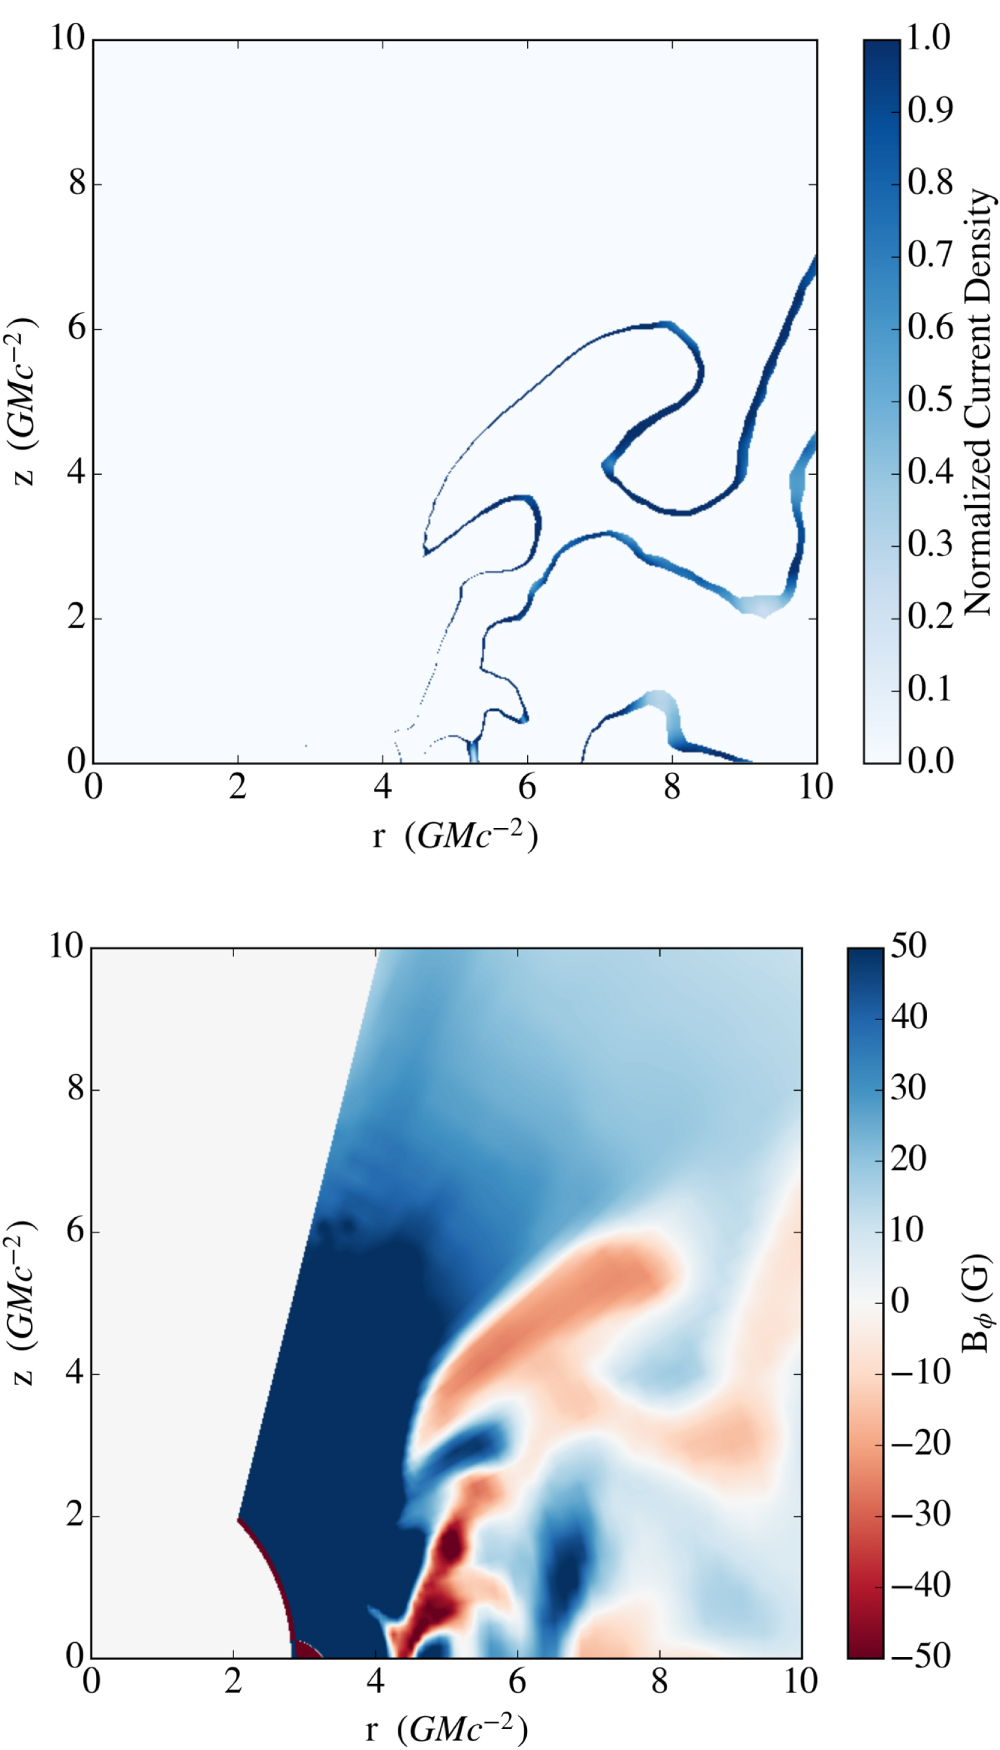
\includegraphics[width =.6\textwidth]{paper2_fig1.jpg}
\caption{(Top) The current sheets picked out by our algorithm in a SANE simulation, at the interface between regions of opposing magnetic flux.  Regions near the pole and within the ISCO are excised to avoid known numerical issues related to the density floor imposed.  (Bottom) A 2D slice of the azimuthal magnetic field in one snapshot of the SANE simulation, showing the presence of numerous opposing flux tubes that provide potential sites of reconnection.}
\label{SANE_snapshot}
\end{figure}


\begin{figure}[!h]
	\centering
	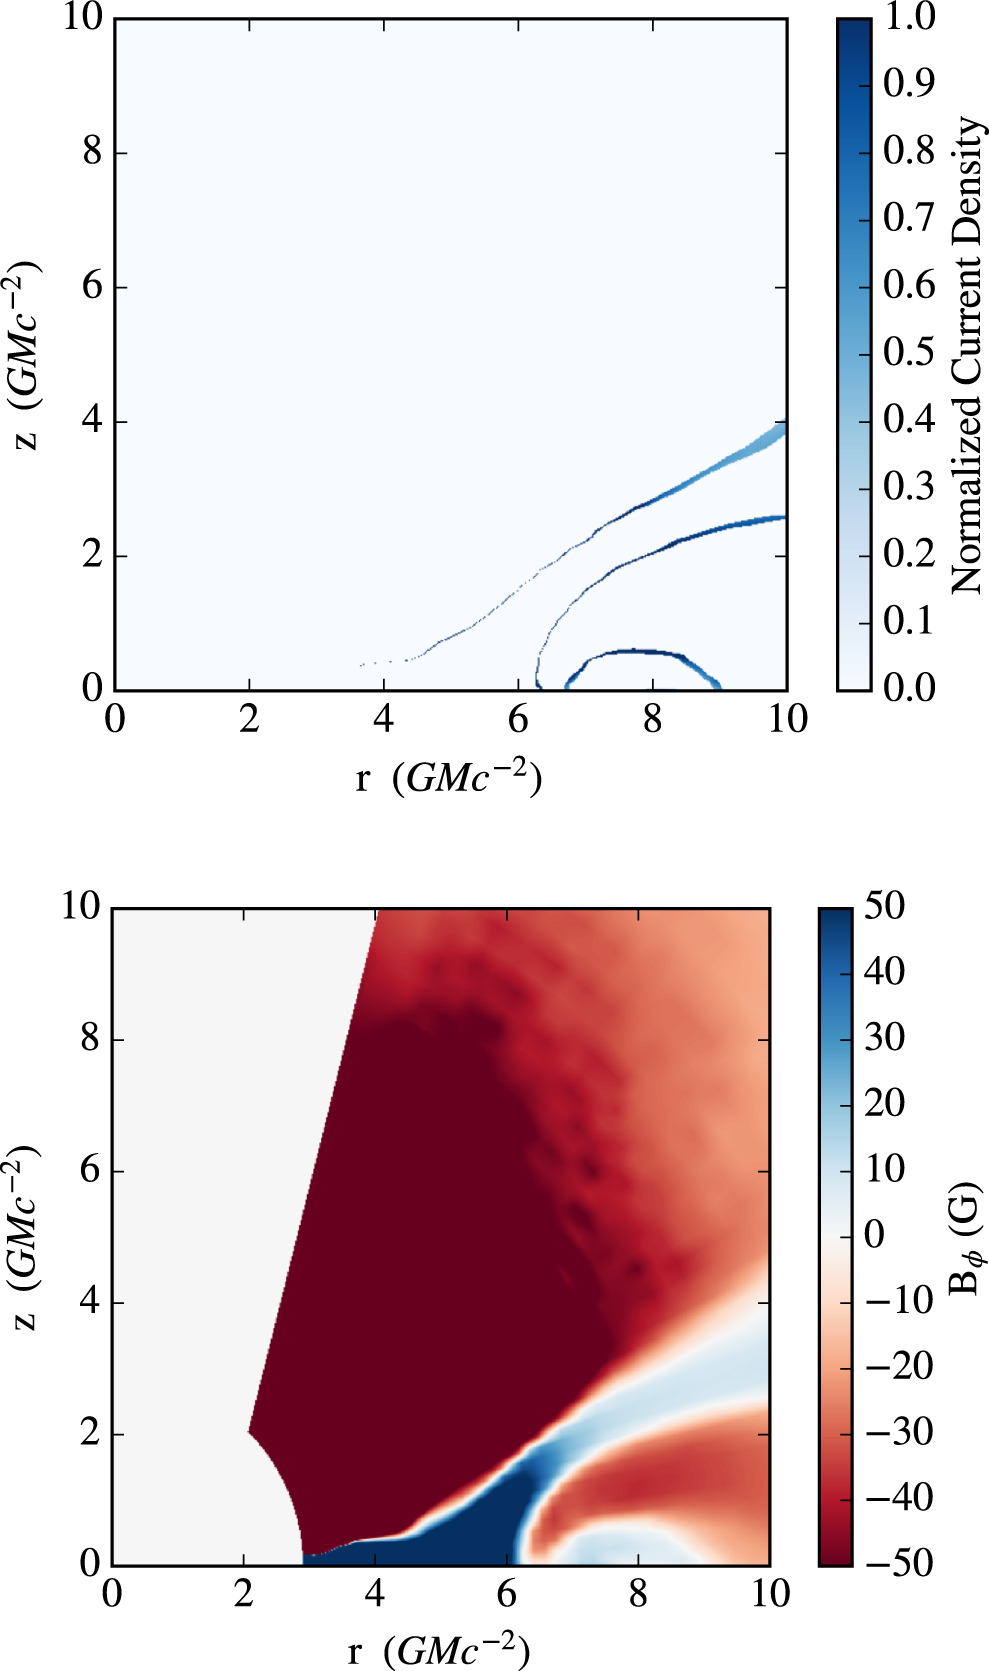
\includegraphics[width =.6\textwidth]{paper2_fig2.jpg}
	\caption{Top: the current sheets picked in a MAD simulation.  Bottom: a 2D slice of the azimuthal magnetic field in one representative snapshot of the MAD simulation.  We see that the typical toroidal field strengths are higher, and that there is generally less structure as compared with the SANE simulation.  We see these difference between SANE and MAD in the majority of snapshots from our simulations.}
	\label{MAD_snapshot}
\end{figure}

\subsection{Sampling Plasma Properties Associated with Current Sheets}
Once we identify the current sheets in each snapshot,
we characterize the plasma parameters of these sheets
that are relevant to magnetic reconnection. The location
that we want to measure these parameters at is not in
the sheet itself but where the magnetic field reaches its
asymptotic value some distance away from the sheet in
a direction perpendicular to it. This breaks down into
two problems: finding the direction perpendicular to the
sheet and determining how far to go along this direction
until the magnetic field reaches its appropriate asymptotic value. 

In order to approximate the direction perpendicular to
the current sheet at a point ($i$, $j$) that has been flagged
as belonging to the sheet, we first find the local slope of
the sheet about this point. To do this, we consider a box
around each point ($i$, $j$) in the sheet, with width $S+1$,
whose corners are at ($i \pm S/2$, $j \pm S/2$). We use a value
of $S = 10$ pixels, which is generally smaller than the
radius of curvature of a current sheet. We then calculate
the slope from the point in the center of this box ($i$, $j$)
to every other point ($i'$, $j'$)
in the box which is flagged
as being part of the current sheet. Taking the inverse
tangent of this slope gives the angle with respect to the
horizontal of the line that passes through ($i$, $j$) and ($i'$,$j'$.
We calculate the average of these angles, approximating
the angle of the current sheet about point ($i$, $j$) as
\begin{equation}
\theta_{mean}=\frac{1}{N}\sum_{\left(i',j'\right)_{1}}^{\left(i',j'\right)_{N}}\arctan{\left[\frac{z(j'_n)-z(j)}{r(i'_{n})-r(i)}\right]}
\end{equation}

We then calculate the mean slope:
\begin{equation}
m_{mean}=\tan{\theta_{mean}}
\end{equation}

and take the direction perpendicular to this slope:

\begin{equation}
m_{\perp}=-\frac{1}{m_{mean}}
\label{meanslope}
\end{equation}

We sample the plasma properties at some distance
along the normal where the toroidal magnetic field has
reached its asymptotic value. We approximate this location by scanning along the normal direction, given by
Equation \ref{meanslope}, until the field profile flattens out. We consider the field sufficiently flat when the fractional change
in magnetic field from one computational cell along the
normal to the next is less than three percent, averaged over two adjacent cells\footnote{Even though the approach outlined here for the definition of orthogonal directions is valid only for a flat spacetime, it is adequate for our present purposes both because we deal with short distances ($\sim 0.1 M$) away from the current sheets and because we are interested in quantifying the typical values of the asymptotic magnetic field without being very sensitive to the precise direction.}

As an illustrative example, Figure \ref{fieldprof} shows the magnetic field
and current density profile along the normal of a current sheet
picked out by our algorithm in the SANE simulation (the
typical shapes of these profiles generalize to the MAD
simulations). We indeed see a Harris-sheet-like structure, with
a magnetic field profile that passes through 0 and asymptotes to
a fixed value at a distance $\approx 0.2-0.3 GMc^{-2}$ away from the
center; the current density has the expected maximum
associated with the steep gradient in magnetic field. To
illustrate the variety of current sheets and show their typical
length scales and field profiles, Figure 4 shows a sample of
current sheets identified in different snapshots and locations of
the SANE simulation. The magnetic field profiles again follow
structures reminiscent of Harris sheets, with the magnetic field
passing in a linear fashion through 0 and reaching an
asymptotic value at a distance that is typically $0.2$ to
$0.6 GMc^{-2}$ away from the center of the sheet. We find that
while the current sheets are often approximately symmetric
(approaching similar magnetic field strengths to either side of
the current sheet), there are also cases of non-symmetric current
sheets, where the asymptotic magnetic field strength differs
between the two sides of the sheet. Studies of magnetic
reconnection almost always employ symmetric current sheets,
but the asymmetry in magnetic field profile could influence the
outcome of reconnection.


\begin{figure}[!h]
	\centering
	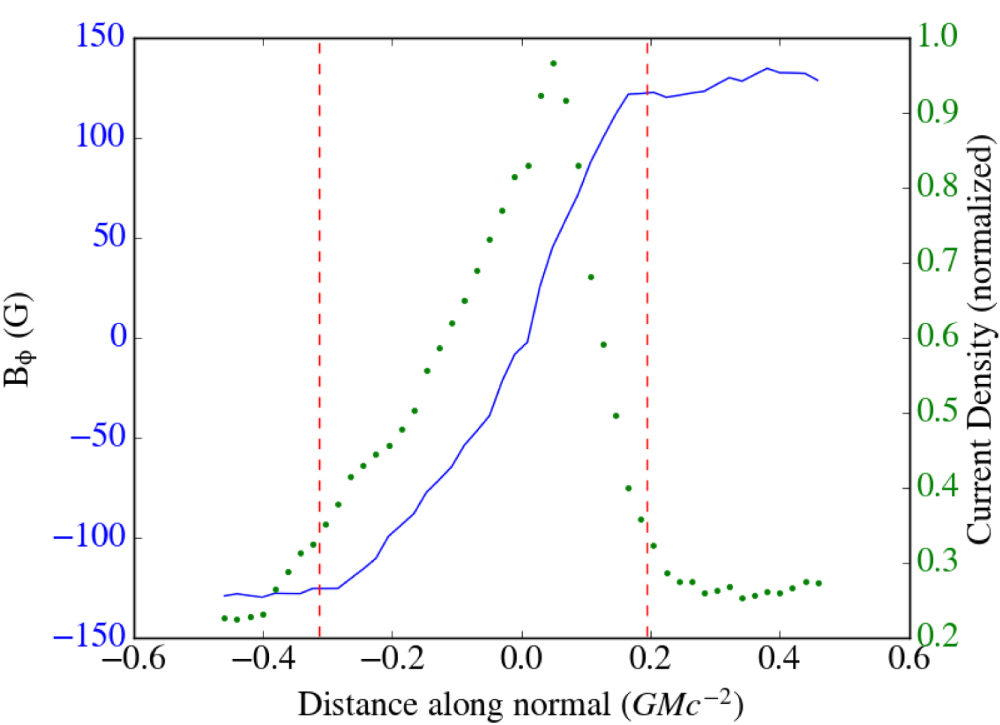
\includegraphics[width =\textwidth]{paper2_fig3.jpg}
	\caption{Magnetic field (blue line) and current density (green points) profiles
		along the normal direction to a current sheet showing the typical field reversal
		across the current sheet and the associated maximum in current density. The
		red dashed lines indicate the location at which we sample the relevant plasma
		parameters.}
	\label{fieldprof}
\end{figure}


\begin{figure}[!h]
	\centering
	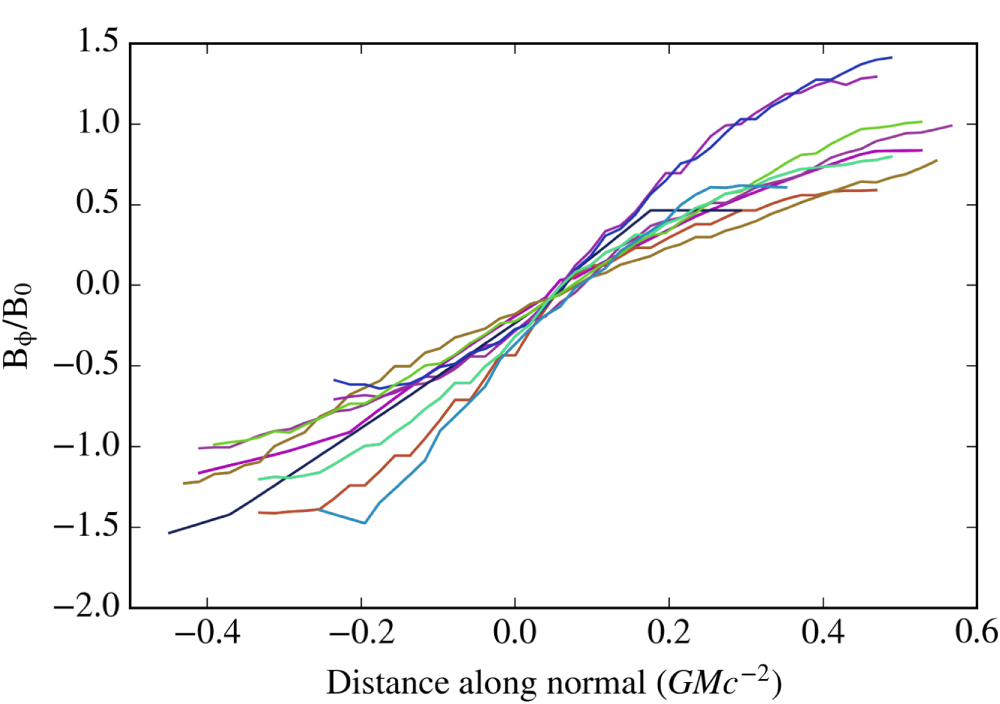
\includegraphics[width =\textwidth]{paper2_fig4.jpg}
	\caption{Random selection of field profiles from the simulation across current
		sheets, showing that the typical behavior is reminiscent of the idealized Harrissheet structure, passing linearly through 0 and asymptoting to similar values on
		either side of the sheet. The vertical scale is normalized to the average
		asymptotic magnetic field for each sheet.}
	\label{many_fieldprof}
\end{figure}

\section{Plasma Properties of Current Sheets}
Having established the frequent occurrence and geometry of potential reconnection regions, our second goal
is to investigate the properties of current sheets in timedependent simulations of accretion flows and characterize
the parameters relevant to non-thermal particle acceleration to inform further PIC studies. We ultimately wish to
determine the role of magnetic reconnection in contributing to the multiwavelength variability of low-luminosity
accretion flows.
Iterating through timesteps in our simulations, we
find the current sheets and, at every point in each sheet,
determine the asymptotic values of $\sigma$ and $\beta$ as well as
the guide field strength at the center of the sheet for
both our SANE and MAD simulations, as described
below.

\subsection{Properties of SANE Current Sheets}
For the SANE simulation, in the regions where reconnection may occur, the magnetization $\sigma$ ranges from $10^{-4}$ to 1, while the plasma-$\beta$ ranges from $0.1$ to $10^3$, as shown in Figure \ref{SANE_hist}
The anticorrelation evident in Figure \ref{SANE_hist} (see also Figure \ref{MAD_hist}) occurs because the magnetization parameter scales as $B^2/n$, while the plasma-$\beta$ scales as $(B^2/n)^{-1}$.  The spread arises because the plasma-$\beta$ also depends on the plasma temperature.



\begin{figure}[!h]
	\centering
	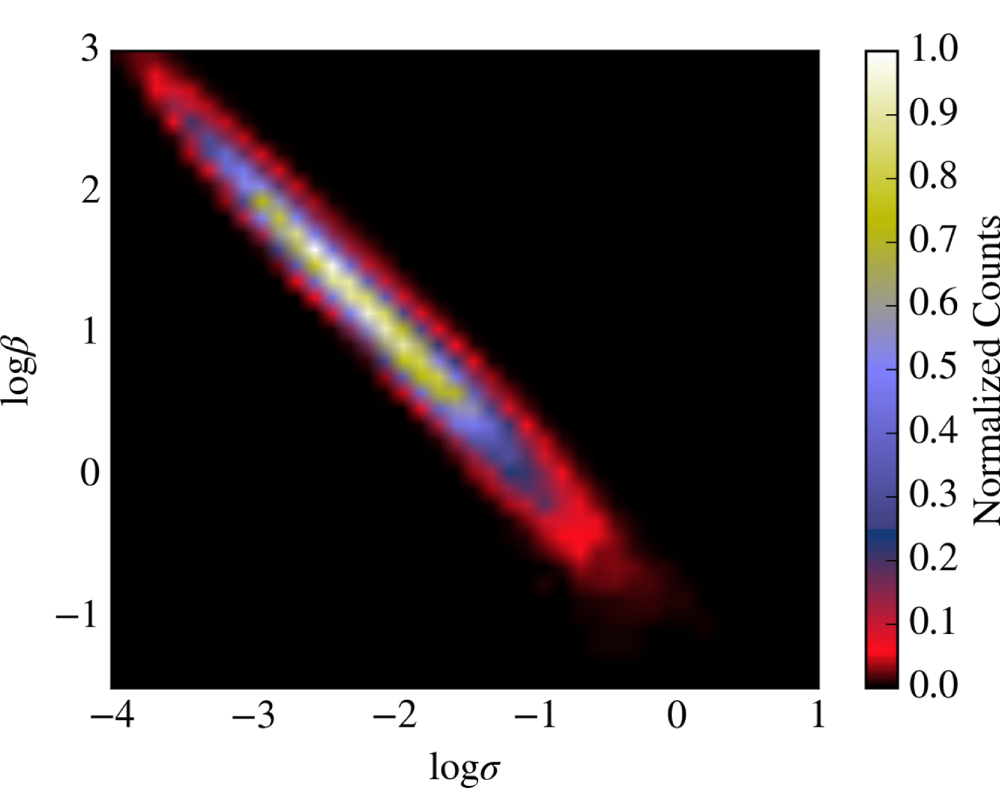
\includegraphics[width =\textwidth]{paper2_fig5.jpg}
	\caption{Two-dimensional histogram of the magnetization $\sigma$ and plasma-$\beta$ across all current sheets in the inner $10 \; GM/c^2$ of the SANE simulation.}
	\label{SANE_hist}
\end{figure}

\begin{figure}[!h]
	\centering
	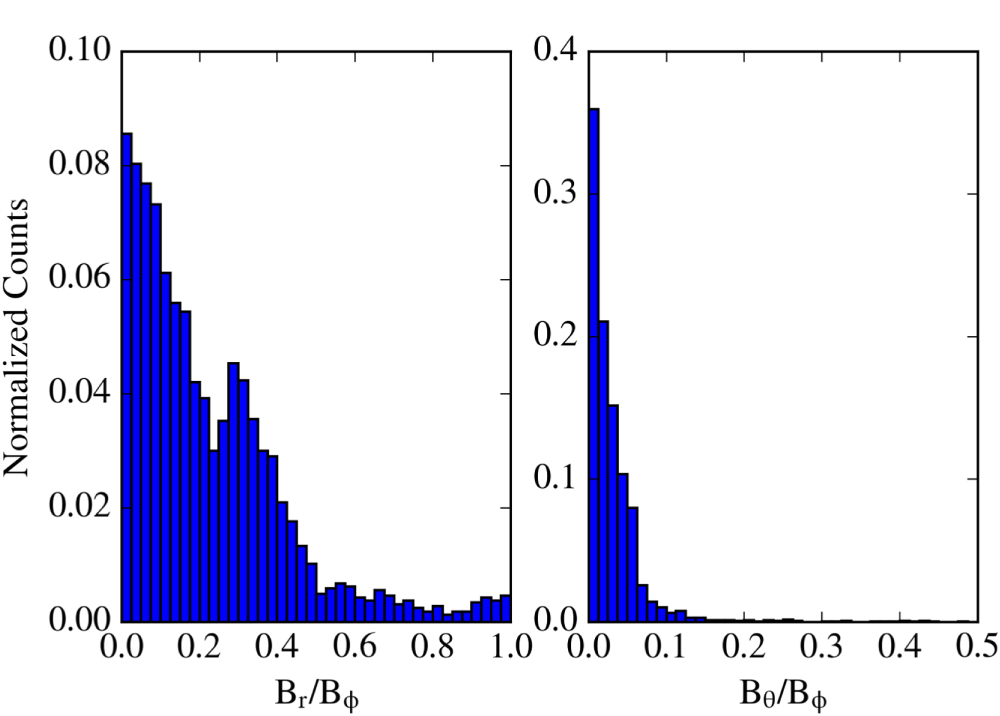
\includegraphics[width =\textwidth]{paper2_fig6.jpg}
	\caption{Histogram of guide fields in the SANE simulation, scaled to $B_{\phi}$, the component showing field reversal.  A large number of current sheets have no guide fields associated with them and, when present, the guide fields tend to be quite weak.}
	\label{SANE_bguide}
\end{figure}



The most promising subspace of this region for particle
acceleration to be efficient is the high-$\sigma$, low-$\beta$ (bottomright) regime, where there is maximal magnetic energy to
dissipate into the particles and fairly little gas pressure
relative to the magnetic pressure, such that the plasma is
magnetically dominated. The inferred ranges of $\sigma$ and $\beta$
are interesting for a number of reasons. Studies have only
recently begun for this transrelativistic regime (\citealt{werner2016})) and the physics of particle acceleration and
heating in these conditions are not yet fully understood.
While the ions in this regime remain non-relativistic (because $\sigma$ is of order 1), the electrons will likely be accelerated (or heated on average) to highly relativistic speeds,
since $\sigma_e \equiv B^2/(4\pi \rho_e c^2)=\sigma m_i/m_e \approx 10^3$, which is an
estimate of the characteristic electron Lorentz factors expected from reconnection.
Finally, in Figure \ref{SANE_bguide} we show a histogram of the relative guide field strengths in the SANE simulation. It is
evident that both cases of weak ($B_r/B_{\phi}] < 0.5$) and of no
guide fields are of interest for the purposes of these simulations. Even weak guide fields may play an important
and potentially adverse role in determining the outcome
of magnetic reconnection and must be explored via PIC simulations in the transrelativistic regime.

\subsection{Properties of MAD Current Sheets}

For the MAD simulation, we find that, in the regions of potential reconnection, $\sigma$ ranges from $10^{-3}$ to $10$, while $\beta$ ranges from $0.03$ to $10^{3}$ , as shown in Figure \ref{MAD_hist}. This is roughly an order of magnitude higher (lower) than the $\sigma$ ($\beta$) values in the SANE simulation, hinting that particle acceleration may be more efficient in these systems.

We show the guide fields in the MAD simulation in Figure \ref{MAD_bguide}. In stark contrast to the SANE guide fields, which are weak relative to the reconnecting field, the MAD guide fields are stronger and can be comparable to the reconnecting ones. While the typical values of the magnetization $\sigma$ and the plasma-$\beta$ are more favorable in terms of particle acceleration in the MAD simulations,
the stronger guide fields may alter the outcome of the reconnection event for the particle distribution.

\begin{figure}[!h]
	\centering
	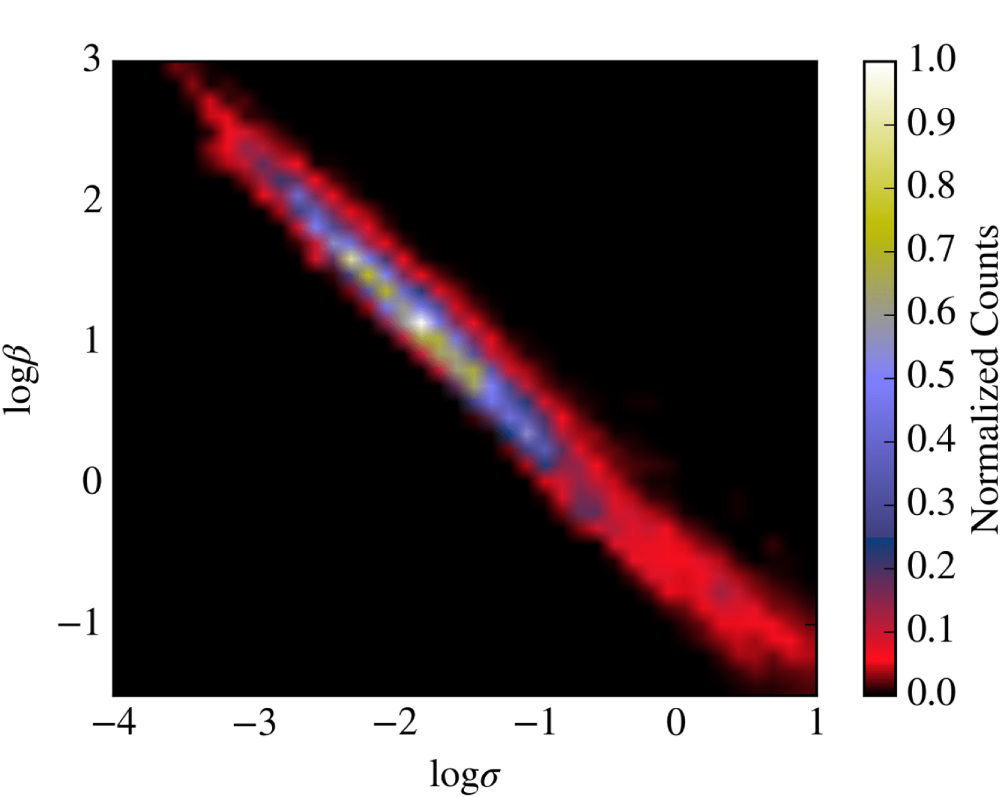
\includegraphics[width =\textwidth]{paper2_fig7.jpg}
	\caption{Two-dimensional histogram of the magnetization $\sigma$ and plasma-$\beta$ across all current sheets in the inner $10 \; GM/c^2$ of the MAD simulation.}
	\label{MAD_hist}
\end{figure}

\begin{figure}[!h]
	\centering
	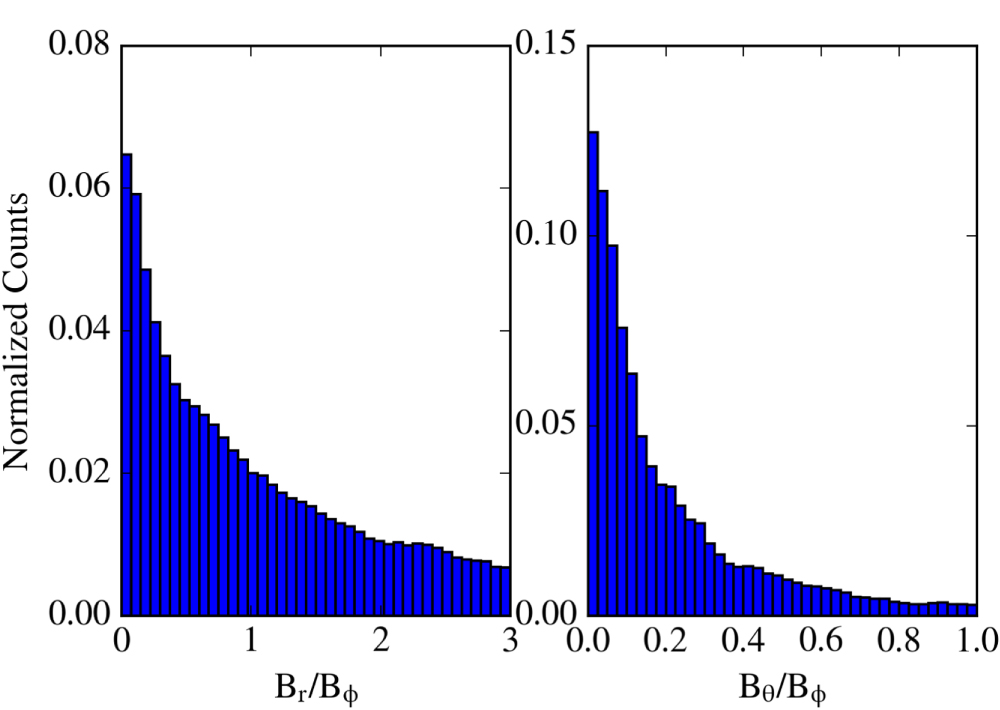
\includegraphics[width =\textwidth]{paper2_fig8.jpg}
	\caption{Histogram of guide fields in the MAD simulation, scaled to $B_{\phi}$, the component showing field reversal. While many sheets have little to no guide fields present, there are a significant number of current sheets with strong guide fields that will likely impact the efficiency of particle acceleration in these sheets.}
	\label{MAD_bguide}
\end{figure}


\section{Variability of Magnetic Energy available for Reconnection}

We finally examine the time variability of energy available to reconnection throughout the accretion flow. One
motivation for this is to assess whether reconnection
events can contribute substantially to the high energy
variability of low luminosity accretion flows, as has been
extensively observed in the case of Sgr A*. We integrate the magnetic energy density, $B^2/8\pi$, over the reconnecting volume bounded by the surfaces defined by
the asymptotic magnetic field location and obtain in this
way the total magnetic energy in the reconnection regions throughout the flow. We plot the results of this in
Figure 8 for both the SANE and MAD simulations.

\begin{figure*}[!h]
	\centering
	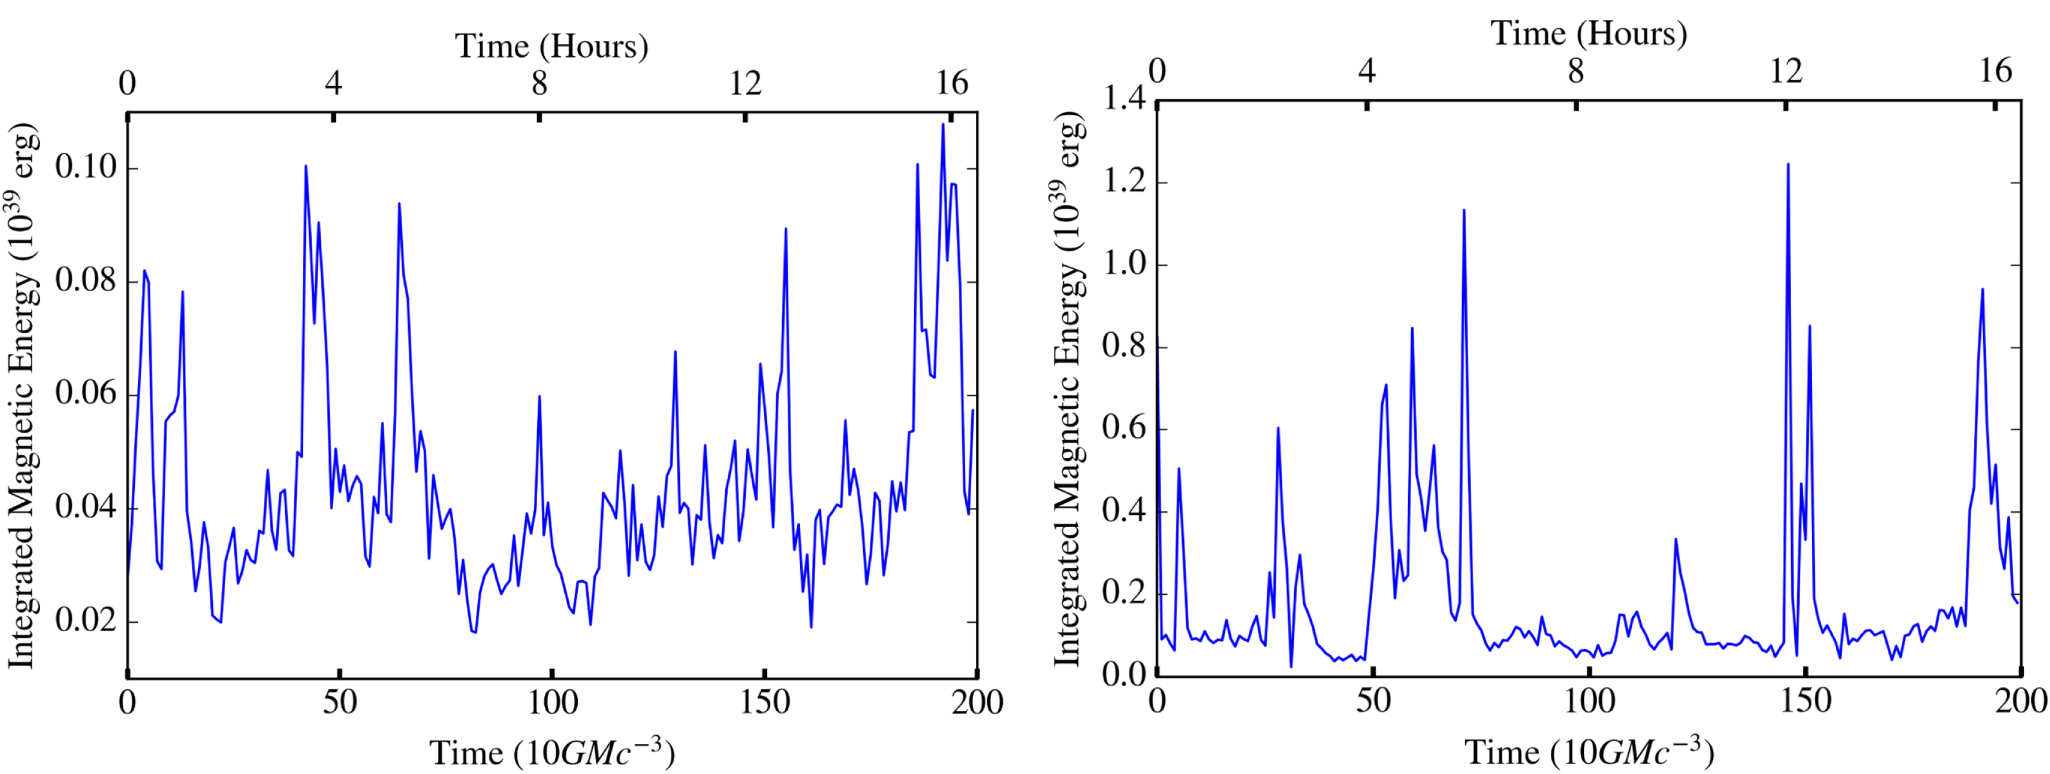
\includegraphics[width=\textwidth]{paper2_fig11.jpg}
	\caption{Magnetic energy of reconnection regions as a function of time in the (left) SANE and (right) MAD simulations. Note the rapid and strong variation over short timescales in both cases, making magnetic reconnection a promising candidate for contributing to the X-ray variability. }
	\label{mag_var}
\end{figure*}

We see that the turbulent nature of the accretion flow
very often leads to the formation of transient current
sheets that result in a highly time-varying magnetic energy being available to reconnection. This indicates that
magnetic reconnection likely is a significant contributor
to the variability of such systems. The SANE model
produces persistent variability due to the high levels of
turbulence in the disk. The MAD system has less turbulence and, hence, fewer variations, but the higher degree
of magnetization means that, when a current sheet does
develop, it typically has more magnetic energy associated
with it. For this reason, we find that the MAD simulation is characterized by fewer but stronger variations in the magnetic energy available to reconnection.

Figure \ref{sig_flare_hist} shows histograms of $\sigma$ for the current sheets of both SANE (left) and MAD (right) simulations, shown at a quiescent and flaring timestep. We see that during times of
increased magnetic energy, there tends to be an associated
population of current sheets with higher-than-typical magnetizations (around $\sigma \approx 1$ for the SANE case, and $\sigma \approx 10$ for MAD). This has significant implications for electron acceleration, because the typical energy of non-thermal electrons, as
well as the efficiency of electron acceleration both scale with $\sigma$.
\begin{figure}[!h]
	\centering
	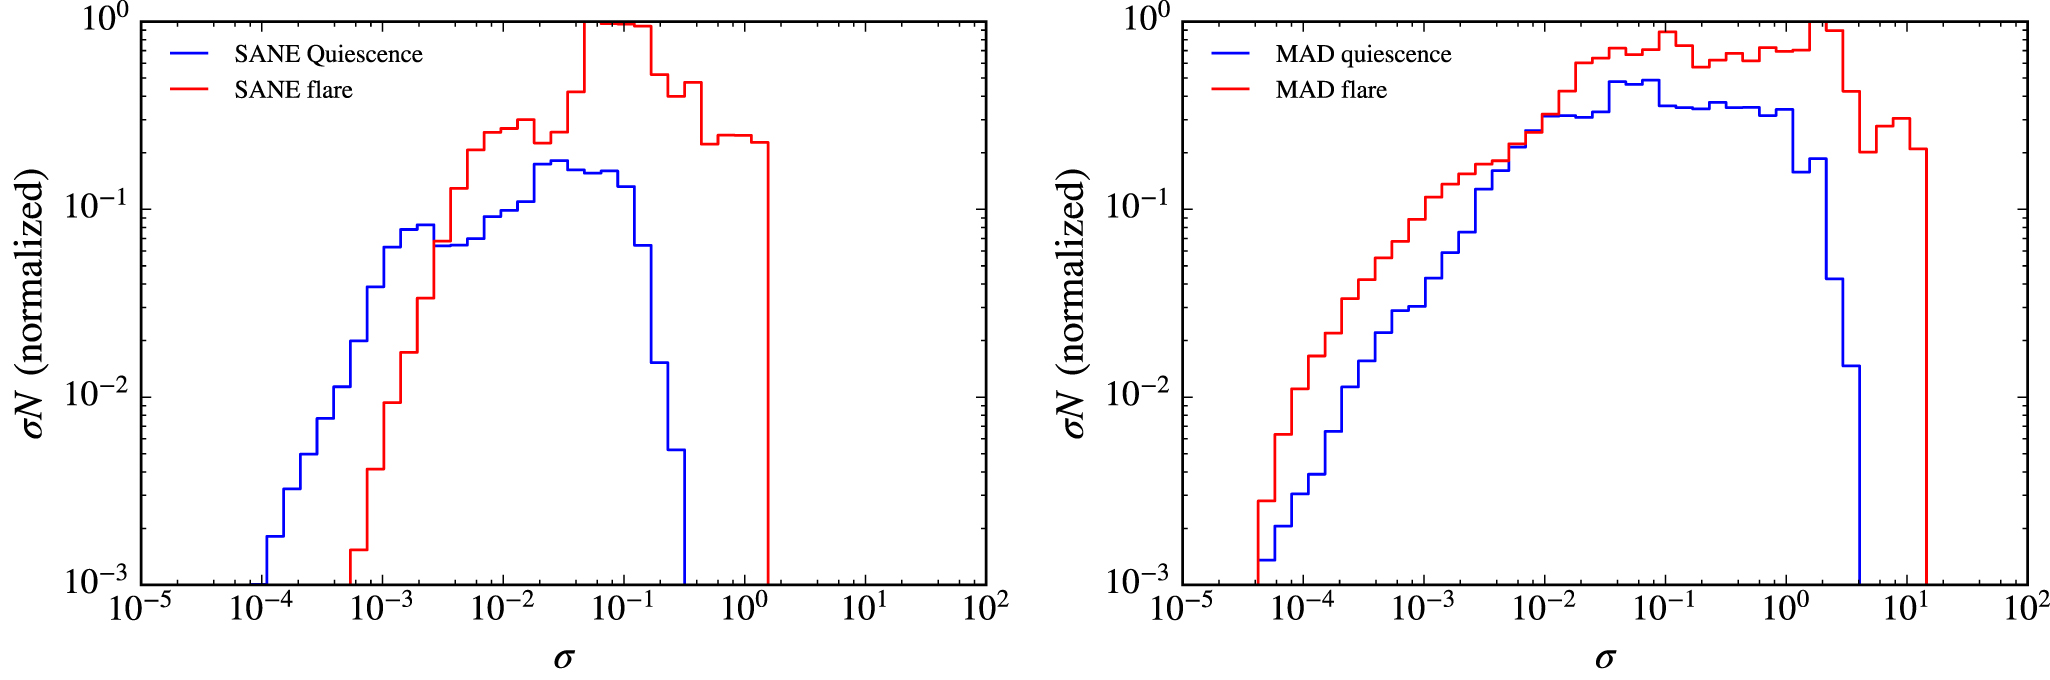
\includegraphics[width =\textwidth]{paper2_fig10.jpg}
	\caption{Histograms of $\sigma$ associated with current sheets in SANE (left) and MAD (right) simulations for both flaring and quiescent timesteps. We see that the increase in magnetic energy during a flaring time is associated with a population of current sheets with higher magnetizations.}
	\label{sig_flare_hist}
\end{figure}
Including the variability properties of non-thermal
electrons that are accelerated in these current sheets will
likely alter significantly the earlier finding of Chan et al.
(2015a), who used models that assumed a purely thermal electron distribution. In that early work, the variability of MAD simulations was characterized by smooth
long timescale variations in the flux. It is clear, however,
from the present analysis of the MAD simulation that
there is the potential for having a sudden injection of
non-thermal electrons associated with the spikes in Figure 5, which can then result in corresponding flares in
the lightcurve.
Based on previous studies, we expect some fraction of
this magnetic energy to go towards accelerating particles.
This acceleration efficiency will, in principle, depend on
the flow conditions, such as $\sigma$ and $\beta$, and can be found
through PIC simulations. In order to go from a picture
such as the one shown in Figure 8 to the non-thermal
particle energy as a function of time, the magnetic energy as a function of time must be combined with the
acceleration efficiency as a function of flow parameters,
which will likely result in even more dramatic variation
of energy on short timescales.
To estimate whether the energy available for reconnection is a plausible explanation for flares of these magnitudes, we calculate the total energy from an average X-ray flare from Sgr A*. Observations of X-ray flares from
Sgr A* show typical luminosities from  $\sim 10^{34}$ $\rm{erg} \rm{s}^{-1}$ to $2  10^{35} \; \rm{erg} \;  s^{-1}$ and typical timescales from hundreds of s to 8 ks (Neilsen et al. 2013). With a luminosity of $5 \times 10^{34} \; \rm{erg} \rm{s}^{-1}$ and a duration of 1000 s, about $5 \times 10^{37} \; \rm{erg}$ is being released in a typical flare.
Considering Figure 8, we see for the SANE model that
the energy available to reconnection peaks at typical values around $10^{38}$ erg, while typical MAD energies are an
order of magnitude higher than this. This shows that
there is enough energy available to reconnection in these
simulations to plausibly account for the observed energy
released during these flares. Moreover, the efficiency $\psi$
that determines the fraction of magnetic energy that goes
into particle acceleration must be quite high in the case
of SANE models, which have typically lower magnetizations and hence less magnetic energy associated with
their current sheets.
In Ball et al. (2016), we characterized the non-thermal
particle distribution using $\eta$, the fraction of non-thermal
to thermal energy densities in the fluid and power-law
index, p. We found that significant X-ray flares can occur
while satisfying the observed quiescent X-ray constraints
for values of $\eta = 0.1$ and a conservative power-law index
of $p = -3.5$. To connect our present results to these
earlier findings, we express $\eta$ in terms of $\beta$ and $\psi$ as
\begin{equation}
	\eta \equiv \frac{E_{nt}}{E_{th}}=\frac{\psi B^2}{nkT8\pi}=\psi \beta^{-1}.
\end{equation}
We can rewrite this as a constraint on the plasma-$\beta$ using the $\eta$ found in our previous study to result in significant X-ray variability, i.e., 
\begin{equation}
	0.1 (\frac{\eta}{0.1}) \beta \leq \psi.
\end{equation}
This places a constraint on the plasma-$\beta$, given a local
$\psi$, which must be found as a function of flow parameters
via PIC simulations. Note that $\psi$, by definition, cannot
be greater than 1, placing a strict upper limit of $\beta = 10$
for regions where there is sufficient magnetic energy to
accelerate particle to the energies required to generate
the flux excursions demonstrated in \citet{ball2016}.
More realistically, $\psi$ is likely to be of order 0.1, resulting
in an upper limit of $\beta \approx 1$. As shown in Figure \ref{label}, we find
that we indeed identify many current sheets satisfying
this condition.

\section{Conclusion}
In this paper, we investigated the detailed structure of
current sheets and their plasma properties in GRMHD
simulations of radiatively inefficient accretion flows. We
found that the regimes of plasma parameters relevant to
magnetic reconnection have been relatively unexplored
in terms of non-thermal particle acceleration. Specifically, we found that the magnetization $\sigma$ in the vicinity
of current sheets in the SANE simulation is of order $10^{-4}$
to $1$ , while the plasma-$\beta$ is of order $0.1$ to $10^3$
. Current sheets in the MAD simulation have magnetization
$\sigma$ ranging from $10^{-3}$
to $1$0 and plasma-$\beta$ from $0.03$ to
$10^3$. Additionally we find that, in these regions, there
is a relatively small spread in temperature, leading to a
tight correlation between the parameters $\sigma$ and $\beta$. We
also characterized the guide fields found in current sheets,
which can play a role in governing the details of particle
acceleration, and found that the ratio of guide field to
reconnecting field strength is typically 0–0.5 for SANE
simulations, but can be of order unity in MAD simulations.
GRMHD simulations need to use subgrid models in
order to account for physical effects that cannot be resolved or incorporated in MHD. In order to employ correctly subgrid models of reconnection, we must improve
our understanding of particle acceleration and heating in
the parameter space we lay out here.
In addition to characterizing the plasma properties of
current sheets, we also calculated the magnetic energy
available to reconnection throughout the simulations.
We found that the turbulent nature of the accretion flow
leads to current sheets of varying characteristics continuously forming and dissipating in the flow. This leads
to a highly variable amount of energy available to reconnect and dissipate into heating and particle acceleration
and makes magnetic reconnection a promising candidate
for contributing to the X-ray variability of Sgr A* and
other black holes with similar accretion characteristics.
Additionally, we found that there is indeed enough energy available to reconnection around current sheets to
account for typical flares observed from Sgr A*. We conclude that if this mechanism is responsible for the X-ray
flares, then the acceleration efficiency must be reasonably high for SANE disks and can be lower for the MAD
model.
\chapter[Electron and Proton Acceleration in Transrelativistic Magnetic Reconnection: Dependence on $\sigma$ and $\beta$]
{Electron and Proton Acceleration in Transrelativistic Magnetic Reconnection: Dependence on $\sigma$ and $\beta$}
\section{Introduction}
%Low-luminosity accretion flows, such as the one at the center of the Milky Way, Sagittarius A* (Sgr A*), are well described by a ``radiatively inefficient accretion flow'' (RIAF).  RIAFs are geometrically thick and optically thin, consisting of a relatively dilute and hot plasma.  Because of the low densities in these disks, the timescale for Coulomb collisions between particles is extremely long, permitting the plasma to exist in a two-temperature state, where the ions and electrons are thermally decoupled.  Additionally, because collisions are so rare, the particle distribution functions are likely to have a significant non-thermal component, which can be generated by various acceleration mechanisms such as shocks, magnetic reconnection, and the dissipation of turbulence.  Non-thermal particle acceleration associated with these plasma processes can only be described in a fully-kinetic framework, and hence are well suited to study via particle-in-cell (PIC) simulations.  The results from PIC simulations can provide subgrid models for magneto-hydrodynamic simulations, in order to account for physics that is not captured in standard fluid theories.

%In \citet{ball2016}, we showed that a localized population of highly energetic non-thermal electrons in a radiatively inefficient accretion flow can generate significant x-ray variability that purely thermal MHD models are unable to reproduce.  Motivated by this study, in \citet{ball2017}, we characterized the properties of current sheets in general-relativistic magneto-hydrodynamic simulations of radiatively inefficient accretion flows, and found that the typical magnetization $\sigma$ of the current sheets are in the trans-relativistic regime $\sigma \approx 1$.  


One of the key parameters that determines the outcome of reconnection and the properties of the resulting particle distribution is the  magnetization of the ambient plasma, i.e., the ratio $\sigma$ of magnetic energy density to enthalpy density. 
%expressed by the parameter $\sigma=B_{0}^{2}/4\pi w_{0}$, where $B_{0}$ is the magnetic field strength in the ambient plasma, and $w_{0}$ is the initial enthalpy density.  
Numerous studies have investigated the non-relativistic ($\sigma\ll 1$) regime, which has applications to the solar corona and solar flares (e.g., \citealt{drake2013}; \citealt{dahlin2014}; \citealt{shay2014}; \citealt{liguo2015}).  The ultra-relativistic ($\sigma\gg 1$) regime has also been explored in detail, due to its relevance to high-energy emission from blazar jets and pulsar wind nebulae (e.g., \citealt{kagan2013}; \citealt{sironi2014}; \citealt{guod_14, guo2015, guo_16}; \citealt{melzani2014}; \citealt{kagan2015}; \citealt{nalewajko2015}; \citealt{werner2016}; \citealt{sironi2016}).  However, only a limited number of studies have been carried out in the trans-relativistic regime ($\sigma \sim 1$), addressing particle heating (\citealt{rowan2017}) and acceleration (\citealt{melzani2014b}; \citealt{werner2018}). The trans-relativistic regime is of particular interest to studies of radiatively inefficient accretion flows around black holes, such as Sgr A* at our Galactic center. Here, current sheets with typical magnetizations of $\sigma\sim1$ are frequently observed in global MHD simulations (\citealt{ball2017}).  Localized particle acceleration powered by magnetic reconnection in these settings could give rise to high-energy variability (\citealt{ball2016}; \citealt{li2017}).  

Earlier investigations (e.g., \citealt{schoeffler2011}; \citealt{schoeffler2013}; \citealt{rowan2017}) have shown that, in addition to the magnetization $\sigma$, the initial plasma temperature, or equivalently the proton $\beta$ (i.e., the ratio of proton thermal pressure to magnetic pressure), can affect the dynamics and energetics of magnetic reconnection.  In particular, \citet{rowan2017} explored the dependence of the electron and proton heating efficiency on the magnetization $\sigma$, the proton $\beta$, and the electron-to-proton temperature ratio.  However, the role of $\beta$ on non-thermal particle acceleration in the trans-relativistic regime ($\sigma\sim1$) remains largely unexplored. 

The works by \citet{melzani2014b} and \citet{melzani2014} were the first to investigate particle acceleration in the trans-relativistic regime of reconnection. They examined the energy partition between protons and electrons and the electron power-law spectra, but they employed a reduced proton-to-electron mass ratio, and they only explored a relatively narrow range of $\beta$. \citet{werner2018} performed an extensive study across a wide range of $\sigma$, from the trans-relativistic through the ultra-relativistic regime, and reported how the reconnection rate, the electron power-law slope, and the energy partition between electrons and protons depend on $\sigma$.  They found that the electron power-law slope decreases with increasing $\sigma$ (so, the spectrum hardens) and provided an empirical fit $p\simeq1.9+0.7/\sqrt{\sigma}$ for the power-law slope $p$ of the electron spectrum.  However, their study was performed at a fixed value of proton beta $\beta=0.01$.  

 %This study is the first to systematically map out the details of particle acceleration in the transition from the trans-relativistic to the ultra-relativistic regimes.  


%Given the importance of $\sigma$ and the plasma-$\beta$ in the outcome of particle acceleration and heating from magnetic reconnection, PIC studies aim to map out the dependence of the final particle energy spectra across this parameter space. 
In this work, we investigate proton and electron non-thermal acceleration in trans-relativistic  reconnection, covering the whole parameter space in $\sigma$ and $\beta$ and employing the physical proton-to-electron mass ratio. For four values of the magnetization ($\sigma=$ 0.1, 0.3, 1, and 3), we explore a wide range of $\beta$, from $\beta=10^{-4}$ up to the maximum possible value of $\beta$, that is $\beta_{\rm max}\approx 1/4\sigma$ (we will discuss why this is the maximum in Section \ref{setup}). Our study goes beyond the current state of the art in several respects: we explore for the first time the dependence of the non-thermal electron spectrum on  plasma $\beta$, and we examine the role of various electron acceleration mechanisms, by tracking particles in our simulations. In addition, our computational domains are larger than previous works by at least a factor of $\sim5$.
While we primarily focus on electrons, we also present proton spectra and briefly investigate proton acceleration mechanisms.

We find that the electron spectrum in the reconnection region can be generally modeled as a non-thermal power law, but the properties of the spectrum are strongly dependent on $\beta$. At $\beta \lesssim 3 \times 10^{-3}$, the spectrum is dominated by a hard power law, whose slope is insensitive to $\beta$ and depends on $\sigma$ as $p\simeq 1.8 +0.7/\sqrt{\sigma}$, in agreement with the result by \citet{werner2018}. The electron spectrum tends to steepen for larger simulation domains. Electrons are primarily accelerated by the non-ideal electric field at X-points, either  in the initial current layer  or in current sheets generated in between merging magnetic islands. 
At higher $\beta$, the electron power law steepens significantly, and the electron spectrum eventually approaches a Maxwellian distribution, for all values of $\sigma$. At high values of $\beta$ near $\beta_{\rm max}\approx1/4\sigma$, when both electrons and protons start relativistically hot, the spectrum of both species displays an additional component at high energies, containing a few percent of particles, which are accelerated via a Fermi-like process by bouncing in between the reconnection outflow and the stationary magnetic island at the boundary of our periodic domain.
We investigate the dependence of our results on the size of the simulation domain, finding that  the high-energy  cutoff of the electron spectrum increases with box size. 
For the main population of non-thermal electrons (i.e., excluding the additional component emerging at $\beta\rightarrow \beta_{\rm max}$),
we provide an empirical prescription for the dependence of the power-law slope and the acceleration efficiency on $\beta$ and $\sigma$. The results of our study can be used as subgrid models in global MHD simulations of  black hole accretion flows (e.g., \citealt{ball2016}; \citealt{mao2017}; \citealt{chael2017}), potentially unveiling the origin of the flaring behaviour of Sgr A* \citep{ponti17}.

The layout of the paper is as follows.  In Section \ref{setup} we describe the setup of our simulations.  In Section \ref{time_evol}, we show and describe the time evolution of a representative simulation and the evolution of its associated electron and proton energy spectra.  In Section \ref{role_of_beta}, we explore the dynamics of the reconnection layer as a function of $\sigma$ and $\beta$, and illustrate the key differences between low- and high-$\beta$ reconnection.  In Section \ref{energy_spectra}, we show the electron and proton spectra for a number of values of $\sigma$ and $\beta$, and provide an empirical fit to the electron power-law slopes and acceleration efficiencies.  Finally, in Section \ref{mechanism}, we show representative trajectories of accelerated electrons for both a low-$\beta$ and a high-$\beta$ simulation.  We conclude and summarize in Section \ref{conclusions}.

\section{Simulation Setup}\label{setup}
We perform a large suite of PIC simulations of anti-parallel magnetic reconnection using the  publicly-available code TRISTAN-MP (\citealt{buneman93}; \citealt{spitkovsky05}).  We employ a two-dimensional (2D) simulation domain in the $xy$ plane, but we track all three components of velocity and electromagnetic field vectors.  We set up the system in Harris equilibrium, with a magnetic field profile $\bm{{B}} = -B_{0}\tanh{\left(2\pi y / \Delta\right)}\bm{\hat{x}}$, where $B_{0}$ is the strength of the reconnecting field in the ambient plasma and $\Delta$ is the thickness of the sheet.  $B_{0}$ is related to the magnetization parameter $\sigma$ via $\sigma=B_{0}^2 / 4\pi w_{0} $, where $w_{0}$ is the enthalpy density of the ambient plasma $w_0=(\rho_{e}+\rho_{i})c^{2}+ \hat{\gamma}_{e}u_{e}+ \hat{\gamma}_{i}u_{i}$, with $\rho_{i,e}$, $\hat{\gamma}_{i,e}$, and $u_{i,e}$ being the mass densities, adiabatic indices, and internal energy densities of ambient protons and electrons, respectively.  The temperature is specified through the proton $\beta$, defined as $\beta \equiv \beta_{i}=8 \pi n_{i} k T_{i}/B_{0}^{2}$, where $n_i=\rho_i/m_i$ is the proton number density, $T_i$ is the proton temperature, and $m_i$ is the proton mass. Ambient electrons and protons start with the same temperature, so $\beta_e=\beta_i=\beta$ (the total plasma beta, including both species, is $2\,\beta$). In most cases, the ambient protons are non-relativistic, so the magnetization parameter as defined with the proton rest mass $\sigma_i=B_0^2/4\pi \rho_i c^2$ is nearly identical to the enthalpy-weighted magnetization $\sigma$ defined above. Each computational cell in the ambient plasma is initialized with four particles per cell (so, $N_{ppc}=4$), but we have tested that our results are the same when using $N_{ppc}=16$ (see Appendix \ref{convergence}).

The thickness of the current sheet is $\Delta = 80 \,c/\omega_{p}$, where $\omega_{p}$ is the electron plasma frequency, given by 

\begin{equation}
\omega_{p} =\sqrt{\frac{4\pi n_{e}e^{2}}{m_{e}}}\left(1+\frac{\theta_{e}}{\hat{\gamma_{e}}-1}\right)^{-1/2}.
\label{electron skin depth}
\end{equation}
Here, $e$ is the electron charge, $m_e$ is the electron mass, $n_e=\rho_e/m_e$ is the electron number density ($=n_i$) and $\theta_{e}$ is the dimensionless electron temperature $\theta_{e}=kT_{e}/m_{e}c^{2}$ in the ambient plasma. 
We set up the initial Harris equilibrium by initializing the plasma in the current sheet to be hot and overdense (by a factor of 3 with respect to the background) so that its thermal pressure balances the magnetic pressure outside the sheet. The particles in the current sheet are set up as a Maxwellian distribution drifting in the $z$ direction, so that their electric current balances the curl of the magnetic field. 

Our computational domain is periodic in the $x$-direction of the reconnection outflow (in order to retain all accelerated particles), while the box is continually enlarged in the $y$-direction, as two moving injectors --- that steadily inject magnetized plasma into the simulation domain --- recede from the current sheet at the speed of light along $\pm\bm{\hat{y}}$. By employing the moving injectors and a dynamically-enlarging box (see \citealt{sironi2009} for further details), we can study the late-time evolution of the system without being artificially limited by the finite amount of plasma and magnetic flux that is initially in the simulation domain. Additional computational optimization is achieved by allowing the injectors to periodically ``jump'' back towards the current sheet, removing all particles beyond the injectors and resetting the electromagnetic fields to their initial values.

The length of the box in the $x$ direction of the reconnection outflow is $L_x=16620$ cells, which corresponds to $L_x\simeq5540\,c/\omega_{p}$, since we resolve the electron skin depth $c/\omega_{p}$ with 3 computational cells. As described in Appendix \ref{convergence}, we have tested that our results are the same when the electron skin depth is resolved with 6 cells. We also investigate the dependence of our results on the extent $L_x$ of the computational domain (up to a factor of two larger than our reference runs), see Appendix \ref{boxsize}.

We trigger reconnection in the center of the box by removing by hand the pressure of the hot particles initialized in the center of the sheet (see \citealt{sironi2016}).  This causes the current sheet to collapse and form two ``reconnection fronts,'' which are pulled by magnetic tension along $\pm \bm{\hat{x}}$ at roughly the Alfv\'en speed $v_{A}=c\sqrt{\sigma/(1+\sigma)}$.  We define the Alfv\'enic crossing time as  $t_{A} = L_{x}/v_{A}$.  At $t\gtrsim 0.5\,t_A$, the reconnected plasma starts accumulating at the boundary of the periodic simulation domain, where a ``boundary island'' forms.

Astrophysical current sheets are likely thick, making the timescale for spontaneous (or ``untriggered'') reconnection very long compared to relevant dynamical timescales.  This means that astrophysical reconnection is likely triggered by some large-scale perturbation, which motivates our decision to trigger reconnection in our simulations. In fact, the large-scale perturbation will induce a curvature of the field lines over a scale $\sim L_x$, such that the current sheet is narrower near the center. The central region is then most likely to go unstable via the tearing mode, and the signal of ongoing reconnection will propagate toward the outer regions (where the current sheet is broader) before they have time to spontaneously become unstable. We further discuss our choice of a triggered setup in  Appendix \ref{untriggered}, where we compare our results to the case of untriggered reconnection, where the  system goes unstable via numerical noise, as in \citealt{sironi2014}. In Appendix \ref{untriggered}, we also compare the results of triggered simulations with either periodic or outflow boundaries in the $x$ direction (for further details on the implementation of the outflow boundary conditions, see \citealt{sironi2016}).


\begin{deluxetable}{ccccccc}
\centering
\tablewidth{1\columnwidth}
\tablecaption{Simulation Parameters}  
\tablehead{run&$\sigma$& $\sigma_{i}$ & $\beta$ & $L_{x}$ ($c/\omega_{pi}$) &$L_{x}$ ($r_{e,\rm hot}$) &$kT_{i}/m_{i}c^{2}$}
\startdata
A0& 0.1 & 0.1& $1\times 10^{-4}$ & 125 & 406&$5 \times 10^{-6}$\\ 
 \hline
A1& 0.1 & 0.1& $3\times 10^{-4}$ & 127 & 417&$1.5 \times 10^{-5}$\\ 
 \hline
A2& 0.1& 0.1 & $10^{-3}$ & 134& 453 & $5 \times 10^{-5}$\\
 \hline
A3& 0.1& 0.1 & $3\times 10^{-3}$ & 158 & 542 & $1.5 \times 10^{-4}$\\
 \hline
A4& 0.1& 0.1 & 0.01  & 233& 776 & $5 \times 10^{-4}$\\
 \hline
A5&  0.1 & 0.1& 0.02& 312 & 1020& $1 \times 10^{-3}$\\
 \hline
A6&  0.1 &  0.1 &0.1 & 664& 2110 & $5 \times 10^{-3}$\\
 \hline
A7 & 0.1& 0.11 & 0.3 & 1138 & 3978& 0.02\\
 \hline
A8& 0.1 &0.16& 1.5  & 4133& 7269 & 0.1\\ %[1ex] 
 \hline
B0 & 0.3&0.3 & $1\times 10^{-4}$ & 127& 241&$1.5\times 10^{-5}$\\ 
 \hline
B1 & 0.3&0.3 & $3\times 10^{-4}$  & 134& 261&$5\times 10^{-5}$\\ 
 \hline
B2& 0.3&0.3 & $10^{-3}$  & 156& 313&$1.5\times 10^{-4}$\\
  \hline
B3& 0.3&0.3 & $3\times 10^{-3}$ & 232& 448&$5\times 10^{-4}$\\
 \hline
B4& 0.3&0.3 & $6\times 10^{-3}$ &312& 589 &$1\times 10^{-3}$\\
 \hline
B5& 0.3&0.3 & 0.01 &375& 701&$1.5\times 10^{-3}$\\
 \hline
B6&  0.3&0.3 & 0.03 & 664& 1218&$5\times 10^{-3}$\\
 \hline
B7&  0.3 & 0.34&0.11 & 1138& 2296&0.02\\
 \hline
B8*& 0.3&0.72 & 0.55 & 4133& 4956&0.2\\ %[1ex] 
 \hline
C0&  1 &1& $1\times 10^{-4}$ & 134& 143&$5 \times 10^{-5}$\\ 
 \hline
C1&  1 &1& $3\times 10^{-4}$ & 157& 171&$1.5 \times 10^{-4}$\\ 
 \hline
C2& 1 &1& $10^{-3}$  &232& 245&$5 \times 10^{-4}$\\
 \hline
C3& 1 &1& $3\times 10^{-3}$ & 375& 384&$1.5 \times 10^{-3}$\\
 \hline
C4& 1 &1& 0.01 & 664& 667&$5 \times 10^{-3}$\\
 \hline
C5& 1&1.1 & 0.03 & 1138& 1107& 0.015\\
 \hline
C6& 1&1.3 & 0.08  & 2069& 1827& 0.05\\
 \hline
C7*& 1&2.4 & 0.16 & 4133& 2713&0.2\\
  \hline
D0&  3&3 & $10^{-4}$ & 157& 99 & $1.5 \times 10^{-4}$\\ 
 \hline
D1& 3 &3& $3\times 10^{-4}$ & 232& 141& $5 \times 10^{-4}$\\ 
 \hline
D2& 3 &3& $10^{-3}$ & 375& 221& $1.5 \times 10^{-3}$\\
 \hline
D3& 3 &3.1& $3\times 10^{-3}$ & 664& 385& $5 \times 10^{-3}$\\
 \hline
D4& 3&3.3 & 0.01 & 1138& 639&0.015\\
 \hline
D5*&  3&4.0 & 0.026 & 2069& 1055&0.05\\
 \hline
D6*&  3 &7.2 &0.055  & 4133& 1566&0.2
  %\hline
\enddata
\tablecomments{Summary of the physical and numerical parameters of our simulations.  All simulations are performed with the physical mass ratio, equal electron and proton temperatures, a resolution of 3 cells per electron skin depth, and 5,440 electron skin depths along the current layer.}
\label{tab:fit}
\end{deluxetable}

The physical and numerical parameters of our simulations are summarized in Table 1. To fully map out the parameter space of interest, we perform 33 simulations across four different values of the magnetization: $\sigma=\,$0.1, 0.3, 1, and 3. For each value of $\sigma$, we have multiple (at least 7) simulations in which we vary the proton $\beta$ from $10^{-4}$ up to the maximum possible value of $\beta$, $\beta_{\rm max}\approx 1/4\sigma$. This upper limit in $\beta$ is reached when both protons and electrons become relativistically hot. In this limit, the internal energy densities dominate over the rest mass energy densities, so the enthalpy density is  $w_0\simeq \hat{\gamma}_{e}u_{e}+\hat{\gamma_{i}}u_{i}$. For $\hat{\gamma}_{e}=\hat{\gamma}_{i}=4/3$, as appropriate for a 3D ultra-relativistic gas, the magnetization tends to $\sigma \simeq 1/4\beta$, which defines an upper limit on $\beta$ at a given $\sigma$, equal to $\beta_{\rm max}\approx 1/4\sigma$.


Due to computational constraints, PIC codes often employ a reduced proton-to-electron mass ratio, in order to decrease the separation of scales between the two species. However, as we have shown in  \citealt{rowan2017}, a choice of the mass ratio smaller than the physical one can artificially affect the partition of energy between electrons and protons in trans-relativistic reconnection. Since it could also artificially affect the efficiency and slope of non-thermal particle acceleration, in this study we employ the physical mass ratio $m_{i}/m_{e}=1836$. While the box length $L_x$ measured in electron skin depths is independent of $\beta$ or $\sigma$, the box length in proton skin depths $c/\omega_{pi}$, where
$$
\omega_{pi} =\sqrt{\frac{4\pi n_{i}e^{2}}{m_{i}}}\left(1+\frac{\theta_{i}}{\hat{\gamma_{i}}-1}\right)^{-1/2},
$$ 
varies significantly with $\beta$ due to the $\theta_e$-dependent correction in Equation \ref{electron skin depth}.  For most of our simulations, electrons start as ultra-relativistically hot, while protons are non-relativistic (our maximum $\theta_{i}=kT_i/m_i c^2$ is 0.2, see Table 1).  As  $\beta$ increases, the separation of electron and proton scales decreases, so our domain is effectively larger (in units of the proton skin depth) at higher $\beta$ (see Table 1). In Table 1, we also quote the extent of our simulation domain in units of $r_{e,\rm hot}=\sigma_e m_e c^2/eB_0$ (the unit of length employed by \citealt{werner2018}), which corresponds to the Larmor radius of a relativistic electron with Lorentz factor $\sigma_e=\sigma_i m_i/m_e$.



\begin{figure}[!h]
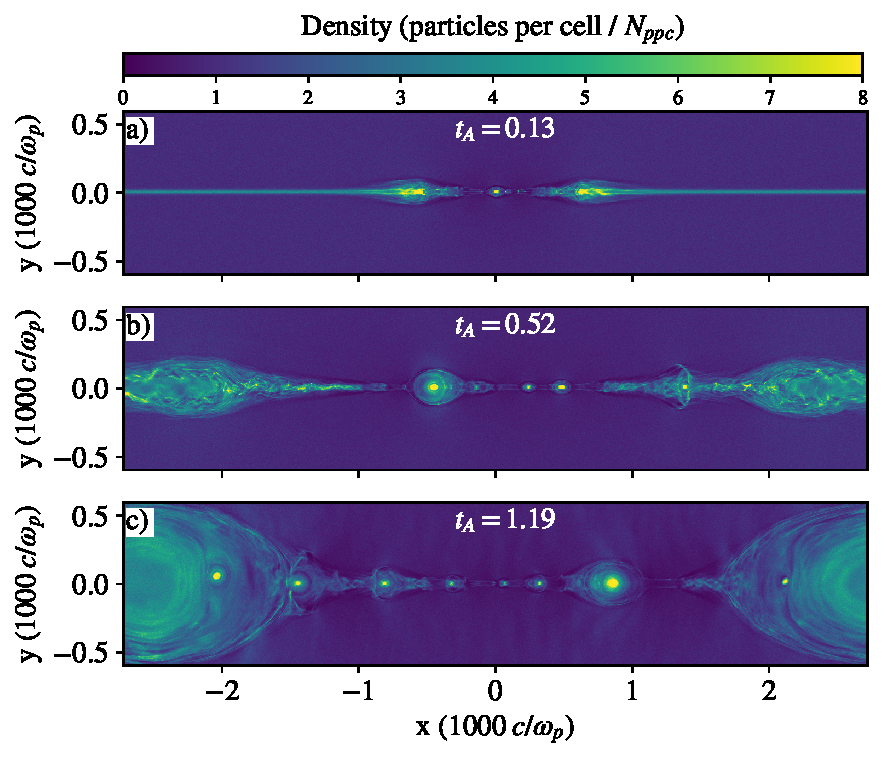
\includegraphics[width=1.0\linewidth]{testing_threeplot.pdf}
\caption{2D snapshots of density depicting the time evolution from a simulation with $\sigma=0.3$ and $\beta=3\times 10^{-4}$ (run B1) at three different times.  The top, middle, and bottom panels correspond to 0.13, 0.52, and 1.19 Alfv\'en crossing times, respectively.  We normalize the density to the initial number of particles per cell in the ambient plasma, $N_{ppc}$.  We scale the density to the power of $0.3$ to enhance the contrast in color scale.}
\label{lowbeta_threeplot}
\end{figure}

\section{Time Evolution of the reconnection layer}\label{time_evol}
In order to illustrate the time evolution of a typical simulation, we show in Figure \ref{lowbeta_threeplot} a series of 2D snapshots of the particle number density for a run with $\sigma=0.3$ and $\beta=3\times10^{-4}$. The lack of pressure support in the vicinity of the center, resulting from our initial perturbation, triggers the collapse of the current sheet (top panel in Figure \ref{lowbeta_threeplot}) and the formation of an X-point. In the following, we shall indicate this X-point as the ``primary X-point.'' While in untriggered systems the tearing mode instability pinches the current sheet at several locations, thus producing several primary X-points, in our triggered setup we only have one primary X-point. The top panel also shows the two reconnection fronts (at $x \approx \pm 500\, c/\omega_{p}$) that are pulled towards the edges of the box by the tension of the magnetic field lines.  In the underdense region in between these fronts, a secondary plasmoid begins to form close to the center, as plasma flows in from above and below the  reconnection layer.  

In the middle panel of Figure \ref{lowbeta_threeplot}, the reconnection fronts are approaching the edges of the box, and numerous secondary plasmoids have formed in the layer, separated by secondary X-points (see e.g., \citealt{loureiro2007}; \citealt{uzdensky2010}; \citealt{huang2012}; \citealt{takamoto2013} and \citealt{comisso2016} for the physics of secondary plasmoid formation).  By ``secondary plasmoids,'' we are referring to structures that form after the early collapse of the current sheet, and that contain particles that belong to the ambient plasma (as opposed to the hot population of particles initialized in the current sheet). A secondary X-point is present in between each pair of neighboring secondary plasmoids. 
The largest plasmoid near the center of the box, at $x\simeq-300 \; c/\omega_{p}$, is formed via mergers of several smaller plasmoids, and contains the highest energy particles in the system at this time (see \citealt{sironi2016} for a discussion of the correlation between plasmoid size and  maximum particle energy).  

In the final snapshot (bottom panel in Figure \ref{lowbeta_threeplot}), the outflowing fronts collide across the periodic boundaries, forming a large magnetic island which sits passively at the edge and acts as a reservoir for accelerated particles. In the following, we shall refer to this structure as the ``boundary island,'' and by ``plasmoids'' we will only mean secondary islands. Secondary plasmoids forming in the sheet are eventually advected into the boundary island by the  tension of the field lines.   A current sheet forms at the interface between the boundary island and each secondary plasmoid that is merging into it. As we will show in Section \ref{mechanism}, this interface is a site of efficient electron acceleration.




\subsection{Defining the Reconnection Region}
The spectrum from the entire simulation domain includes both pre- and post-reconnection plasma.  Because of this, it is prudent to have a scheme to distinguish between particles that have undergone reconnection, and particles that are still in the colder upstream region.  This is an important step to correctly interpret the spectra, and avoid mistaking for a power-law component the ``bridge'' between the pre- and post-reconnection distributions.
In order to extract the spectrum of the plasma that has undergone reconnection, uncontaminated by the cold upstream plasma, we use a mixing criterion to identify regions where reconnection has occurred (as first proposed in \citealt{daughton2014}, and described in \citet{rowan2017}).  In short, we tag particles with an identifier that specifies whether they were initialized above or below the current sheet.  We can then identify the cells where particles have mixed to a sufficient degree and in doing so, define the ``reconnection region'', predominantly populated by particles that have been processed by reconnection.   We take a mixing fraction of one part in 100 as our lower limit to define this region.  Using this technique, we are able to cleanly separate the particles that are part of a region that has undergone reconnection from the colder upstream plasma. For the remainder of this paper, any reference to the ``reconnection region'' refers to the region defined by this criterion.  We show in Figure \ref{regions} the result of applying this method to the snapshot shown in the bottom panel of Figure \ref{lowbeta_threeplot}.  We see that the reconnection region (yellow) is cleanly separated from the upstream plasma (dark purple).

\begin{figure}[!h]
	\centering
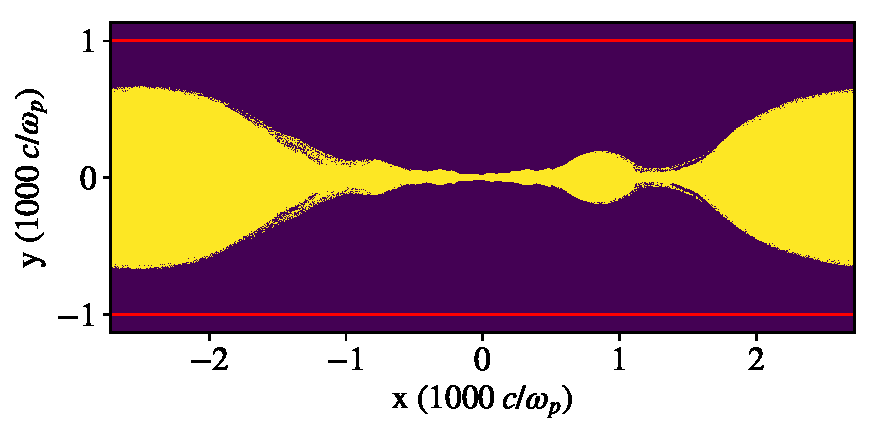
\includegraphics[width=\linewidth]{regions_test.pdf}
\caption{Reconnection region (yellow) identified based on the mixing criterion described in the text. The snapshot refers to the same simulation shown in Figure \ref{lowbeta_threeplot} ($\sigma=0.3$, $\beta=3\times 10^{-4}$, B1), at the last time shown (bottom panel in Figure \ref{lowbeta_threeplot}).  We see that our mixing criterion properly isolates the reconnected overdense plasma from the cold upstream plasma.  The red lines delimit the region in which the total spectra are calculated, as we will discuss in Figure~\ref{timespec}.}
\label{regions}
\end{figure}


\begin{figure}[htp]
	\centering
%\subfloat[Time evolution of the electron energy spectrum (black to red) in  the simulation shown in Figure 1.  The late-time ion energy spectrum is shown in cyan.  ]
{
	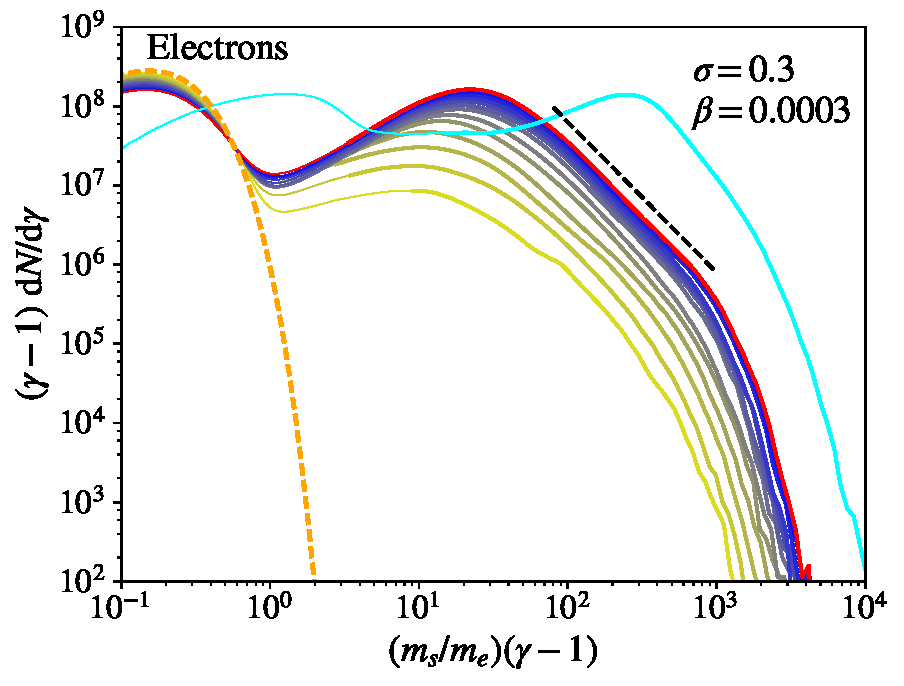
\includegraphics[width=.5\linewidth]{sig_3_delgam00005_timespec.pdf}
}
%\newline
%\subfloat[Time evolution of ion spectra.]
{
	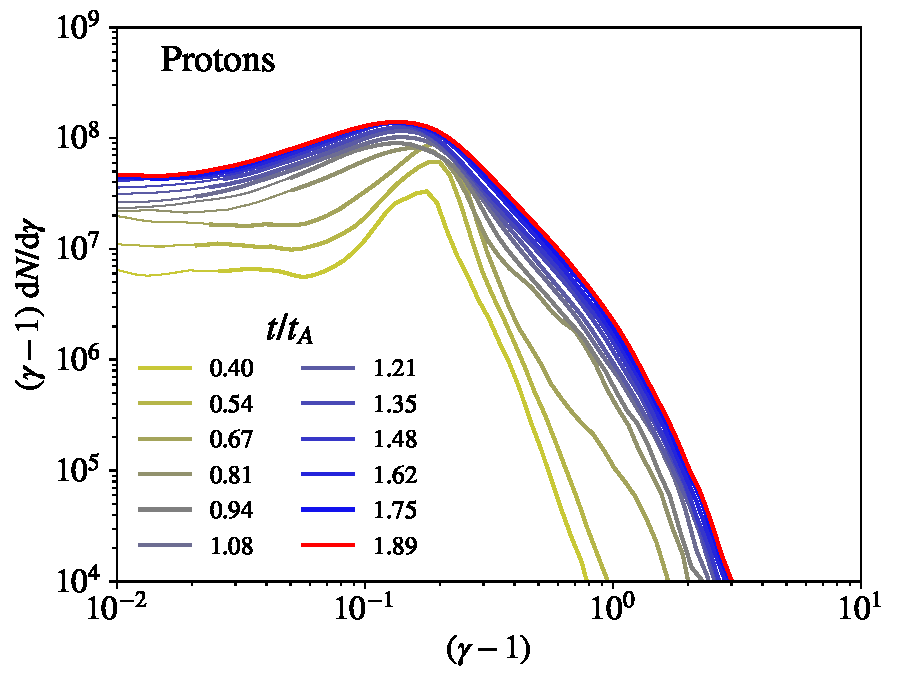
\includegraphics[width=.5\linewidth]{sig_3_delgam00005_timespec_ions.pdf}
}
\caption{Time evolution of the electron (top) and proton (bottom) energy spectra for the simulation shown in Figure \ref{lowbeta_threeplot}, with $\sigma=0.3$ and $\beta=3\times10^{-4}$ (run B1), corresponding to an initial proton thermal spread of $\theta_{i}=5 \times 10^{-5}$. The time sequence (from yellow to blue, with red marking the final time) is indicated in the bottom panel, in units of the Alfv\'enic crossing time $t_A=L_x/v_A$. In each panel, thicker lines indicate the energy range where the spectrum is mostly contributed  by particles in the reconnection region (by more than 75\%). In the top panel, the dashed orange line shows the initial electron Maxwellian for comparison, and the dashed black line represents a power law with slope $p=-d\log{N}/d\log{\gamma}=2.9$.
In the top panel, the proton spectrum at the final time (i.e., red curve in the bottom panel) is overplotted in cyan for comparison, with the horizontal axis rescaled by $m_i/m_e$. Since $m_s=m_e$ for electrons and $m_s=m_i$ for protons, the horizontal axis in the top panel represents the kinetic energy of each species, in units of the electron rest mass.}
\label{timespec}
\end{figure}

\subsection{Time Evolution of the Energy Spectra}
Having seen how the density evolves with time, and where and when various structures such as plasmoids and X-points form, we now examine the time evolution of the electron and proton energy spectra from the same simulation shown in Figure \ref{lowbeta_threeplot}.  We present the time evolution of the electron and proton spectra in the top and bottom panels of Figure \ref{timespec}, respectively. For both species, our spectra only include the particles that start in the ambient plasma (i.e., we exclude the contribution of the hot population that we set up in the current layer, whose properties depend on the initialization of the Harris sheet).  At each time, the spectrum includes all the particles in a fixed region, whose thickness is $\approx 0.2 L_{x}$ on each side of the current  sheet (bounded by the red lines in Figure \ref{regions}). On each curve, a thicker line with the same color marks the energy range where the fractional contribution of the reconnection region (i.e., the yellow region in Figure \ref{regions}) to the overall spectrum is greater than 75\%. So, the sequence of thick lines illustrates the time evolution of the spectrum in the reconnection region (which, from now on, we call ``post-reconnection spectrum'').

In the top panel,  we present the evolution of the electron spectrum, that shows two components. The bump peaking at $\gamma-1 \approx 0.2$ is populated by the cold upstream electrons, and in fact this component is well fit by a Maxwellian distribution with the  temperature that we employ to initialize ambient electrons (dashed orange line). The high-energy component, that peaks at $\gamma \approx 20$, is populated by particles that have been processed by reconnection (in fact, it is plotted with thicker lines, indicating that it is dominated by particles belonging to the reconnection region). The high-energy component is consistent with a single non-thermal population having a power-law slope of $p=-d\log{N}/d\log{\gamma}=2.9$ (as indicated by the dashed black line), that extends from the peak at $\gamma \approx 20$ up to $\gamma\approx1000$, where it cuts off exponentially. The power law starts right at the peak of the high-energy component, a common feature of magnetic reconnection (\citealt{sironi2014}; \citealt{melzani2014b, melzani2014}; \citealt{cerutti2012, cerutti2014, cerutti2017}; \citealt{guo2015}; \citealt{liguo2015};  \citealt{werner2018}). The power-law index is established early on in the evolution of the electron energy distribution, and it does not appreciably change from $t=0.67\,t_{A}$ up to $t=1.89\,t_{A}$. The high-energy cutoff of the electron power law  steadily increases as larger plasmoids form and merge with each other or with the boundary island \citep{sironi2016}. 

In the bottom panel of Figure~\ref{timespec}, we show the time evolution of the proton energy spectrum.  The proton spectrum in the reconnection region resembles a power law at late times, similarly to the electron spectrum. In the top panel, the proton spectrum at the final time ($t=1.89\,t_{A}$) is shown with a cyan line, with the horizontal axis scaled by $m_i/m_e$ in order to compare with the electron spectrum (so, the horizontal axis indicates the kinetic energy of both species, in units of the electron rest mass energy). By comparing the thick cyan line (for protons) with the thick red line (for electrons), we see that the proton mean energy in the reconnection region  is about an order of magnitude larger than the electron mean energy (see \citealt{rowan2017} and \citealt{werner2018} for a discussion of electron and proton heating in trans-relativistic reconnection). We also find that the proton spectrum in the reconnection region has a steeper slope than the electron spectrum, and it spans a smaller range of energies.

The most dramatic difference between electron and proton spectra, though, is in their temporal evolution. At early times, the proton spectrum in the reconnection region (thick lines in the bottom panel) is nearly monochromatic, with a pronounced peak at $\gamma-1 \approx  0.15 \approx  \sigma/2$, as expected from the characteristic kinetic energy of reconnection outflows (moving at $\sim v_A\sim c \,\sqrt{\sigma}$). Starting at $t\approx0.8\,t_A$, the spectrum develops a power-law-like tail. This transition occurs around the time when the two reconnection fronts interact across the periodic boundaries (at a time in between panels (b) and (c) of Figure \ref{lowbeta_threeplot}), forming the large boundary island. This suggests that the interface between the reconnection outflows and the boundary island might be a promising source of non-thermal proton acceleration, as we further discuss in Section \ref{mechanism}. We remark that the development of a non-thermal proton distribution is not a peculiar consequence of our choice of triggering reconnection at the center of our domain. We observe the same evolution of the proton spectrum in untriggered runs, where the tearing mode is allowed to grow spontaneously.

In summary, protons develop a non-thermal tail only after $t\approx0.8\,t_A$, when the two reconnection fronts interact across the periodic boundaries. In contrast, electrons display a non-thermal component since early times. Although we only show here one particular choice of $\sigma$ and $\beta$, this trend holds across all of our low-$\beta$ simulations (the cases with $\beta$ approaching $\beta_{\rm max}$ are an exception, as we discuss below). These differences between the temporal evolution of electron and proton spectra point towards different acceleration mechanisms for the two species, as we discuss further in Section \ref{mechanism}. In particular, we will show that in low-$\beta$ cases, electrons are significantly accelerated at their first interaction with the layer by the non-ideal electric field at X-points. The early evidence for non-thermal electrons then comes from the fact that X-points appear since the earliest stages of evolution of the layer (see Figure \ref{lowbeta_threeplot}).

\begin{figure}[!h]
	\centering
	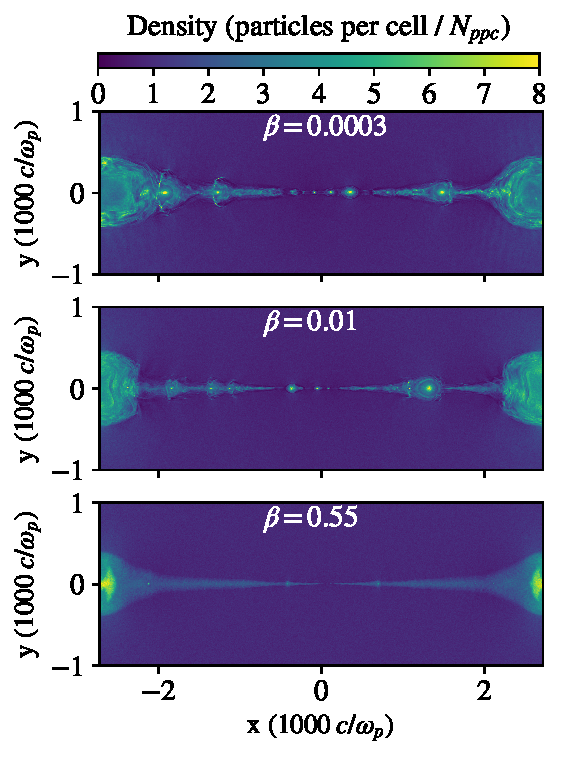
\includegraphics[width =0.5\textwidth]{sig_3_threeplot.pdf}
	\caption{2D density structure  at $t\approx t_{A}$ for a suite of simulations with fixed $\sigma=0.3$ and varying $\beta$: $\beta=0.0003$ (top), $\beta=0.01$ (middle), and $\beta=0.55$ (bottom), corresponding to simulations B1, B5, and B8.  In the lowest-$\beta$ case (top), the reconnection layer is fragmented into numerous plasmoids separated by secondary X-points, whereas the highest-$\beta$ case (bottom) shows a smoother density profile along the reconnection outflows.}
    \label{sig_3_twoplot}
\end{figure}

\begin{figure}[!h]
	\centering
	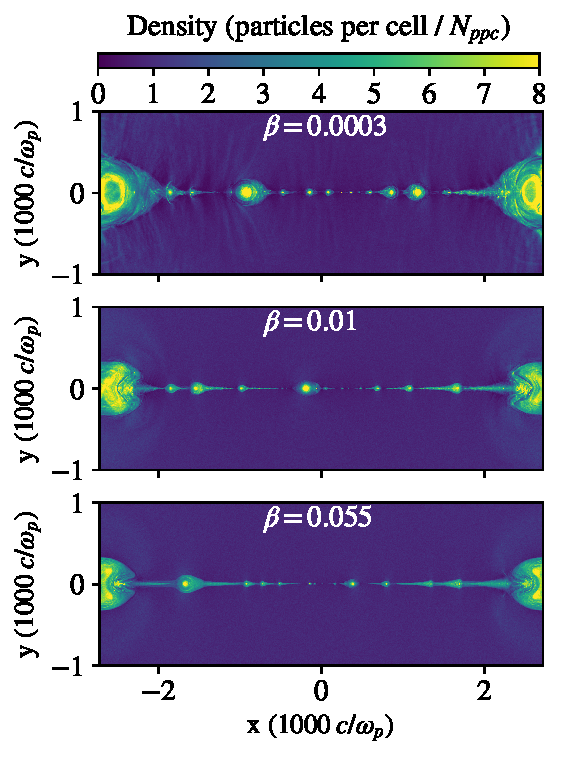
\includegraphics[width =0.5\textwidth]{sig3_threeplot.pdf}
	\caption{2D density structure  at $t\approx t_{A}$ for a suite of simulations with fixed $\sigma=3$ and varying $\beta$: $\beta=0.0003$ (top), $\beta=0.01$ (middle), and $\beta=0.055$ (bottom), corresponding to simulations D1, D4, and D6.  Secondary plasmoids form for all values of $\beta$, with larger plasmoids appearing in the lowest-$\beta$ simulation.}
    \label{sig3_twoplot}
\end{figure}


%%%%%%%%%%%%
\section{The Role of $\beta$ in the Dynamics of the Reconnection Layer}\label{role_of_beta}
In this Section, we illustrate how the dynamics in the reconnection layer depends on plasma beta and magnetization. At first, we study the role of $\beta$ in the  development of 2D structures  in the reconnection region (e.g., secondary plasmoids and X-points), and then we investigate the dependence on $\sigma$ and $\beta$ of the inflow rate (or equivalently, of the rate of magnetic field dissipation). In the next Section, we will study the dependence on $\sigma$ and $\beta$ of the particle energy spectrum.

We show in Figure \ref{sig_3_twoplot} the 2D density structure of three simulations with fixed $\sigma=0.3$ and varying $\beta$: $\beta=0.0003$ (top), $\beta=0.01$ (middle), and $\beta=0.55$ (bottom).  In Figure \ref{sig3_twoplot} we show snapshots from three simulations with $\sigma=3$ (so, one order of magnitude higher than in Figure \ref{sig_3_twoplot}) and different $\beta$: $\beta=0.0003$ (top), $\beta=0.01$ (middle), and $\beta=0.055$ (bottom). For both figures, the snapshots are taken at $t\approx t_{A}$, after the reconnection fronts have reached the boundaries of the box.

In the low-$\sigma$ case (Figure \ref{sig_3_twoplot}, for $\sigma=0.3$), we see a clear difference in the structure of the current sheet between low- and high-$\beta$ simulations (see also \citealt{rowan2017}). At low $\beta$ (top panel), the current layer is pinched by the secondary tearing mode at multiple locations along the sheet, resulting in numerous secondary X-points and plasmoids. In contrast, the highest-$\beta$ case (bottom panel), which is close to $\beta_{\rm max}\approx 1/4\sigma\simeq 0.8$, displays a smooth density profile in the reconnection outflows, with only marginal evidence for two secondary plasmoids. No prominent X-points are detected at high $\beta$ (bottom panel), with the exception of the primary X-point located at the center of the layer, resulting from our initial perturbation of the current sheet.

In the high-$\sigma$ simulations (Figure~\ref{sig3_twoplot}, for $\sigma=3$), the dependence on $\beta$ is less pronounced.  We do, however, see that the lowest-$\beta$ case (top panel) has larger plasmoids and that its current layer is broken up into distinct high-density plasmoids, separated by low-density regions.  In comparison, the highest-$\beta$ simulation in the bottom panel (with $\beta$ approaching $\beta_{\rm max}\approx 1/4\sigma\simeq 0.08$) still presents several secondary plasmoids, but the density profile in between neighboring plasmoids is smoother than at lower $\beta$. In other words, the density contrast between secondary plasmoids and X-points seems to get reduced with increasing $\beta$.

In summary, the fragmentation of the current sheet into secondary plasmoids separated by secondary X-points becomes more and more pronounced at lower $\beta$ (for fixed $\sigma$) and at higher $\sigma$ (for fixed $\beta$; compare the top and middle panels between Figure \ref{sig_3_twoplot}  and Figure~\ref{sig3_twoplot}; see also \citealt{sironi2016}, for the same conclusion in the ultra-relativistic regime $\sigma\gg1$).  It is likely that these structural differences in the appearance of the reconnection layer play a key role in whether efficient particle acceleration occurs, as we will discuss in Section \ref{mechanism}.


\subsection{Reconnection Rate}
In the whole range of $\sigma$ and $\beta$ investigated in this work, we calculate the mean inflow rate, which corresponds to the rate of magnetic field dissipation (i.e., to the so-called ``reconnection rate''). At each time, we compute the spatial average of the $y-$component of the flow velocity in a region close to the center of the domain, covering the range  $|y| \lesssim 400\; c/\omega_{p}$ and $|x| \lesssim 1000\; c/\omega_{p}$. This area is sufficiently large that it allows to obtain a proper estimate of the steady-state inflow rate, and it is chosen to exclude the boundary island, that artificially inhibits the plasma inflow rate in its vicinity. 

In Figure \ref{sigpoint3_inflow_rates}, we show the temporal evolution of the inflow rate for four representative simulations, having a fixed $\sigma=0.3$ and ranging in $\beta$ over three orders of magnitude. The inflow speed is measured in units of the upstream Alfv\'{e}n velocity $v_A$. At early times ($\omega_{p}t\lesssim 5000$), the inflow rate steadily increases, as the reconnection fronts move away from the center of the domain, and the region of inflowing plasma  extends further and further in both the $x$ and $y$ directions. 
After the reconnection rate reaches its peak, it settles around a constant value (with only a slight decrease at later times). Eventually, the boundary island would grow so large to inhibit the inflow of particles and magnetic flux, and the reconnection rate would artificially drop to zero. Figure \ref{sigpoint3_inflow_rates} suggests that, for the timespan covered by our simulations, the computational domain is sufficiently large to properly capture the steady state of reconnection, without artificial effects from the periodic boundaries.

At low $\beta$  (most notably for $\beta=10^{-4}$ and $\beta=10^{-3}$, cyan and green lines), the inflow rate displays significant fluctuations. After the peak, the reconnection rate drops. This is due to the fact that 
the first secondary plasmoids tend to form around the center of the box, and their pressure slightly inhibits the inflow of surrounding upstream plasma. Once the plasmoids get advected by the field tension towards the boundary island, the upstream plasma can freely flow into the layer, which explains the second peak in the reconnection rate (at $\omega_{p}t\sim 9500$ for $\beta=10^{-4}$ and at $\omega_{p}t\sim 13000$ for $\beta=10^{-3}$). These oscillations in the temporal profile of the inflow rate are observed for all our low-$\beta$ cases.

\begin{figure}[!h]
	\centering
{
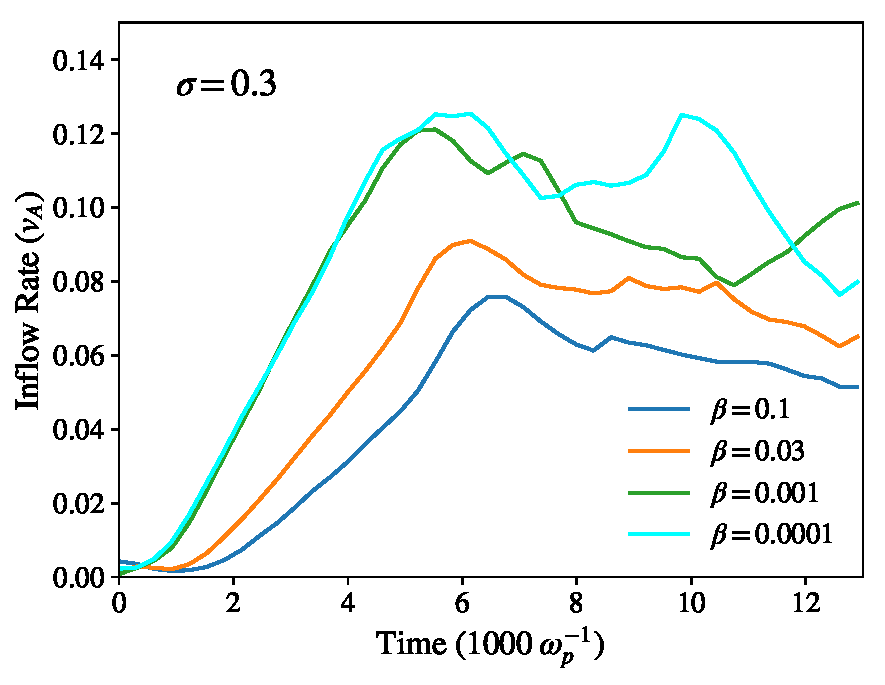
\includegraphics[width=\linewidth]{sigpoint3_inflow_rates.pdf}
\caption{\label{sigpoint3_inflow_rates}Time evolution of the inflow rate, in units of the upstream Alfv\'en speed, for four different simulations at fixed $\sigma=0.3$ and varying $\beta$ (simulations B0, B2, B6, and B7, in order of increasing $\beta$).  The inflow speed tends to decrease at higher $\beta$.}
}
\end{figure}

From  Figure \ref{sigpoint3_inflow_rates}, it is clear that the inflow rate is nearly independent of $\beta$ in the low-$\beta$ regime, but it tends to decrease at higher $\beta$. This is further confirmed by Figure~\ref{inflow_rates_over_Va}. There, we present, as a function of $\sigma$ and $\beta$, the mean reconnection rate, averaged from the peak time through a timespan of $3000 \; \omega_{p}^{-1}$ ($\sim 0.3 \,t_{A}$), when the reconnection process is  steadily active. The error bars in Figure \ref{inflow_rates_over_Va} indicate the standard deviation, which is larger at lower $\beta$, where the copious formation of secondary plasmoids causes pronounced oscillations in the inflow rates, as we have discussed above.

From Figure \ref{inflow_rates_over_Va}, we see that the inflow rate for $\beta\gtrsim 10^{-2}$ is nearly independent of $\sigma$, but it gets lower and lower for increasing $\beta$ (as already observed in MHD simulations by \citealt{ni2012}, and in PIC simulations by \citealt{rowan2017}). For $\beta\lesssim 10^{-2}$, the inflow rate is nearly $\beta$-independent (with the exception of $\sigma=3$), and tends to increase with $\sigma$ when approaching the relativistic regime $\sigma\gtrsim 1$ (see  \citealt{sironi2016} for the dependence of the inflow rate on magnetization in the ultra-relativistic regime $\sigma\gg1$). The low-$\beta$ limit at $\sigma\lesssim1$ is consistent with a fixed value of the reconnection rate, of order $\sim 0.1\,v_{A}$. 
As we further discuss in the next two Sections, the dependence of the inflow velocity on $\beta$ and $\sigma$ will be mirrored by the magnitude of the electric field in the reconnection region, which in turn impacts the rate of particle acceleration.

%In addition to the inflow rate, we have also analyzed the dependence on $\beta$ and $\sigma$ of the outflow speed. While the inflow rates are highly sensitive to $\beta$, the speed of outflowing plasma is largely independent of the plasma-$\beta$, almost always reaching of order the Alfv\'en velocity (see \citealt{rowan2017} for a detailed analysis of the $\beta$-dependence of the outflow velocity).

%\begin{figure}[b]
%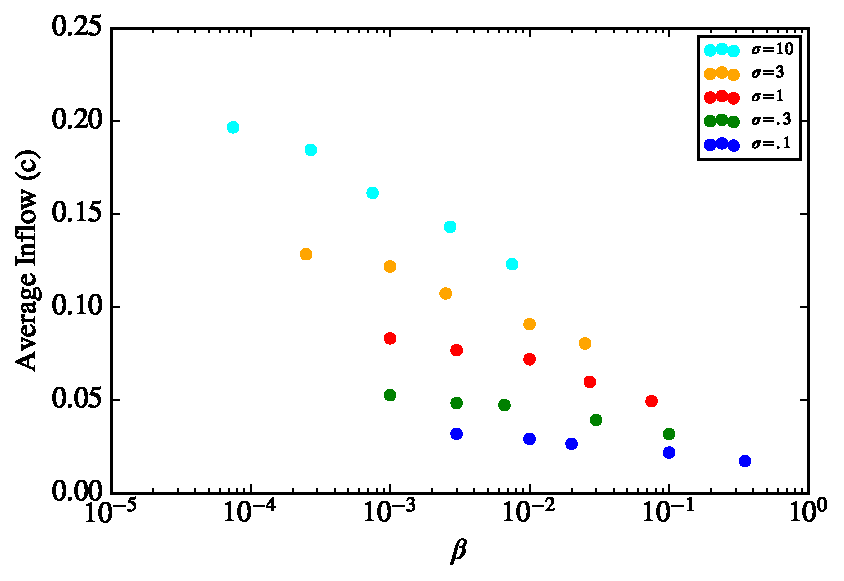
\includegraphics[width =0.5\textwidth]{inflow_rates.pdf}
%	\caption{Inflow rates across $\sigma$, $\beta$, in units of the speed of light}
%    \label{inflow_rates}
%\end{figure}


\begin{figure}[t]
	\centering
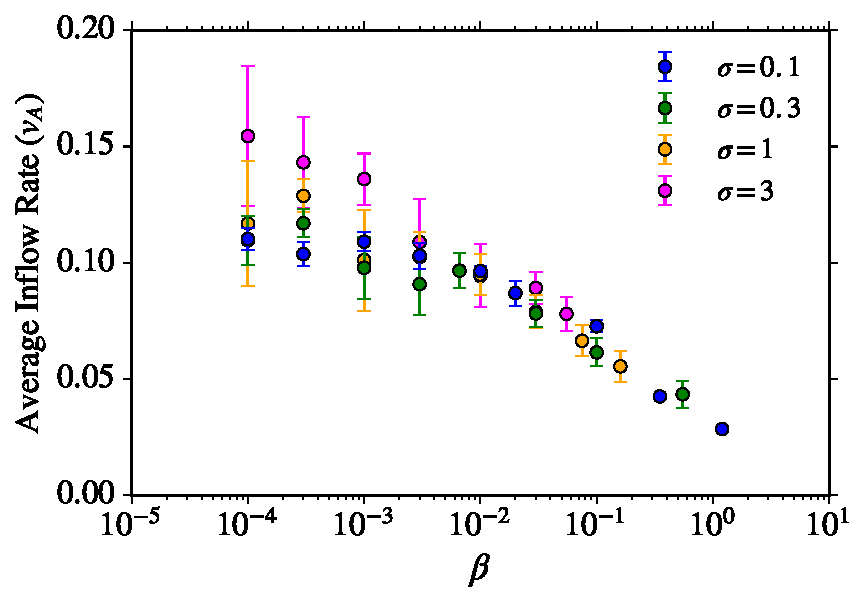
\includegraphics[width =\textwidth]{inflow_rates_over_va.pdf}
	\caption{Temporal averages of the inflow rate as a function of $\sigma$ and $\beta$, in units of the upstream Alfv\'en velocity.  The error bars indicate the standard deviation, which is larger at low $\beta$ for the copious formation of secondary plasmoids.}
    \label{inflow_rates_over_Va}
\end{figure}


\section{Dependence on  $\beta$ and $\sigma$ of the Electron Energy Spectra}\label{energy_spectra}
In this Section, we investigate the role of $\sigma$ and $\beta$ on the physics of non-thermal particle acceleration, with focus on electron acceleration. We first describe how we characterize the non-thermal electron energy spectrum in the reconnection region, finding that it can be generally modeled as a power law. We quantify how the slope of the power law and the electron acceleration efficiency depend on $\beta$ and $\sigma$. We also discuss an additional high-energy component that appears for $\beta$ approaching $\beta_{\rm max}$ in both electron and proton spectra.

%We now turn to the electron energy spectra and quantify the non-thermal component that emerges as a result of reconnection as a function of the plasma parameters.
 
\subsection{Characterizing the Electron Energy Spectra}\label{chara}
As an illustrative example of how we characterize the properties of electron spectra, we show in Figure~\ref{spec_fit_ex} the electron energy distribution for a simulation with $\sigma=0.3$ and $\beta=0.003$. The solid blue line depicts the electron spectrum measured in a slab with $|y|\lesssim 1000\,c/\omega_{p}$, as delimited by the red lines in  Figure \ref{regions}. The portion of the blue curve plotted with a thicker blue line in Figure~\ref{spec_fit_ex} indicates the energy range where the reconnection region (yellow area in  Figure \ref{regions}) contributes more than 75\%. The dashed orange line shows the Maxwellian distribution initialized in the inflow region, demonstrating that the low-energy bump in the electron spectrum is populated by particles that have yet to experience the reconnection process (and so, they should not be accounted for, when drawing conclusions on the post-reconnection particle spectrum). The high-energy component (thick blue line) is a genuine by-product of the reconnection physics. It can be modeled as a power law (compare with the dashed red line, that has a slope of $p=2.9$).

In addition to the power-law slope, we quantify the efficiency of reconnection in producing non-thermal particles, by employing the following strategy. We isolate the spectrum of the reconnection region (thick blue line), and fit its peak with a relativistic Maxwellian $f_{\rm MB} (\gamma,\theta)$ (dashed blue line in Figure~\ref{spec_fit_ex}, having a thermal spread $\theta=kT/m_e c^2\approx8$). If $\gamma_{\rm pk}$ is the peak of the electron spectrum in the reconnection region, the spectrum at $\gamma\geq \gamma_{\rm pk}$ will exceed the Maxwellian distribution (i.e., in Figure~\ref{spec_fit_ex} the thick solid blue line lies above the dashed blue line).
We then quantify 
the electron acceleration efficiency by integrating at $\gamma\geq \gamma_{\rm pk}$ the excess of the electron spectrum with respect to the best-fitting Maxwellian, normalized to the overall energy content of the spectrum. Thus, the non-thermal acceleration efficiency $\epsilon$ is defined as
\begin{equation}
\epsilon= \frac{\int_{\gamma_{\rm{pk}}}^{\infty}(\gamma-1)[ \frac{dN}{d\gamma} -f_{\rm MB}(\gamma,\theta)]d\gamma}{\int_{\gamma_{\rm pk}}^{\infty}(\gamma-1) \frac{dN}{d\gamma}d\gamma}~,
\label{efficiency_eqn}
\end{equation}
where $\theta$ is the best-fitting thermal spread. 

In Section \ref{sec:5.4}, we will employ this strategy to characterize how the non-thermal acceleration efficiency and the electron power-law slope depend on plasma beta and magnetization. We will take the electron spectrum at $t\approx 2\,t_{A}$, when the spectral shape has saturated. At this time, most of the high-energy electrons reside in the boundary island, which acts as a reservoir of particles. 

We conclude this Subsection with two remarks. First, as we discuss in Section \ref{sec:5.2}, the electron spectrum tends to soften with increasing $\beta$, so its deviations from a Maxwellian  become smaller and smaller. It follows that our determination of the electron power-law slope and non-thermal efficiency become less accurate for higher $\beta$. 

Second, as we describe in Section \ref{betamax}, a peculiarity of the extreme cases with $\beta\sim \beta_{\rm max}$ is the presence of a separate high-energy spectral component, containing a few percent of particles (the simulations where this happens are marked with an asterisk in Table 1). As we discuss below, the particles belonging to this additional component experience a different energization process than the bulk of electrons accelerated by reconnection. For this reason, we neglect this additional component when characterizing the non-thermal acceleration efficiency. In practice, for the small set of simulations with $\beta\sim \beta_{\rm max}$, we identfy the Lorentz factor where the additional component starts, and we take this as an upper limit in Equation \ref{efficiency_eqn}, rather than integrating up to infinity. 
  

\begin{figure}[!t]
	\centering
	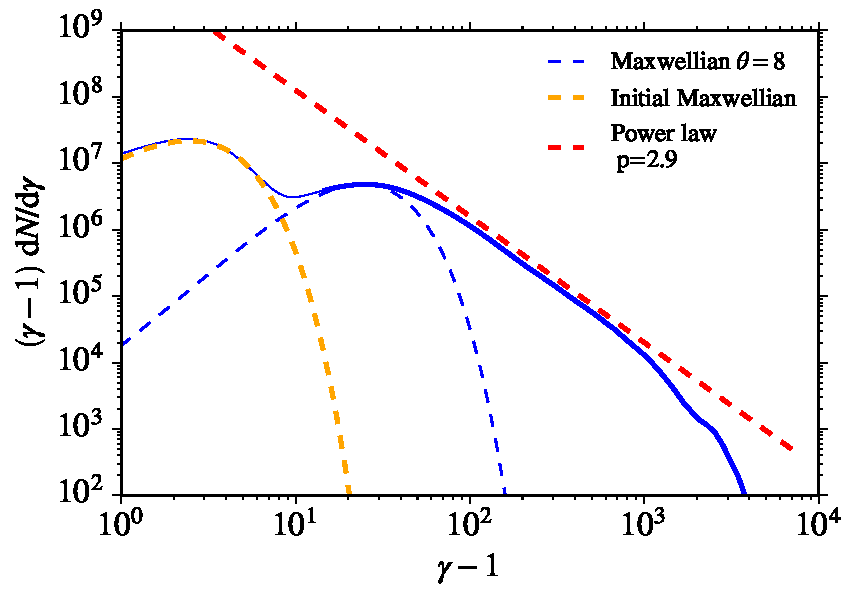
\includegraphics[width =\textwidth]{single_powerlaw_fit.pdf}
	\caption{Electron spectrum for a simulation with $\sigma=0.3$ and $\beta=0.003$ (simulation B3) taken at $t=2\,t_{A}$.  The solid blue line shows the overall spectrum in the slab delimited by the red lines in Figure~\ref{regions}, and the thick blue line marks the energy range where the spectrum is mostly contributed by the reconnection region (yellow area in Figure~\ref{regions}).  The dashed blue line shows the Maxwellian fit to the peak of the spectrum in the reconnection region, the red dashed line shows the best-fitting power law, and the orange dashed line depicts the  Maxwellian distribution initialized in the inflow region.}
\label{spec_fit_ex}
\end{figure}


\begin{figure}[!b]
	\centering
	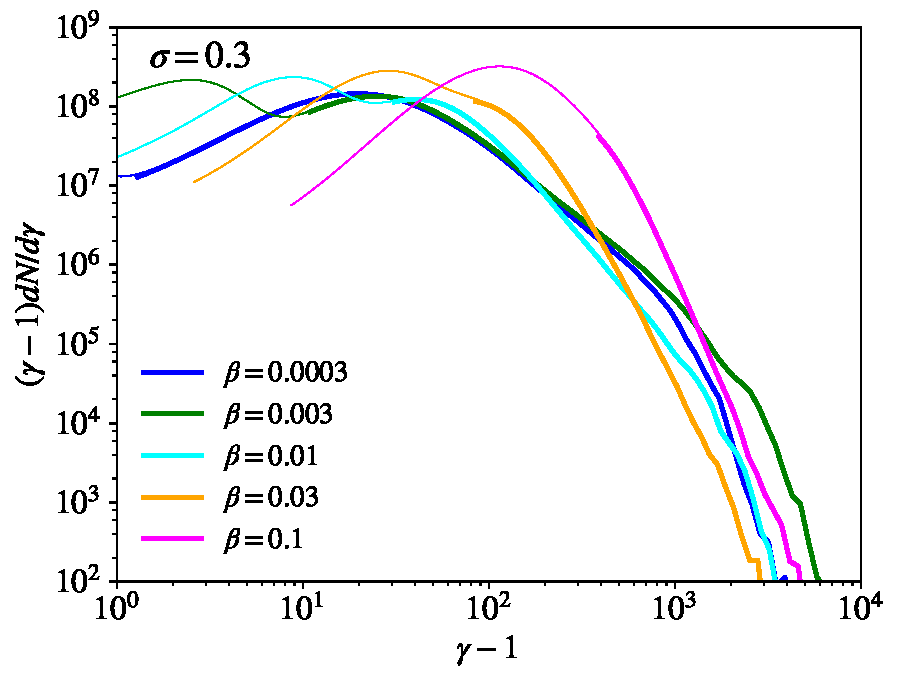
\includegraphics[width =\textwidth]{sig_3_betas_withcold.pdf}
	\caption{Electron spectra for fixed $\sigma=0.3$ and varying $\beta$, as indicated in the legend (simulations B1, B3, B5, B6, and B7), calculated at $t\approx 2\,t_{A}$.  At low $\beta$, the spectral shape converges (e.g., the blue and green curves have the same spectral slope), but as $\beta$ increases, the power law steepens significantly. Thicker lines indicate post-reconnection spectra.}
    \label{sig_3_betas_lecs}
\end{figure}

\subsection{Dependence on $\beta$  and $\sigma$ of Electron Energy Spectra}\label{sec:5.2}
In this Section, we present a few representative electron energy spectra, to illustrate the dependence on $\beta$  and $\sigma$. All  the spectra are measured at $t=2\, t_{A}$. As usual, thicker lines indicate the spectral range dominated by particles residing in the reconnection region (i.e., they display the post-reconnection spectra). 

In Figure~\ref{sig_3_betas_lecs}, we show five electron spectra from simulations with fixed $\sigma=0.3$ and a wide range of $\beta$ (see the legend). 
At low beta ($\beta\lesssim 3\times 10^{-3}$), the post-reconnection spectra (blue and green thick lines) peak at $\gamma\sim 20$, regardless of $\beta$. This is consistent with the results in \citet{rowan2017}, where it was shown that, at sufficiently low $\beta$, the reconnection process converts a fixed amount of magnetic energy into electron energy, regardless of the initial $\beta$
(so, regardless of the location of the peak in the thin lines). In addition, Figure~\ref{sig_3_betas_lecs} shows that  the shape of the post-reconnection spectrum is nearly the same for all values of $\beta\lesssim 3\times10^{-3}$. Both the power-law slope and the high-energy cutoff are insensitive to the plasma beta, in the range $\beta\lesssim 3\times 10^{-3}$. The small degree of variation in the slope and high-energy cutoff between the cases with $\beta=3\times10^{-3}$ (green) and $\beta=3\times10^{-4}$ (blue) is due to the stochastic nature of the plasmoid chain. In fact, in the $\beta=3\times10^{-3}$ simulation (green line in Figure~\ref{sig_3_betas_lecs}), a sequence of consecutive mergers leads to the formation of an unusually large secondary plasmoid. Each merger is accompanied by efficient electron acceleration (see Section \ref{mechanism}), and the peculiar merger history of the $\beta=3\times10^{-3}$ case results in the high-energy slope being slightly harder and extending to higher energies than in other simulations with comparable $\beta$ (and than in the case $\beta=3\times10^{-4}$ indicated by the blue line).

At higher beta ($\beta\gtrsim 10^{-2}$), the separation between the thermal peak of inflowing particles (thin lines) and the post-reconnection component (thick lines) shrinks, since the energy content in magnetic fields available for dissipation becomes a smaller and smaller fraction of the plasma thermal energy (compare the cyan, yellow and pink lines). In these high-$\beta$ cases, the spectrum of the plasma that has undergone reconnection can only be identified thanks to our mixing criterion, which is based on the spatial distinction between the upstream flow and the post-reconnection region (rather than on a distinction in energy space, which is impossible at high $\beta$, as Figure~\ref{sig_3_betas_lecs} shows). With increasing $\beta\gtrsim 10^{-2}$, we find that the power-law slope steadily steepens (compare green, cyan and yellow curves), and the overall spectrum  eventually resembles a single Maxwellian distribution (see the pink line). This trend holds for all the magnetizations we have investigated, as we further discuss in Section \ref{sec:5.4}.

In Figures~\ref{beta0003_spec} and \ref{beta01_spec}, we explore how the electron spectra change when varying $\sigma$, at fixed $\beta$. As $\sigma$ increases, the amount of magnetic energy available for dissipation increases, which explains the shift to higher and higher energies in the peaks of post-reconnection spectra. 
More interestingly, for $\beta=3\times10^{-4}$ (Figure~\ref{beta0003_spec}), we see that the post-reconnection spectrum becomes significantly harder with increasing $\sigma$.  The same is observed for $\beta=0.01$ (Figure~\ref{beta01_spec}), although the trend is not as prominent.

This trend --- of harder spectral slopes for higher $\sigma$ --- has been already discussed by \citet{werner2018}. In fact, the four simulations  in Figure~\ref{beta01_spec} have the same physical parameters as in \citet{werner2018}, where the dependence on $\sigma$ was investigated for the specific case of $\beta=0.01$.
In \citet{werner2018}, the electron power-law slopes for $\sigma=0.1, \; 0.3, \; 1,$ and $ 3$ were measured to be 4.0, 3.3, 2.8, and 2.4, respectively.  For these same values of $\sigma$ and $\beta$, we measure power-law indices of 4.3, 3.8, 3.6, and 3.2, i.e., we find that our spectra are systematically softer than in \citet{werner2018}. We attribute this discrepancy to the combination of two effects. First, our simulation domain for $\beta=0.01$ is about five times larger than in \citet{werner2018} (in Table 1, compare with their choice of $L_x=120\,r_{e,\rm hot}$). As we  discuss in Appendix \ref{boxsize}, larger domains systematically lead to steeper electron spectra. Second, as we describe in Appendix \ref{untriggered}, we find appreciable differences in the hardness of the electron spectrum between our setup, where reconnection is triggered in response to a large-scale perturbation, and the untriggered case, where the system evolves from particle noise. In particular, the untriggered setup generally leads to harder electron spectra. We have verified that we  recover the power-law slopes quoted by  \citet{werner2018} in the case of untriggered simulations with the same box size that they employ.


\begin{figure}[!h]
	\centering
	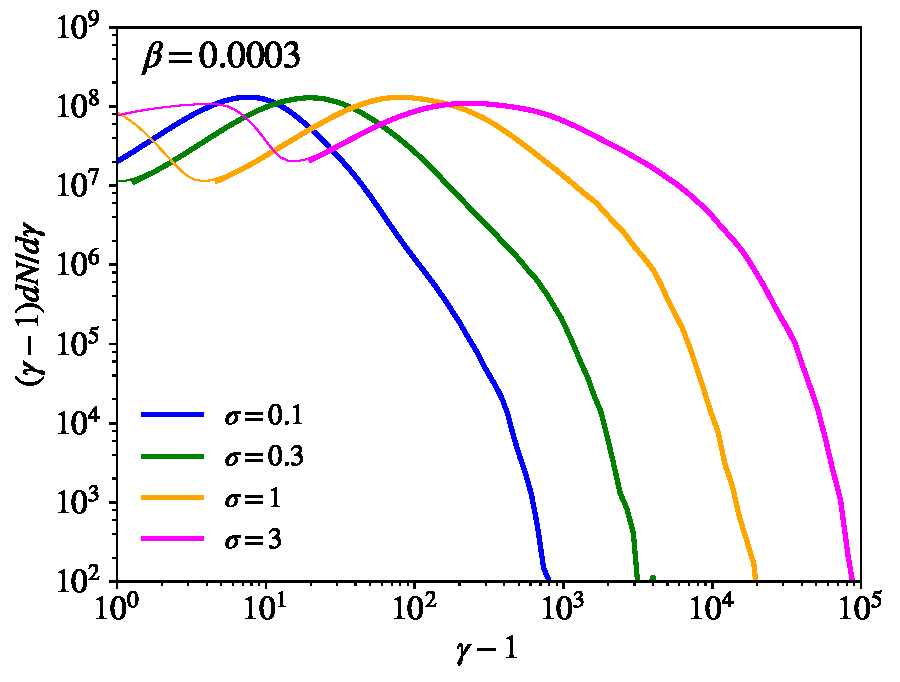
\includegraphics[width =\textwidth]{beta_0003_sigmas_withcold.pdf}
	\caption{Electron spectra for a set of simulations with fixed $\beta=3\times 10^{-4}$ and varying $\sigma$, as indicated in the legend (simulations A1, B1, C1, and D1), measured at $t\approx 2\,t_{A}$.  As $\sigma$ increases, the spectra broaden and the slope hardens.}
    \label{beta0003_spec}
\end{figure}

\begin{figure}[!h]
	\centering
	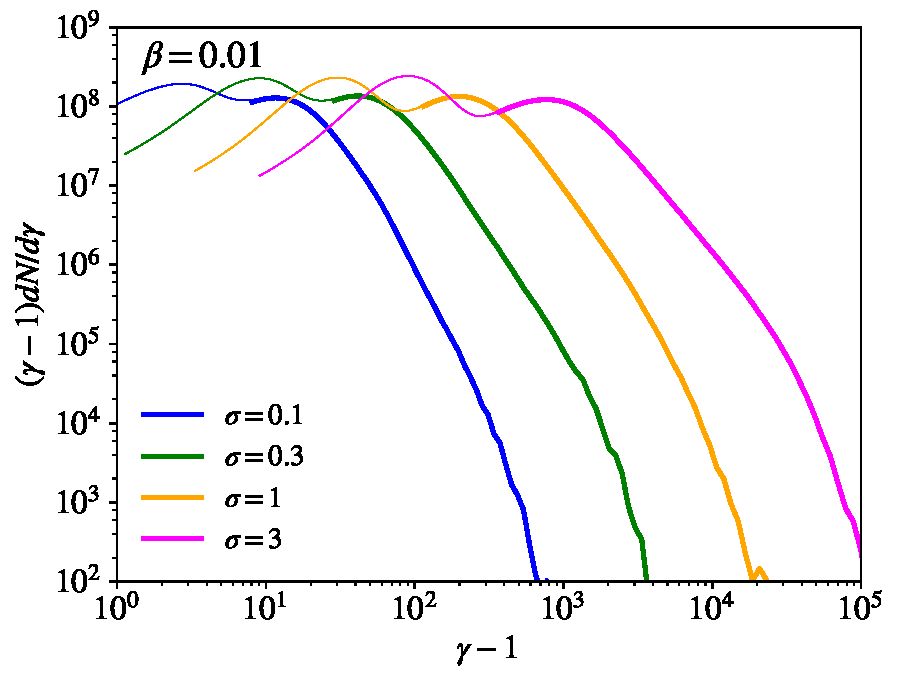
\includegraphics[width =\textwidth]{beta_01_sigmas_withcold.pdf}
	\caption{Electron spectra for a set of simulations with fixed $\beta=0.01$ and varying $\sigma$, as indicated in the legend (simulations A4, B5, C4, and D4), measured at $t\approx 2\,t_{A}$. This choice of $\beta$ is the same as in the work by  \citet{werner2018}.}
    \label{beta01_spec}
\end{figure}

\subsection{The Additional High-Energy Component at $\beta \sim \beta_{\rm max}$}\label{betamax}
A peculiarity of the extreme cases with $\beta\sim \beta_{\rm max}$ (marked with an asterisk in Table 1) is the presence of a separate high-energy spectral component emerging at late times. In Figure \ref{sig1_timespec}, we show  the temporal evolution of the electron spectrum in the simulation  that shows the strongest evidence for this additional component (i.e., the case with $\sigma=1$ and $\beta=0.16$).  

At early times ($t\lesssim t_{A}$), the high-energy part of the spectrum is very steep, barely emerging from the upstream Maxwellian (indicated by the orange dashed line). At later times ($t\gtrsim t_{A}$), an additional component appears at high energies, containing a few percent of electrons. It develops around the time when the boundary island is formed by the interaction of the two reconnection fronts across our periodic boundaries. As we show in Section \ref{mechanism}, the electrons belonging to this additional high-energy component are accelerated by bouncing between the reconnection outflow and the boundary island, in a process reminiscent of the Fermi mechanism. We remark that, as we discuss in Appendix \ref{untriggered}, this additional high-energy component is a generic outcome of high-$\beta$ reconnection. In particular, it is not an artificial by-product of our choice of a triggered reconnection setup, since it also appears in untriggered simulations. 

In Figure \ref{sig1_timespec}, we also show with a cyan line the proton spectrum at the final time (with the horizontal axis rescaled by the mass ratio, to facilitate comparison with the electron spectrum). We find that the proton spectrum displays a similar high-energy component, with just a slightly higher normalization (i.e., a slightly larger injection efficiency into the acceleration process). In other words,  electrons and protons are subject to the same  acceleration mechanism.
In retrospect, this is not surprising: in the limit that $\beta$ approaches $\beta_{\rm max}$, the upstream protons become trans-relativistic ($\theta_{i}=0.2$ for the case we show). Since the upstream electrons are also relativistic, the two species have comparable Larmor radii, and are then expected to be accelerated in a similar fashion.
 
 

\begin{figure}[!h]
\centering
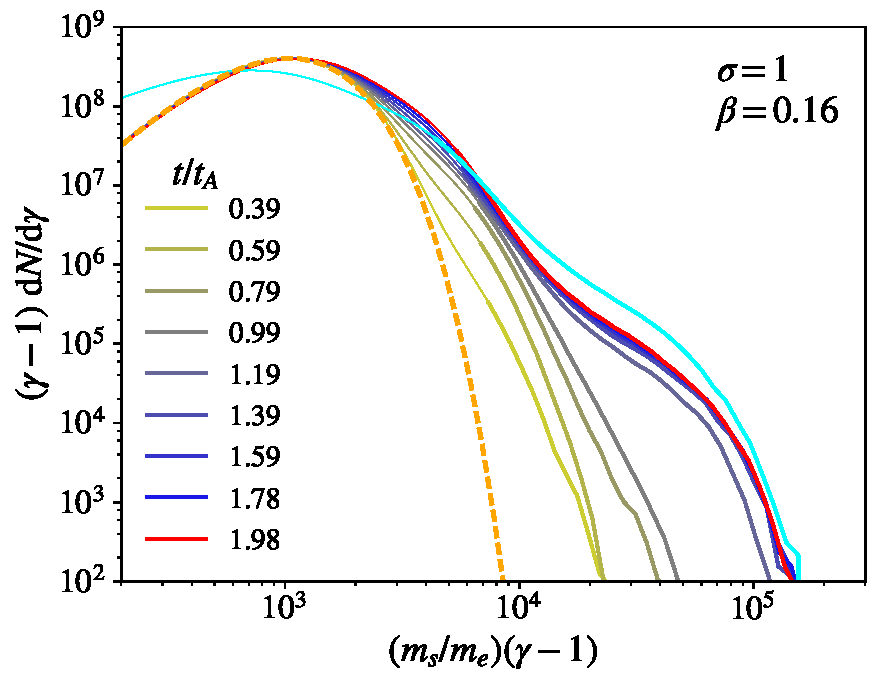
\includegraphics[width =\textwidth]{sig1_delgam_2_timespec.pdf}
\caption{Time evolution of the electron spectrum in the simulation with $\sigma=1$ and $\beta=0.16$ (simulation C7) that shows the strongest evidence for the additional high-energy component seen as $\beta\rightarrow\beta_{\rm max}$. We show the upstream electron Maxwellian with a dashed orange line. The proton spectrum at the final time is shown with the cyan line, with the horizontal axis rescaled by the mass ratio for comparison. Time is in units of the Alfv\'enic crossing time $t_A=L_x/v_A$.}
\label{sig1_timespec}
\end{figure}






%\begin{figure}[!h]
%	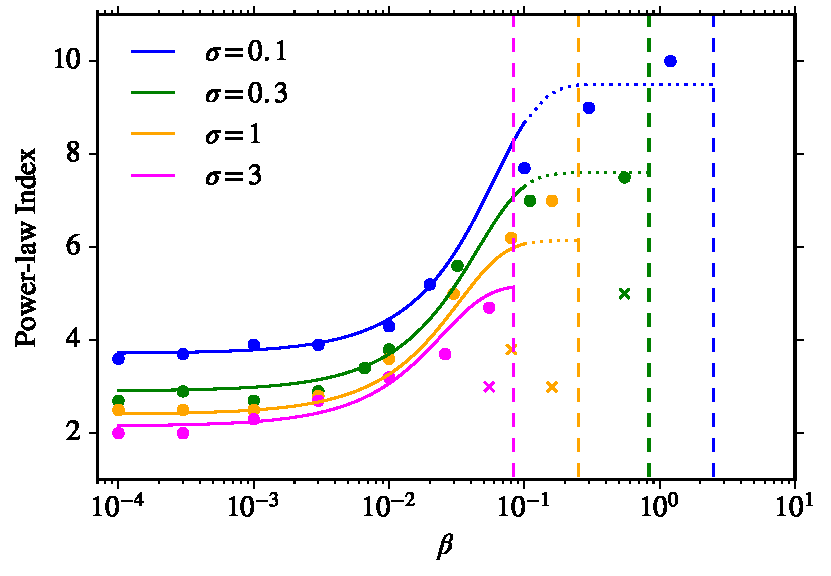
\includegraphics[width =0.5\textwidth]{powerlaw_fit.pdf}
%	\caption{Plasma-$\beta$ vs. power-law index of electron spectra.  The x's show the slopes of the hardened spectra from the secondary shock-type acceleration that occurs at high-$\beta$.}
%    \label{beta_vs_p}
%\end{figure}


%\begin{figure}[!h]
%	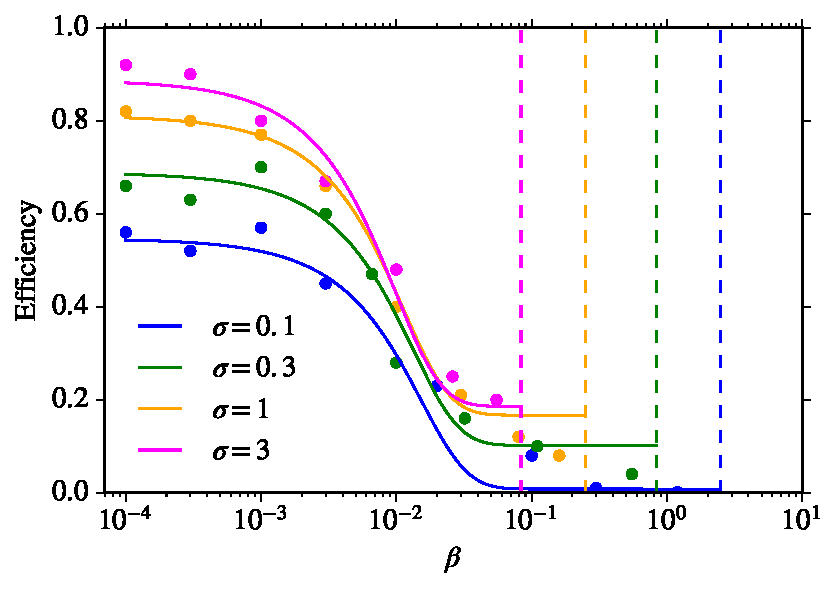
\includegraphics[width =0.5\textwidth]{efficiency_fit.pdf}
%	\caption{Plasma-$\beta$ vs. efficiency of nonthermal acceleration, defined as the ratio of nonthermal energy to total energy.}
%   \label{beta_vs_eff}
%\end{figure}

%\begin{figure}[!h]
%	\includegraphics[width =0.5\textwidth]{sig_3_betas_final_ions.png}
%	\caption{Ion spectra in the reconnection region at $\sigma=0.3$ across numerous values of $\beta$.}
%    \label{sig_3_betas_ions}
%\end{figure}



\subsection{Dependence on $\beta$  and $\sigma$ of the Power-Law Slope and Acceleration Efficiency}\label{sec:5.4}
In this Section, we summarize our results on the dependence of the electron energy spectrum on magnetization and plasma beta. In particular, in Figure \ref{powerlaw_fit} we show how the electron power-law slope depends on $\beta$ and $\sigma$, whereas in Figure  \ref{efficiency_fit} we present the dependence on $\beta$ and $\sigma$ of the efficiency of non-thermal electron acceleration, as defined in Equation \ref{efficiency_eqn}.  

In Figure \ref{powerlaw_fit}, filled circles indicate the slope of the main component of accelerated electrons, while crosses represent the slope of the additional component that emerges for $\beta\approx \beta_{\rm max}$ at late times (in the plot, the values of $\beta_{\rm max}$ for each $\sigma$ are indicated by the vertical dashed lines). When focusing on the filled circles, two trends are evident. First, at fixed $\beta$, the power-law slope is harder for higher $\sigma$ (see also \citealt{werner2018}). Second, at fixed $\sigma$ (i.e., fixed color), the slope is independent of $\beta$ for $\beta \lesssim 3 \times 10^{-3}$, but it increases (so, corresponding to a softer spectrum) at higher $\beta$, eventually resulting in a non-thermal tail that is so steep to be indistinguishable from the high-energy end of a Maxwellian distribution.

\begin{figure}[!h]
\centering
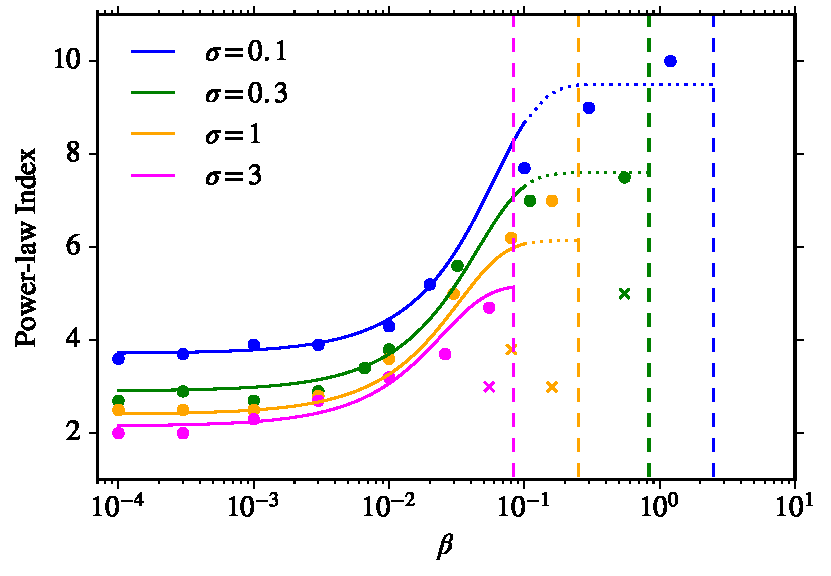
\includegraphics[width =\textwidth]{powerlaw_fit.pdf}
\caption{Electron power-law slope as a function of $\beta$ (horizontal axis) and for different values of $\sigma$ (different colors, as indicated in the legend).  The power-law indices of the main non-thermal component (i.e., the one starting from the thermal peak) are depicted with filled circles, while the power-law indices of the additional high-energy bump that appears for $\beta\sim \beta_{\rm max}$ (i.e., in the simulations marked with an asterisk in Table 1) are indicated with crosses.  The solid lines show our empirical fit in Equation \ref{initial_tanfit}. Beyond $\beta\sim 0.1$, the electron spectra become very steep and so our estimates are less robust (for this reason, our fitting curves for $\beta\gtrsim 0.1$ are plotted as dotted lines).  The values of $\beta_{\rm{max}}$ for each $\sigma$ are indicated with vertical dashed lines.}
\label{powerlaw_fit}
\end{figure}

The combined dependence of the electron slope $p$ on plasma $\beta$ and magnetization $\sigma$ can be empirically fit as 
\begin{equation}
p = A_{p} + B_{p} \tanh{(C_{p}\beta)}~~,
\label{initial_tanfit}
\end{equation}
where
\begin{equation}
\begin{aligned}
A_{p}=1.8 + 0.7/\sqrt{\sigma}~,~B_{p}=3.7\,\sigma^{-0.19}~,~C_{p}=23.4\,\sigma^{0.26}   ~.   
\end{aligned}
\label{powerlaw_fit_params}
\end{equation}
The fits are shown in Figure \ref{powerlaw_fit}  with solid lines, having the same color coding as the filled circles. For $A_p$, we have employed an expression similar to \citet{werner2018}, which properly captures the $\sigma$-dependence of our results in the limit $\beta\ll1$ (in practice, for $\beta\lesssim 3\times 10^{-3}$ we can approximate $p\simeq 1.8 + 0.7/\sqrt{\sigma}$). In particular, at $\beta\ll1$ the electron power-law slope approaches $p\simeq 1.8$ in the ultra-relativistic regime $\sigma\gg1$, whereas $p\rightarrow+\infty$ in the non-relativistic limit $\sigma\ll1$ (so, no appreciable electron acceleration in non-relativistic reconnection).

We remark that our fit is meant to capture the dependence on $\sigma$ and $\beta$ of the main component of the electron spectrum, i.e., we exclude the additional high-energy component found for $\beta\sim\beta_{\rm max}$ (so, we fit the trend in the filled circles, neglecting the crosses). Also, our fit should be employed only up to $\beta\sim 0.1$. At higher $\beta$, the electron spectra are very steep, so the power-law slope is not well constrained (as shown below, the non-thermal acceleration efficiency is negligible for $\beta\gtrsim 0.1$). For this reason, the fits above $\beta\sim0.1$ are indicated with dotted lines,  cautioning that our estimates at high $\beta$ are not very robust. 

%We find that our expression for the power-law index of a cold plasma ($\beta 3\times 10^{-3}$) is in good agreement with that presented in \citet{werner2018} (who had $\beta = 0.01$): we find $p\approx 1.8 + 0.7/\sqrt{\sigma}$, as compared to $p\approx 1.9 + 0.7/\sqrt{\sigma}$ in that study.  Note, however, that this apparent agreement is due to the fact that they use a higher plasma-$\beta$ (which softens the slope), but a much smaller box (which hardens the slope, see Appendix \ref{boxsize}).  These two effects happen to cancel eachother out for their particular choice of $\beta$. 

In addition to the power-law slope, we have also quantified the dependence on $\beta$ and $\sigma$ of the efficiency of non-thermal electron acceleration, as defined in Equation \ref{efficiency_eqn}.\footnote{As discussed in Section \ref{chara}, we remind that our calculation of the non-thermal efficiency excludes the high-energy component emerging for $\beta\sim \beta_{\rm max}$, since it results from a different energization process than the bulk of reconnection-accelerated electrons.} As shown in Figure \ref{efficiency_fit}, the dependence of the efficiency on $\sigma$ and $\beta$ mirrors the trends described above for the power-law slope. At low $\beta$ ($\beta \lesssim 3 \times 10^{-3}$), where the power-law slope is hard, the efficiency saturates at a value that is independent of $\beta$, and that is systematically larger for higher $\sigma$ (see the legend). At $\beta \gtrsim 3 \times 10^{-3}$, the electron spectrum becomes softer and softer with increasing $\beta$, eventually approaching a Maxwellian, so that the non-thermal efficiency drops to zero.

The combined dependence of the electron non-thermal efficiency $\epsilon$ on plasma $\beta$ and magnetization $\sigma$ can be empirically fit as 
\begin{equation}
\epsilon = A_{\epsilon} + B_{\epsilon} \tanh{(C_{\epsilon}\beta)}~,
\label{fiteff}
\end{equation}
where
\begin{equation}
\begin{aligned}
A_{\epsilon}=1 - \frac{1}{4.2 \sigma^{0.55}+1}~,~B_{\epsilon}=0.57\,\sigma^{0.18}~,~C_{\epsilon}=-87\,\sigma^{0.26}   ~.   
\end{aligned}
\end{equation}
The fits are shown in Figure \ref{efficiency_fit}  with solid lines, having the same color coding as the filled circles. In our empirical fit, the efficiency tends to zero for $\sigma\ll1$ (i.e., in the limit of non-relativistic reconnection) and towards 1 for $\sigma\gg 1$ (in the limit of ultra-relativistic reconnection).


\begin{figure}[!h]
\centering
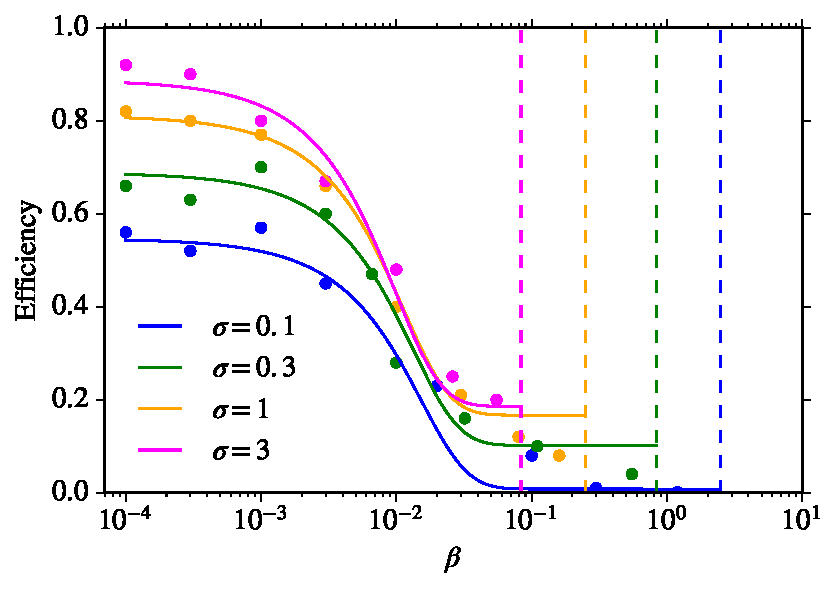
\includegraphics[width =\textwidth]{efficiency_fit.pdf}
\caption{Electron non-thermal acceleration efficiency $\epsilon$ as a function of $\beta$ (horizontal axis) and for different values of $\sigma$ (different colors, as indicated in the legend). The solid lines show our empirical fit in Equation \ref{fiteff}. For each $\sigma$, the solid lines extend up to maximum allowed $\beta$, i.e., $\beta_{\rm max}=1/4\sigma$.}
\label{efficiency_fit}
\end{figure}



\section{Electron Acceleration Mechanisms}\label{mechanism}
In order to understand the dependence on $\beta$  of the electron spectrum as discussed in the previous Section, it is instructive to investigate the physics of electron acceleration in our simulations.  To this end, we follow individual trajectories of the highest energy electrons in order to identify where they gain most of their energy and what are the physical processes responsible for their acceleration. We focus here on a few representative high-energy electrons. In a forthcoming paper, we will explore the physics of electron acceleration in greater detail.

We show in Figures \ref{lowbeta_prtl} and \ref{highbeta_prtl} the trajectories of two representative electrons. The former refers to a low-$\beta$ case with $\beta=3\times 10^{-4}$ and $\sigma=0.3$ (here, the high-energy electron belongs to the main component of particles accelerated by reconnection), while the latter refers to a high-$\beta$ case with $\beta=0.16\approx \beta_{\rm max}$ and $\sigma=1$ (here, the high-energy electron belongs to the additional component appearing when $\beta\approx \beta_{\rm max}$).

In Figures \ref{lowbeta_prtl} and \ref{highbeta_prtl}, the vertical axis represents time, in units of the Alfv\'en crossing time $t_A$. The background color in panel (a) shows the space-time diagram of  particle density. At each time, a 1D slice of density is extracted at $y=0$ (i.e., along the plane of the current sheet), and plotted as a function of $x$ (horizontal axis). The temporal evolution of the particle $x$-location is overplotted with a sequence of points, whose color corresponds to its energy (from cyan at the initial time, to pink at the final time). In panel (b), the orange line presents the time evolution of the particle $y$-position. Its first interaction with the current sheet (i.e., at $y=0$) is marked with the dashed horizontal line. Note that the $x$-position of the particle depicted in panel (a) can be meaningfully compared with the background density only when the particle $y$-coordinate in panel (b) is small (i.e., the particle is in the vicinity of the plane $y=0$ of the reconnection layer, where the density slices in panel (a) are taken).
In panel (c), we show the electron Lorentz factor $\gamma$. 
 In panel (d), we plot the temporal evolution of the quantity $E_{z}/\beta_{A}B_{xy}$ measured at the particle location, i.e., the out-of-plane electric field $E_z$ divided by the product of the in-plane magnetic field $B_{xy}=(B_{x}^{2}+B_{y}^{2})^{1/2}$ and the dimensionless Alfv\'en velocity $\beta_A=\sqrt{\sigma/(1+\sigma)}$. This will prove to be a useful diagnostic of the particle acceleration mechanisms, for the following reason: reconnection outflows move at roughly the Alfv\'en speed, so the motional electric fields carried by a magnetic field $B_{xy}$ are expected to be $E_{z,\rm ideal}\sim \beta_{A}B_{xy}$, in ideal MHD. On the other hand, in regions of strong magnetic dissipation  (e.g., at  X-points), non-ideal electric fields can largely exceed the MHD expectation, i.e., $E_z\gg E_{z,\rm ideal}$. It follows that when the ratio $E_{z}/\beta_{A}B_{xy}$ exceeds unity, it is likely that the particle is experiencing a strong non-ideal electric field, which can serve as an efficient particle accelerator.
   

\begin{figure*}[!t]
\centering
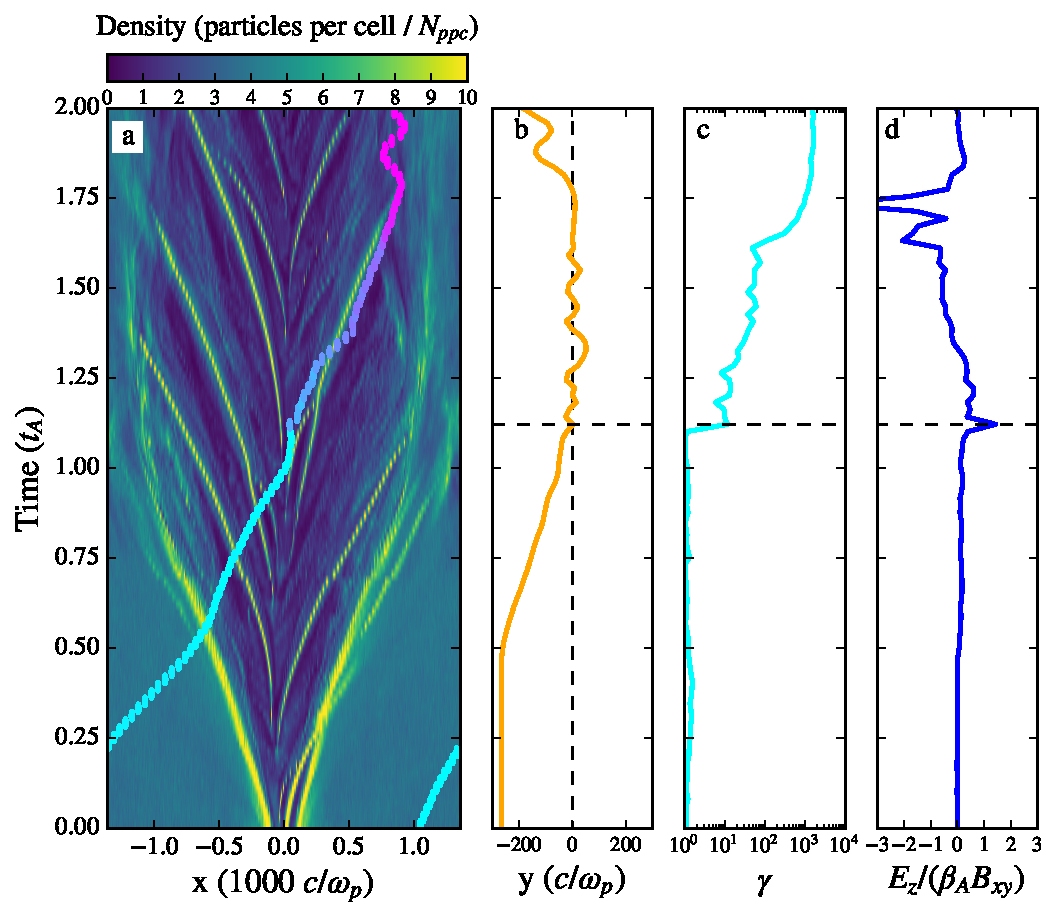
\includegraphics[width =\textwidth]{lowbeta_lec.pdf}
\caption{Representative electron trajectory from a simulation with $\sigma=0.3$ and $\beta=3\times 10^{-4}$ (simulation B1), whose temporal evolution of particle density and energy spectra is presented in  Figures \ref{lowbeta_threeplot} and \ref{timespec}, respectively. The vertical axis represents time in units of the Alfv\'en crossing time $t_A$.
The background color in panel (a) shows the space-time diagram of  particle density, composed of a sequence of 1D slices taken at $y=0$ (i.e., along the plane of the current sheet). The temporal evolution of the particle $x$-location is overplotted with points, whose color corresponds to the electron energy (from cyan at the initial time, to pink at the final time). In panel (b), the orange line presents the time evolution of the particle $y$-position. Its first interaction with the current sheet is marked with the dashed horizontal line. In panel (c), we show the electron Lorentz factor $\gamma$.  In panel (d), we plot the temporal evolution of the quantity $E_{z}/\beta_{A}B_{xy}$ measured at the particle location, which proves to be a useful diagnostic of the particle acceleration mechanisms. We find that the electron (and in general, all the high-energy electrons in low-$\beta$ runs) is accelerated by non-ideal electric fields at X-points, either in the main layer, or in current sheets formed during plasmoid mergers.}
\label{lowbeta_prtl}
\end{figure*}

%%%%%%%%%%%%%
\subsection{Electron Acceleration at Low $\beta$}
We show in Figure \ref{lowbeta_prtl} a representative high-energy electron extracted from a simulation with $\sigma=0.3$ and $\beta=3\times 10^{-4}$. For this case, we have presented the temporal evolution of the particle density in Figure \ref{lowbeta_threeplot} and of the electron and proton energy spectra in Figure \ref{timespec}.

A comparison of panel (b) and (c) demonstrates that the electron is first accelerated when it interacts with the current sheet for the first time (i.e., at the time marked by the horizontal dashed line). During this first interaction with the layer, the particle experiences a value of $E_{z}/\beta_{A}B_{xy}$ larger than unity (panel (d)), indicating that acceleration is driven by non-ideal electric fields. In fact, panel (a) shows that during this acceleration episode the electron is located in one of the under-dense regions associated with X-points. Accelerated by the non-ideal electric field, the electron Lorentz factor at the X-point quickly increases from $\gamma\approx 1$ up to $\gamma \approx 20$ (panel (c)).

The electron is then trapped in a secondary plasmoid, which can be identified in panel (a) as the yellow structure that the particle orbit follows at $1.2\lesssim t/ t_A\lesssim 1.7$. While in the plasmoid, the electron energy stays nearly constant, aside from a moderate increase (by roughly a factor of two) when the electron moves from the trailing to the leading edge of the plasmoid at $t\simeq 1.3\, t_A$. 

At $t\simeq 1.7\, t_A$, when the plasmoid merges with the boundary island, the electron lies in between the two. At the interface of the two  merging structures, a current sheet forms along the $y$ direction, i.e., perpendicular to the main reconnection layer (e.g., see the interface at $x\approx -1500 \, c/\omega_{p}$ in Figure \ref{lowbeta_threeplot}(c)). As it happens for the main layer, the newly developed current sheet breaks into a series of secondary plasmoids separated by X-points. At one of such X-points, the non-ideal electric field further increases the electron energy up to  $\gamma \approx 10^3$. The role of the non-ideal electric field is revealed in panel (d) by the peak with $E_{z}/\beta_{A}B_{xy}\lesssim -2$ at $t\simeq 1.7\, t_A$. Its sign is consistent with the fact that the non-ideal electric field in between merging plasmoids is expected to have opposite direction than in the main layer (i.e., it is oriented along $-\bm{\hat{z}}$ rather than $+\bm{\hat{z}}$). 

While many low-$\beta$ electron trajectories resemble the one we have presented here, some electrons show only one episode of acceleration, analogous to either the first or the second stage shown in Figure \ref{lowbeta_prtl}. In other words, 
some electrons pick up all of their energy at an X-point during their first interaction with the current sheet (either at the primary X-point or at one of the secondary X-points), while others are accelerated at current sheets formed when secondary plasmoids merge with each other or with the boundary island.  In either case, in low-$\beta$ simulations all the high-energy electrons are predominantly accelerated by non-ideal electric fields associated with reconnecting magnetic fields, either at the primary X-point, at secondary X-points, or in current sheets formed during plasmoid mergers.


\begin{figure*}[!t]
\centering
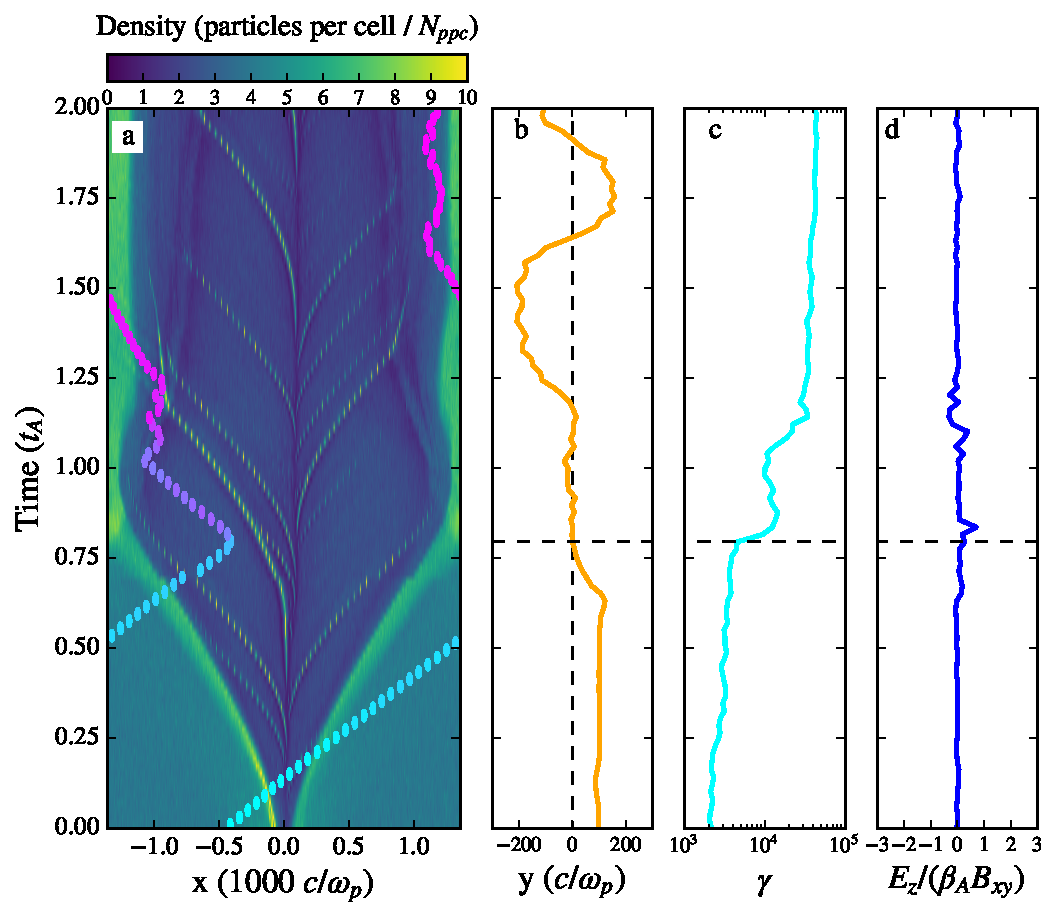
\includegraphics[width =\textwidth]{highbeta_lec.pdf}
\caption{Electron trajectory from a simulation with $\sigma=1$ and $\beta=0.16$ (simulation C7), as a representative case of particles (both electrons and protons) belonging to the additional high-energy component appearing for $\beta\approx \beta_{\rm max}$. The temporal evolution of the corresponding electron energy spectrum is shown in Figure \ref{sig1_timespec}. See Figure \ref{lowbeta_prtl} for a description of the content of the panels.  We find that most of the particle energy gain comes from a Fermi-like process, while the electron is bouncing between the reconnection outflow and the edge of the boundary island.}
\label{highbeta_prtl}
\end{figure*}


\subsection{Electron Acceleration at $\beta\approx \beta_{\rm max}$}
We show in Figure \ref{highbeta_prtl} the trajectory of a representative electron from a simulation with $\sigma=1$ and $\beta=0.16$. This is the simulation that shows the strongest signature of the additional high-energy component appearing at late times for $\beta\approx \beta_{\rm max}$. The temporal evolution of the corresponding electron spectrum is shown in Figure \ref{sig1_timespec}.

Two phases of energization are seen in the time evolution of the electron energy (panel (c)). The first one (with an increase in Lorentz factor from $\gamma \approx 2\times 10^3$ up to $\gamma \approx 10^4$) is associated with the first encounter with the current sheet (as marked by the horizontal dashed line), in a similar way as we have discussed above for the low-$\beta$ case. However, the electron in  Figure \ref{highbeta_prtl} interacts with the unstructured outflow, and not with an X-point (see panel (a)). As a result, the value of $|E_{z}|/\beta_{A}B_{xy}$ along the electron trajectory (panel (d)) is much smaller than in the low-$\beta$ case. Most of the inflowing electrons experience this acceleration episode at their first encounter with the current sheet, regardless of where they interact. So, unlike in the low-$\beta$ case, they do not need to enter the layer at an X-point in order to be accelerated. Since such an energization phase is common to the majority of electrons, it should be regarded as bulk heating, rather  than non-thermal particle acceleration. In fact, an electron with $\gamma \approx 10^4$ (as appropriate for the electron in Figure \ref{highbeta_prtl}, after the first energization episode) would not belong to the high-energy spectral component seen in Figure \ref{sig1_timespec} (that lies at $\gamma\gtrsim 2\times 10^4$). 

After it reaches the outskirts of the boundary island at $t\simeq t_A$, the electron is  accelerated up to $\gamma \approx 7\times 10^4$ (so, well within the energy range covered by the high-energy component in Figure \ref{sig1_timespec}).  From $t\simeq t_A$ to $t\simeq1.2\, t_A$, it stays confined between the boundary island and the reconnection outflow. We attribute the energy increase in this phase (panel (c)) to a Fermi-type process in between converging flows (i.e., the reconnection outflow and the boundary island), for two main reasons: (\textit{i}) as in the first phase of energization, this second episode does not arise from a strong non-ideal electric field (panel (d)), as it would rather be expected for X-point acceleration; (\textit{ii}) the fractional energy gain is comparable between the first and second phases of energization, as expected for a Fermi-like process (see the next Subsection).

We find that all of the highest energy electrons in $\beta\approx \beta_{\rm max}$ simulations show this Fermi-type acceleration as they get trapped between the reconnection outflow and the boundary island. Also,  the highest energy protons in  $\beta\approx \beta_{\rm max}$ simulations display the same acceleration physics as electrons, which explains the similarity between the energy spectra of the two species (compare red and cyan lines in Figure \ref{sig1_timespec}).

%The dominant acceleration mechanisms present in this high-$\beta$ simulation seems to be more similar to shock acceleration, where particles are sampling convergent velocity fields across overdense regions (the outflow and boundary island), rather than x-point acceleration, where electrons are accelerated by non-ideal electric fields in underdense environments (x-points).

%In order for particles to sample the velocity difference between the outflow and the island, they must have Larmor radii that are on the same scale as the velocity convergence, which will be on proton scales (i.e., $\sim$ 1 proton skin depth).  The Larmor radius of an electron in units of the proton skin depth is
%\begin{equation}
%\frac{\rho_{e}}{d_{i}} = \gamma_{e}\frac{v_{e}}{c}\frac{m_{e}}{m_{i}}\frac{1}{\sqrt{\sigma_{i}}}.
%\end{equation}
%Considering the high-$\beta$ electron we show in Figure \ref{highbeta_prtl}, we see that after the electron's first interaction with the current sheet, it has a Lorentz factor of roughly $10^{4}$.  At this point, the electron's Larmor radius is $\approx$ 3.5, large enough for the electron to sample velocity convergence between the outflow and the boundary island, and receive another boost in energy, up to its final value of $\gamma \approx 10^{5}$.



\subsection{Comparing the Acceleration Mechanisms}
In this Subsection, we present a few qualitative arguments to justify why X-point acceleration plays a more significant role at low $\beta$, whereas the Fermi process is predominant at high $\beta$ (and more specifically, at $\beta\approx \beta_{\rm max}$). We defer a more detailed analysis of the physics of particle acceleration to a future study.

First, as shown in Figures \ref{sig_3_twoplot} and \ref{sig3_twoplot}, low-$\beta$ simulations display a much higher number of secondary plasmoids (and consequently, of secondary X-points) than high-$\beta$ runs. It follows that the fraction of inflowing electrons that are likely to enter the current sheet at the location of an X-point --- where they can be accelerated by non-ideal electric fields --- is higher at lower $\beta$, resulting in higher acceleration efficiencies.

Second, the strength of the reconnection electric field $E_z$ is proportional to the particle inflow rate (i.e., to the reconnection rate), which steadily decreases as $\beta$ increases (at fixed $\sigma$), as shown in Figure \ref{inflow_rates_over_Va}. So, the non-ideal electric field will be weaker at higher $\beta$, resulting in a slower rate of particle acceleration at X-points.

Finally, we can compare the typical energy gains expected from one episode of X-point acceleration and one Fermi cycle, as a function of $\sigma$ and $\beta$. The electron energy gain at an X-point will equal the work performed by the non-ideal electric field, which we set to be a fraction $\sim 0.1\,\beta_{A}$ of the upstream magnetic field $B_0$. So,
\begin{equation}
\Delta\gamma_{e,\rm X} m_{e} c^{2} \approx  0.1 \beta_{A} e B_{0} L~,
\end{equation}
where $L$ is the length of the acceleration region in the $z$-direction. If $L$ is normalized to the proton skin depth, with $L=L_{di} \,c/\omega_{pi}$, we find
\begin{equation}\label{xpoint-gain-temp}
\Delta \gamma_{e,\rm X} \approx  0.1 \frac{m_{i}}{m_{e}} \frac{\sigma}{\sqrt{\sigma+1}} L_{di}~.
\end{equation}
Clearly, the energy gain for X-point acceleration is insensitive to the initial electron temperature. On the other hand, the fractional energy increase per Fermi cycle is $\sim \beta_A$, if particles bounce between the reconnection outflow (which is moving at $\sim v_A$) and the boundary island (which is stationary).\footnote{We are also implicitly assuming that the converging flows are non-relativistic, which requires $\sigma\lesssim 1$ (so that the Alfv\'en speed is non-relativistic).} It follows that
\begin{equation}\label{fermi}
\Delta \gamma_{e,\rm Fermi}\approx \beta_A \theta_e~,
\end{equation}
and if protons and electrons are set up in temperature equilibrium, 
\begin{equation}\label{fermi}
\Delta \gamma_{e,\rm Fermi}\approx \beta \frac{m_i}{m_e} \frac{\sigma^{3/2}}{\sqrt{\sigma+1}}~.
\end{equation}
% We can infer the typical values of $L_{di}$ from the typical energy gains we see in our simulations.  For the low-$\beta$ trajectory we show, the electrons are typically energized to $\gamma\approx 100$ or $1,000$ at an x-point.  This implies $L_{di}$ of around 2 to 20.
This simple argument shows that, for fixed $\sigma$, X-point acceleration will provide a larger energy gain at low $\beta$, whereas the Fermi process will be energetically dominant in the high-$\beta$ regime.



%Considering the relativistic limit of this, where Fermi acceleration will dominate over x-point acceleration, because the electrons are starting out very hot,

%\begin{equation}
%\frac{\rho_{e}}{d_{i}} \approx 3 \theta_{i} / \sqrt{\sigma}.
%\end{equation}
%Plugging in typical values of a high-$\beta$ simulation ($\sigma=1$, $\theta=0.2$), we get $\rho_{e}/d_{i} \approx 0.6$, which is about the width of the reconnection outflow.  As the temperature decreases, the electrons will become increasingly tied to the magnetic field lines and not be able to sample the large-scale velocity differences in the outflow and between plasmoids. 

%We can make an estimate for the typical $\theta$, at which Fermi reflection becomes dominant
%We can estimate the typical $\theta$, and hence, $\beta$ that the transition from x-point to Fermi acceleration is dominant,
%\begin{equation}
%\theta_{crit} = 0.1 L_{di} \sqrt{\sigma}
%\end{equation}
%in the non-relativistic case, and 
%\begin{equation}
%\Delta E / E_{0} \approx (v_{A}/c)^{2}
%\end{equation}
%in the relativistic case.  



%Additionally, if an electron interacts with an x-point, the energy gain provided by the electric field will be a smaller fraction of the initial particle energy as $\beta$ increases, while the energy gain from a Fermi-type process is directly proportional to the particle's initial energy.  This indicates that Fermi-type processes will be energetically dominant over x-point acceleration for hotter plasmas.

%Finally, we can make a simple estimate of how much energy is picked up by a particle passing through an x-point, and examine how this quantity depends on the plasma-$\beta$.  Consider a particle with a velocity in the x-y plane given by $v_{th}$.  Imagine that this particle passes through a region with constant electric field $E_{z}$, and this region has a width of $W$.  The particle's kinetic energy will change by
%\begin{equation}
%\Delta T = \int_{}^{}\vec{F} \cdot \vec{dl} =q E_{z}\Delta z.
%\label{delta_T}
%\end{equation}
%$\Delta z$ will be set by the amount of time the particle spends in the acceleration region, $t_{acc} = W/v_{th}$, and the average z-velocity.  Because we assume a constant acceleration (constant $E_{z}$ in the x-point region), we can express the average z-velocity simply as $\bar{v_{z}}= v_{z, max}/2=t_{acc} q E_{z} / (2m)$.  As such, we get $\Delta z = t_{acc}^{2} q E_{z} / 2m $.  Plugging back into Equation \ref{delta_T}, we find:

%\begin{equation}
%\Delta T = \frac{q^{2} E_{z}^{2} t_{acc}^{2}}{2m} = \frac{q^{2}E_{z}^{2} W^{2}}{2 m v_{th} ^{2}} \approx \frac{q^{2}(V_{in} B_{0})^{2} W^{2}}{2 m v_{th} ^{2}}.
%\end{equation}
%Combining our constants into a single variable, C, and substituting in for the thermal velocity, we see that
%\begin{equation}
%\Delta T = \frac{CV_{in}^{2} B_{0}^{2} W^{2}}{KT}.
%\end{equation}
%note that $B_{0}^{2} / KT$ is proportional to $\beta^{-1}$ (for fixed density, $n$).  Based off of this simple, but physically motivated picture of particle acceleration via out-of-plane electric fields at x-points, we see that the energy gain of a particle is inversely proportional to the plasma-$\beta$ due to the fact that as particles stream through the x-point at faster thermal speeds, they will spend less time being accelerated by the $E_{z}$ fields, and hence not pick up as much energy.  This dependence on plasma-$\beta$ is likely even more drastic than $\beta^{-1}$, since there is a factor of $V_{in}^{2}$, which we have seen also depends on $\beta$, with $V_{in}$ decreasing with increasing $\beta$.  


\section{Conclusions}\label{conclusions}
In this work, we have investigated with large-scale 2D PIC simulations the physics of non-thermal particle acceleration in trans-relativistic  reconnection, covering the whole parameter space in $\sigma$ and $\beta$ and employing the physical proton-to-electron mass ratio. For four values of the magnetization ($\sigma=$ 0.1, 0.3, 1, and 3), we have explored a wide range of $\beta$, from $\beta=10^{-4}$ up to the maximum possible value of $\beta$, that is $\beta_{\rm max}\approx 1/4\sigma$. 


%In addition, our computational domains are larger than previous works by at least a factor of $\sim5$.

We find that the electron spectrum in the reconnection region can be generally modeled as a non-thermal power law, but the properties of the spectrum are strongly dependent on $\beta$. At $\beta \lesssim 3 \times 10^{-3}$, electron acceleration is efficient. The electron spectrum is dominated by a hard power law, whose slope is insensitive to $\beta$ and depends on $\sigma$ as $p\simeq 1.8 +0.7/\sqrt{\sigma}$, in agreement with the result by \citet{werner2018} (that employed a fixed $\beta=0.01$). The electron power-law tail tends to steepen for larger simulation domains. By tracking a large number of particles in our simulations, we find that at low $\beta$, electrons are primarily accelerated by the non-ideal electric field at X-points, either  in the initial current layer  or in current sheets generated in between merging magnetic islands. 


At higher $\beta$, the electron power law steepens significantly, and the electron spectrum eventually approaches a Maxwellian distribution, for all values of $\sigma$ (so, the efficiency of non-thermal electron acceleration drops). At high values of $\beta$ near $\beta_{\rm max}\approx1/4\sigma$, when both electrons and protons start relativistically hot, the spectrum of both species displays an additional component at high energies, containing a few percent of particles, which are accelerated via a Fermi-like process by bouncing in between the reconnection outflow and the stationary magnetic island at the boundary of our periodic domain.

For the main population of non-thermal electrons (i.e., excluding the additional component emerging at $\beta\rightarrow \beta_{\rm max}$),
we provide an empirical prescription for the dependence of the power-law slope and the acceleration efficiency on $\beta$ and $\sigma$. We also measure the inflow rate (i.e., the reconnection rate) as a function of $\beta$ and $\sigma$, and find that, for a given $\sigma$, the reconnection rate steadily decreases with increasing $\beta$.

Our results can provide a physically-grounded prescription for non-thermal electron acceleration via magnetic reconnection, in a regime relevant to hot accretion flows like Sgr A* at our Galactic center (e.g., \citealt{ball2016}; \citealt{mao2017}; \citealt{chael2017}). When implemented as subgrid models into global MHD simulations, our findings have the potential to unveil the origin of the flaring behaviour of Sgr A* \citep{ponti17}.
% Additionally, this study expands our understanding of magnetic reconnection in a regime that is just beginning to be explored, and shows the drastic effects that changing the plasma-$\beta$ has on the outcome of reconnection.  This study serves as an important first step towards building a fully physical model of electron acceleration in the trans-relativistic regime and highlights the important role that the plasma-$\beta$ plays in the final energy spectrum.

We conclude with a few caveats. In this paper, we have only considered reconnection setups with no guide fields and equal electron and proton temperatures.  However, for application to accretion flows around black holes, we generally expect non-zero guide fields in reconnection regions (\citealt{ball2017}), and protons to be significantly hotter than electrons.  Also, we have employed 2D simulations, and one might argue that 3D effects may alter the physics of electron acceleration and the resulting electron energy spectra.
 We will explore these effects in future studies.






\section{Appendix A: Dependence on Box Size}\label{boxsize}
To test the effect of box size on our results, we perform simulations with varying box size for a number of combinations of $\sigma$ and $\beta$.  Previous studies (e.g., \citealt{werner2018}) have shown that both the power-law slope and high-energy cutoff of the electron energy spectra increase with increasing box size (i.e., at the box size increases, the spectra become steeper, but extend to higher energies).  \citet{werner2018} probed box sizes from $20-120 \; \rho_{c}$, where $\rho_{c}$ is the Larmor radius of an electron with energy $\sigma_{e}$.  The precise reason for this dependence is not yet understood.  To this end, we aim to explore how the power-law index and high-energy cutoff depend on box size in our simulations. We perform our tests for box size both at low-$\beta$, as well as in a high-$\beta$ case, which displays a second component in its spectrum.  

We show in Figure \ref{sigpoint3_boxsize} electron spectra for simulations with $\sigma=0.3$ and $\beta=0.006$, across five different box sizes, defined by the number electron skin depths along the current sheet, at values of 680, 1,360, 2,720, 5,440, and 10,880 (corresponding to 73.6, 147.2 294.5, 589, and 1,178 $\rho_{c}$).  In order to directly compare the spectra at varying box sizes, we normalize the spectra by a factor proportional to $(L_{x}^{2}$, which makes it such that there are roughly the same number of particles in the reconnection region.  We see that there is a trend of the slope increasing with increasing box size, shown in the inset of Figure \ref{sigpoint3_boxsize}.  We find that the slopes begin to level out towards our largest boxes, but note that the inset's scale is log-linear: the slope's dependence on box size is quite weak.  Additionally, we see evidence of the high-energy cutoff increasing with box size.


\begin{figure}[!h]
	\centering
	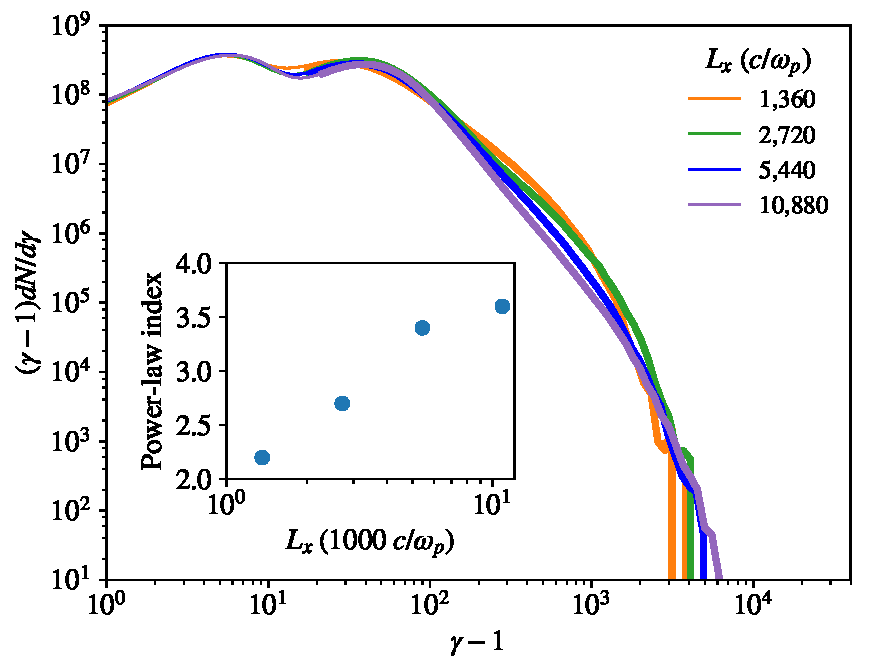
\includegraphics[width =0.75\textwidth]{sig_3_delgam001_boxsize.pdf}
	\caption{Electron spectra for $\sigma=0.3$, $\beta=0.006$, taken at $t\approx 2t_{A}$ across five different box sizes, defined by the number of cells in the direction along the current sheet (x-direction). Inset: Power-law index as a function of boxsize for the spectra shown: as the box length increases, that the power-law index gets larger.}
	\label{sigpoint3_boxsize}
\end{figure}


We also show the spectra's trend with box size for a simulation with $\sigma=1$ and $\beta=0.16$ in Figure \ref{sig1_boxsize}, a case with the extra high-energy component for our fiducial box size of 5,440 skin depths along the current sheet.  The kink in the spectra at high-energies becomes more prominent towards larger boxes: in the $L_{x}=1,360 \; c/\omega_{p}$ (orange) box, there is no notable signature of the slope hardening at high-energies. In the $L_{x}=2,720$ (green) the spectra begins to kink, and at 5,440, there's a definitive hardening in the slope just above $\gamma=10^{4}$, which persists to $\approx 10^{5}$.  Extending to even larger boxes than our fiducial case of 5,440, the feature becomes even more prominent.  We see the cutoff energy of this feature increasing (roughly linearly) with box size.  This emphasizes the importance large simulation domains in unveiling the physics of trans-relativistic magnetic reconnection.




\begin{figure}[t]
\centering
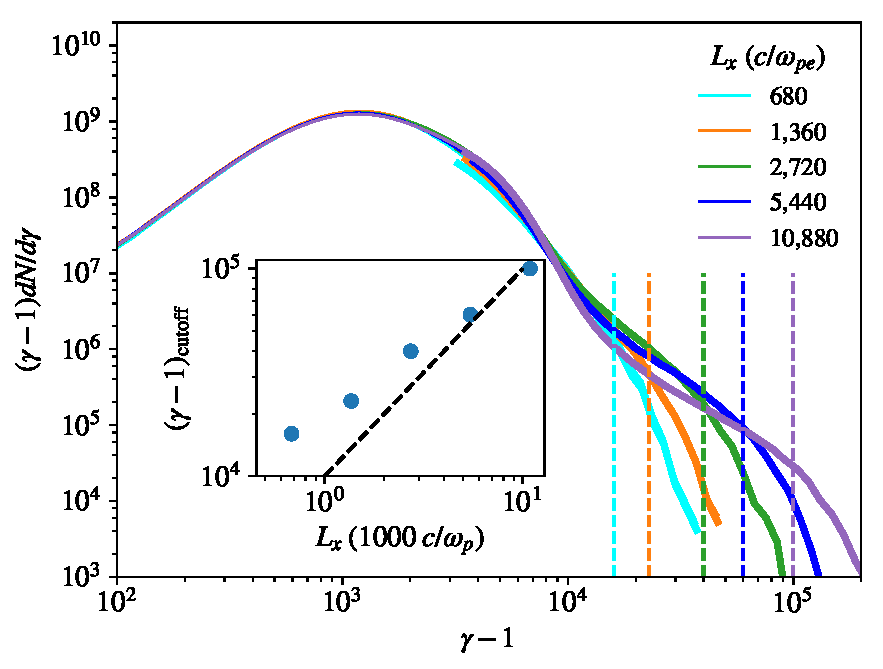
\includegraphics[width =0.75\textwidth]{sig1_delgam_2_boxsize.pdf}
\caption{Electron spectra for $\sigma=1$, $\beta=0.16$ across 5 different box sizes, taken at $t\approx 2t_{A}$.  The kink in the spectra only emerges towards larger boxes, becoming most prominent in our 16k box.  We show our estimates for the high-energy cutoff, the point at which a power-law like tail begins to exponentially fall off, with dashed horizontal lines.  The inset shows the cutoff energy as a function of box size (blue circles), while the dashed black line depicts a slope of unity for reference.}
\label{sig1_boxsize}
\end{figure}

\section{Appendix B: Boundary Conditions and Triggering Mechanisms}\label{untriggered}
In our fiducial simulations, we trigger reconnection at the center of the box and employ periodic boundary conditions in the x-direction (along the current sheet).  In this appendix, we explore the effects of these choices.  To this end, we run simulations with outflowing boundary conditions along the x-direction, as well as simulations where reconnection evolves spontaneously from noise, with no imposed triggering mechanism.  For the untriggered simulations, we employ thinner current sheets ($\Delta=20$ cells) so that the tearing instability will set in quickly.  For the outflow conditions, the setup of the current sheet is identical to the triggered simulations.

We show in Figures \ref{sigpoint3_outflow_early}-\ref{sig1_outflow_early} the spectra of three simulations at early and late times.  The spectra depicted in these figures are all from simulations with $\sigma=0.3$ and $\beta=0.006$.  The untriggered periodic, triggered periodic, and triggered outflow simulations correspond to the orange, cyan, and purple lines, respectively.  We show in the top panel of Figure \ref{sigpoint3_outflow_early}, spectra from a time before the reconnection fronts have reached the boundary in the triggered simulations.  We see at this early time that the spectra from the triggered outflow and periodic simulations are identical.  This is expected, since the outflowing plasma has not yet reached the boundaries, so the differing boundary conditions have not yet influenced the spectra.  The untriggered spectrum, however, shows a significantly harder spectrum.  In the bottom panel of the same figure, we show the spectra from the same simulations at a later time, once reconnection has halted in the periodic simulations due to finite box size and influence of the boundaries.  We see that the untriggered spectrum is still significantly harder than the triggered periodic (our fiducial choice) simulation: we measure a power-law index of 2.7 for the untriggered electron energy spectrum, while the corresponding simulation's electron energy spectra has a power-law index of 3.4.  The significantly harder electron spectrum in the untriggered case may be due to the fact that, for an untriggered simulation, the initial current layer will break up into numerous primary x-points, which may serve as sites of electron acceleration in low-$\beta$ reconnection (see, e.g., section 6.1).  In the triggered simulations, however, because we trigger the local collapse of the current sheet, there is only one primary x-point.  Additionally, in the case of untriggered reconnection, there are many more equal-sized plasmoid mergers, since the final magnetic island is assembled through the hierarchical merging of the initial plasmoids.  In contrast, in the triggered simulations, when secondary plasmoids form, they are quickly pulled towards the edge of the box, which suppresses their tendency to hierarchically merge with other plasmoids of similar sizes to build large plasmoids in the current layer, and accelerate particles during these mergers.  While these are plausible explanations for why the untriggered electron spectra are significantly harder than the triggered cases, we defer a detail physical analysis of this phenomenon to future work.  We see that the outflow simulation shows a slightly harder slope than the triggered periodic case at late times.  This may be due to some degree of thermalization that occurs when secondary plasmoids merge into the boundary island, which would then build up a larger thermal peak for periodic systems, but we defer a more thorough examination of this to future work.

\begin{figure}[!h]
	\centering
	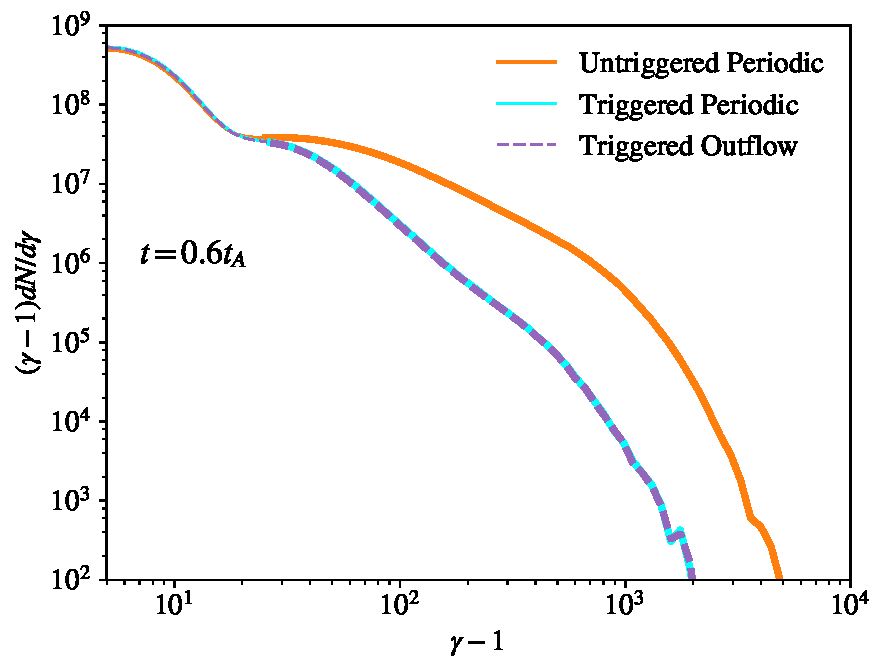
\includegraphics[width =0.75\textwidth]{sig_3_delgam001_outflow_untriggered_earlytime.pdf}
	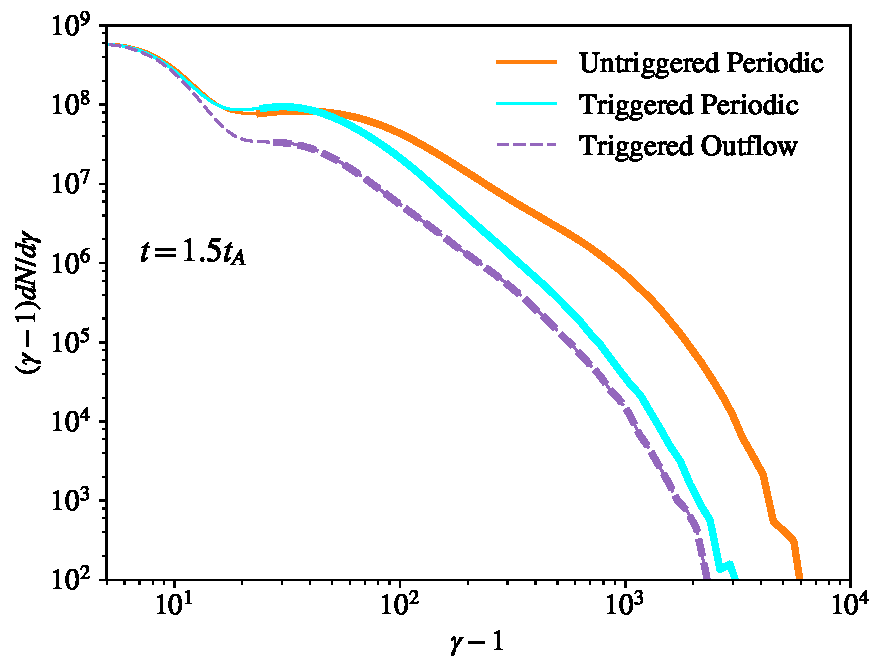
\includegraphics[width =0.75\textwidth]{sig_3_delgam001_outflow_untriggered_latetime.pdf}
	\caption{Electron spectra for simulations with $\sigma=0.3$, $\beta=0.006$ at 0.5 (top) and 2 (bottom) Alfv\'en crossing times.  The fiducial triggered and periodic simulation is shown in red.  The triggered outflow, and untriggered periodic simulations are shown in purple and orange, respectively.  In the top panel (early time), boundary effects have not yet influenced the spectra, and the two triggered simulations with periodic and outflow boundaries are identical.  The untriggered simulation, however, shows a significantly harder spectra.  At a later time (bottom), the boundaries affect the spectra and the triggered periodic simulation shows a softer slope than the triggered outflow.}
	\label{sigpoint3_outflow_early}
\end{figure}
We show plots analogous to the previous two in Figure \ref{sig1_outflow_early}, but for simulations with $\sigma=1$ and $\beta=0.16$.  We aim to see whether the extra component is due to the choice of triggering mechanisms, or it is a general feature of high-beta reconnection in large enough boxes.  We once again see that at early times (top panel of Figure \ref{sig1_outflow_early}), the triggered outflow and periodic spectra are identical, while the untriggered simulation shows a harder high-energy spectrum.  At late times (bottom panel), we see that there is a kink in the spectra of both the untriggered and triggered periodic simulations, where the spectra become harder, and extend to high energies.  While the precise characteristics of this additional component are different between the triggered and untriggered simulations, we do indeed find that it is a general feature of high-$\beta$ reconnection for large periodic systems.  In the outflow case, we do not see the signature of this feature.  This is likely due to the fact that this feature is associated with regions of strong velocity convergence, which are absent in the outflow simulations.



%\begin{figure}[!h]
%\centering
%\includegraphics[width =0.5\textwidth]{sig_3_delgam001_outflow_untriggered_spect_latetime.png}
%\caption{Electron spectra for simulations with $\sigma=0.3$, $\beta=0.006$, shown at an Alfv\'en crossing time of $\approx2$.  At this point, a significant amount of plasma has left the system in the outflowing simulation.  .The untriggered simulation shows a significantly harder spectra.}
%\label{sigpoint3_outflow_late}
%\end{figure}



\begin{figure}[!h]
\centering
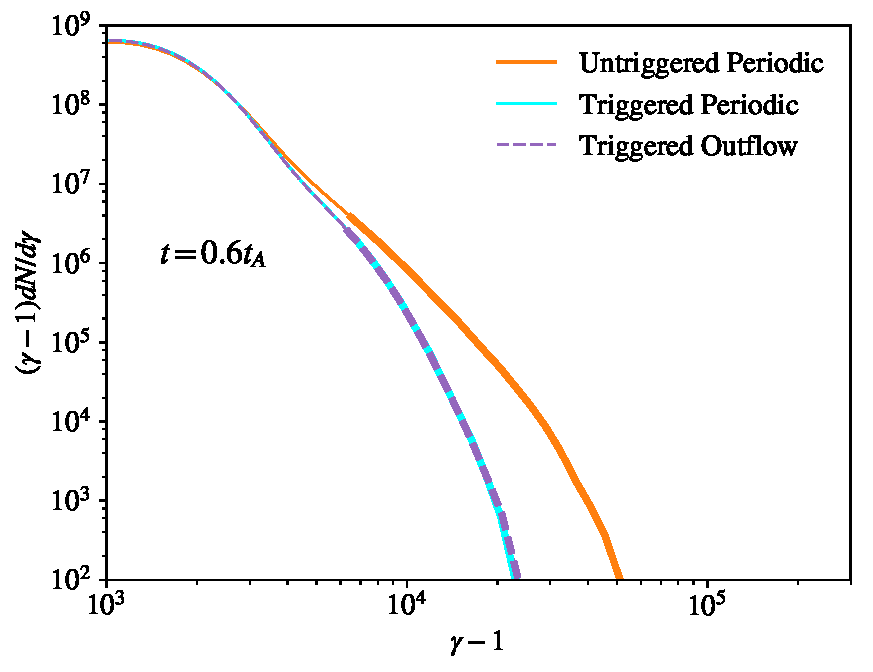
\includegraphics[width =0.75\textwidth]{sig1_delgam_2_outflow_untriggered_earlytime.pdf}
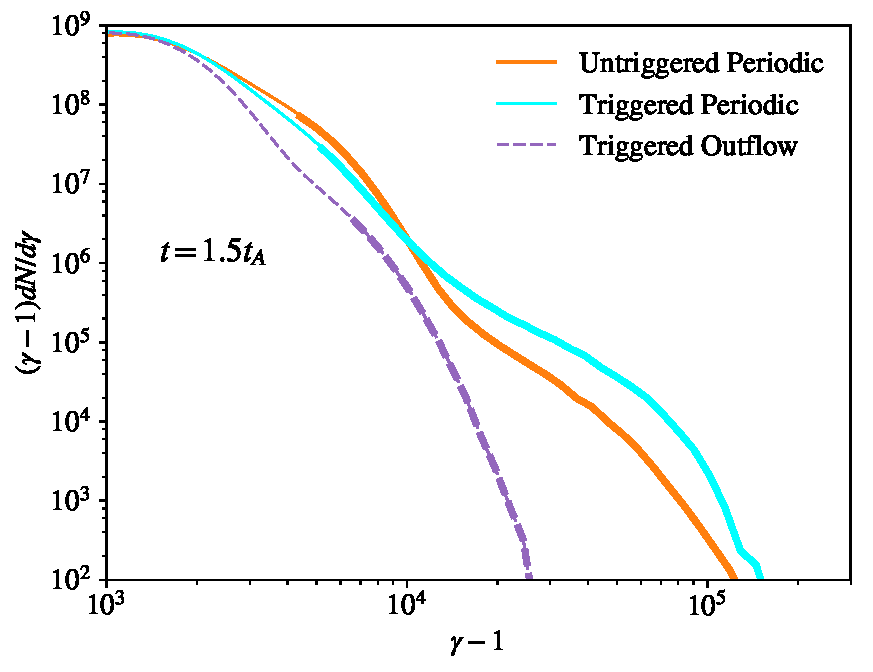
\includegraphics[width =0.75\textwidth]{sig1_delgam_2_outflow_untriggered_latetime.pdf}
\caption{Electron spectra for simulations with $\sigma=1$, $\beta=0.16$, shown at an Alfv\'en crossing time of $\approx0.5$ (top) and $approx 2$ (bottom).}
\label{sig1_outflow_early}
\end{figure}


%\begin{figure}[!h]
%\centering
%\includegraphics[width =0.5\textwidth]{sig1_delgam_2_outflow_untriggered_spect_latetime.png}
%\caption{Electron spectra for simulations with $\sigma=1$, $\beta=0.16$, shown at an Alfv\'en crossing time of $\approx2$.  We see that the high-energy kink in the spectrum emerges in both the triggered and untriggered simulations.}
%\label{sig1_outflow_late}
%\end{figure}


\section{Appendix C: Convergence tests}\label{convergence}
To ensure that our results are not being affected by our choice in the initial number of particles per cell ($N_{ppc}$) we employ, or the resolution, we perform simulations where we significantly increase these quantities.  In Figure \ref{ppc_spect}, we show the results of quadrupling the initial number of particles per cell, from our fiducial value of 4.  We find that increasing this quantity has little to no effect on the spectra.  

\begin{figure}[!h]
\centering
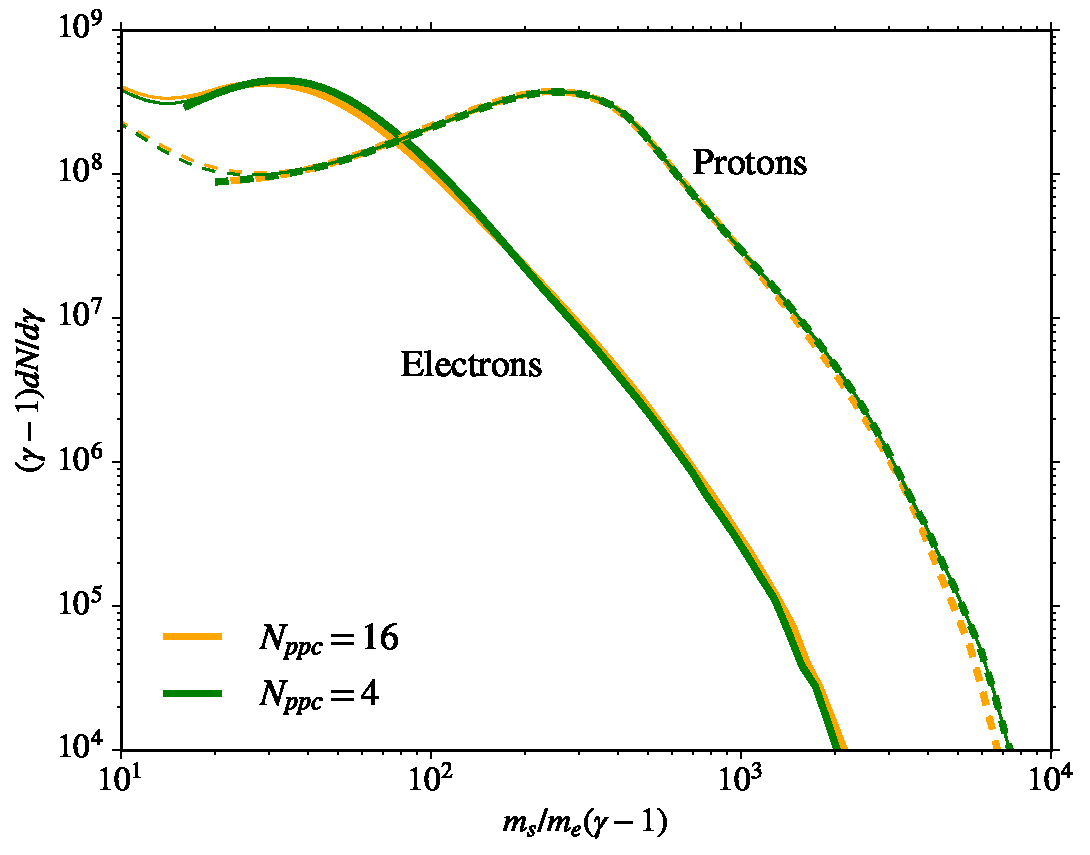
\includegraphics[width =0.75\textwidth]{ppc_final.pdf}
\caption{Electron (solid) and proton (dashed) energy spectra for simulations with $\sigma=0.3$, $\beta=0.006$, with $N_{ppc}=4$ (green) and $N_{ppc}=16$ (orange).  Spectra are computed at $t\approx 2t_{A}$  We see very little difference between the spectra from these two simulation, despite quadrupling the initial number of particles per cell.}
\label{ppc_spect}
\end{figure}

We also run a simulation where we double the spatial resolution (from our fiducial value of three cells per electron skin depth, to six), in order to ensure that our results are not sensitive to increasing the resolution.  This high-resolution simulation has the same physical box size in electron skin depths, and is compared to the fiducial run when the simulations are at equal light crossing times.  We show the electron and proton spectra in the reconnection region for these two simulations in Figure \ref{comp_spect}.  We see that the high energy slope of the electrons is unchanged, despite doubling the resolution.

\begin{figure}[!h]
\centering
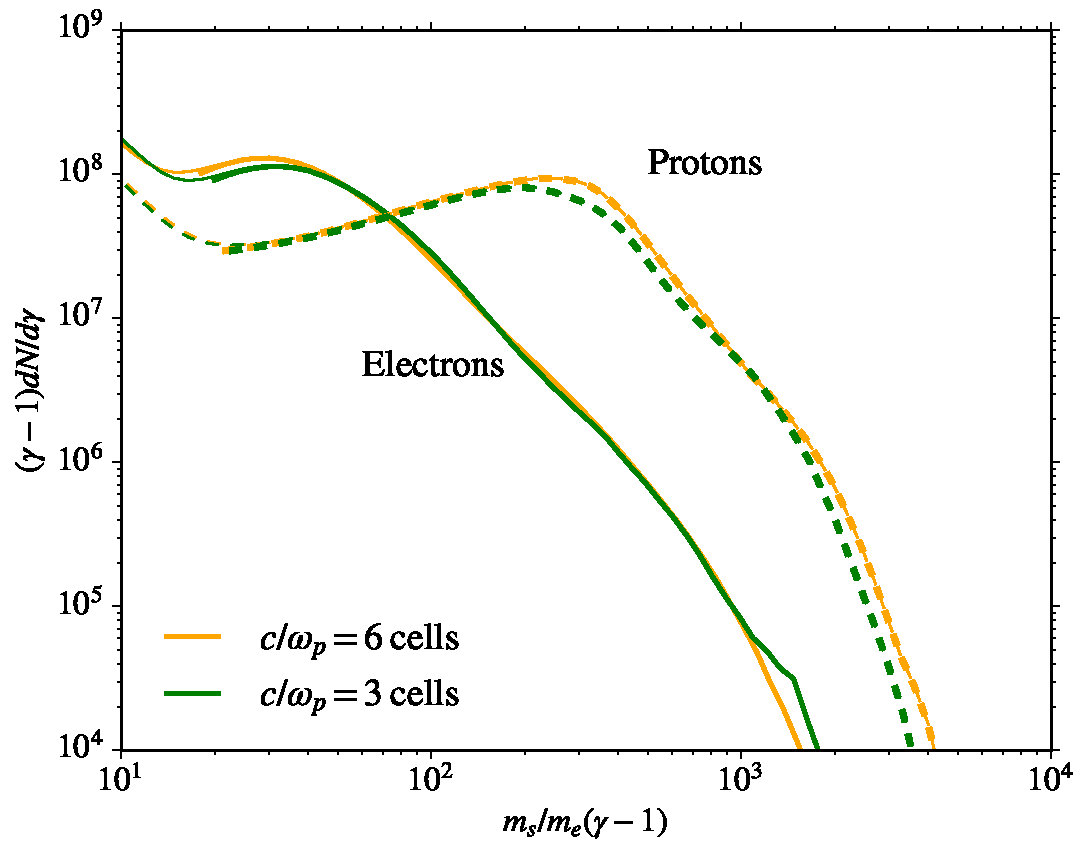
\includegraphics[width =0.75\textwidth]{comp_final.pdf}
\caption{Electron (solid) and proton (dashed) energy spectra for simulations with $\sigma=0.3$, $\beta=0.006$, where an electron skin depth is resolved in 3 (green) and 6 (orange).  Spectra are computed at $t\approx 2t_{A}$  }
\label{comp_spect}
\end{figure}


\section{Appendix D: Decomposing the Particle Spectra}\label{shells}
In order to investigate the detailed structure of the electron energy distribution and how it may change throughout the boundary island, we decompose our electron spectra into shells around the island, such as in \citet{li2017}.  Specifically, we calculate contours of the z-component of the magnetic vector potential, and break the domain into shells surrounding the largest magnetic island based on these contours.  We then extract the electron spectra from the individual shells.  We show this decomposition in Figure \ref{shellvec_spect}.  In the top panel of this figure, we show a snapshot of the density for reference.  In the middle panel, we show contours of the z-component of the magnetic vector potential, which depict the shells we will decompose the spectrum into.  In the bottom panel, we show the spectra from all the individual shells, with colors corresponding to the contours in the middle panel.  The total spectrum is shown with a solid black line.  We see that, for any given contour, the spectrum is distinctly non-thermal, with a high-energy tail that is much harder than a Maxwellian (depicted with a dashed black line, with arbitrary normalization). 

One previous study of low-$\beta$ nonrelativistic reconnection with $\sigma$ ranging from approximately 0.001 to 0.1, and $\beta$ from 0.02 to 0.2 (\citealt{li2017}) has claimed that the power-law spectrum resulting from reconnection may not be a genuine power-law, but rather the superposition of Maxwellians at varying temperatures.  We do not find this to be the case in our simulations.  This difference is likely due to the fact that their setup employed lower-$\sigma$ and higher-$\beta$ than ours.

%\begin{figure}[!h]
%\centering
%\includegraphics[width =0.5\textwidth]{shellvec_spect2.pdf}
%\caption{Electron energy spectra decomposed into shells around the large magnetic island (top).  The shells are defined by contours of the z-component of the magnetic vector potential (middle).  A spectrum of a given color in the top panel corresponds to particles from the region on the middle panel with the same color.  A Maxwellian is depicted with a dashed black line for reference.  We find that the spectra in every shell has a high energy tail that is much harder than a Maxwellian.  The bottom panel shows a snapshot of the density for reference.}
%\label{shellvec_spect}
%\end{figure}
\begin{figure}[!h]
\centering
\includegraphics[width =0.75\textwidth]{shellvec_flds.pdf}
\includegraphics[width =0.75\textwidth]{shellvec_spect.pdf}
\caption{Top: Density profile from a simulation with $\sigma=0.3$, $\beta=0.0003$ (simulation B1), taken at $t\approx 2 t_{A}$.  Middle: Contours of the z-component of the magnetic vector potential.  Bottom: electron spectra decomposed into regions based on the vector potential, colors correspond to the regions in the middle panel.  The solid black line shows the total spectrum and the dashed black line depicts a Maxwellian for reference.}
\label{shellvec_spect}
\end{figure}


\chapter[The mechanism of Electron Injection and Acceleration in Transrelativistic Reconnection]
{The mechanism of Electron Injection and Acceleration in Transrelativistic Reconnection}

\section{Introduction} \label{introduction}
The nature of reconnection depends on a few key properties of the plasma.  The ratio of magnetic energy density to enthalpy density, referred to as the ``magnetization'',
$\sigma=B_{0}^2 / 4\pi w_{0} $, where $B_{0}$ is the magnetic field strength and $w_0=(\rho_{e}+\rho_{i})c^{2}+ \hat{\gamma}_{e}u_{e}+ \hat{\gamma}_{i}u_{i}$.  Here, $\rho_{i,e}$, $\hat{\gamma}_{i,e}$, and $u_{i,e}$ are the mass densities, adiabatic indices, and internal energy densities of ambient protons and electrons, respectively.  This parameter
controls the bulk energization of the plasma.  When $\sigma$ is of order unity, we refer to the plasma as ``trans-relativistic''.  In this regime, protons remain sub-relativistic ($\gamma_{i} \approx 1$), while electrons can be accelerated to ultra-relativistic energies ($\gamma_{e} \gg 1$). 
The ratio of gas pressure to magnetic pressure, $\beta=8\pi nk_{B}T/B_{0}^{2}$ also plays an important role in the dynamics of reconnection and controls the shape of the electron energy spectrum (\citealt{ball2018}).  When $\beta$ is small, we refer to the plasma as ``magnetically dominated''.  Trans-relativistic magnetically dominated plasmas occur frequently in radiatively inefficient accretion flows such as Sgr~A* and M87*, particularly in the coronae and strongly magnetized flux tubes close the black hole's event horizon.   

Numerous PIC studies have investigated electron acceleration mechanisms in both relativistic (\citealt{sironi2014}; \citealt{nalewajko2015}; \citealt{guo2015, guo2019}; \citealt{werner2017}) and nonrelativistic reconnection (\citealt{dahlin2014,wangh2016, li_guo_2017}).  These studies generally take one of two approaches: some apply a guiding center formalism (e.g., \citealt{dahlin2014}), in which they can cleanly separate different acceleration mechanisms in the energy equation and ultimately assess the various contributions to bulk energization by looking at cell averaged currents and fields. Such a treatment will properly capture the physics of bulk heating, but will not highlight the relatively small number of accelerated particles in a high-energy non-thermal tail.  Additionally, the guiding center formalism breaks down at X-points in anti-parallel reconnection, where the magnetic field vanishes.  Others look at individual particle trajectories to assess where and by what mechanisms particles are being accelerated.  In most cases these studies sparsely sample a collection of representative particles.  Furthermore, most of these studies employ either a pair-plasma or a significantly reduced mass ratio, which may affect the conclusions. 

These previous studies have highlighted a few distinct acceleration mechanisms.  One is acceleration by the out-of-plane electric field (i.e., in the direction of the electric current) at X-points (see e.g., \citealt{zenitani2001, sironi2014, nalewajko2015}).  These X-points can occur not only in the initial current sheet via the primary or secondary tearing mode, but also in the current sheets generated between merging plasmoids.  Another prominent mechanism is Fermi reflection, enabled by the various macro-scale motions induced by reconnection which can occur within contracting plasmoids (\citealt{drake2006}) and also between outflows and plasmoids (\citealt{ball2018}).  \citet{nalewajko2015} also found that particles are accelerated in the trailing edges of accelerating plasmoids.  More recently, \citet{guo2019} found that for a relativistic pair plasma the ideal electric field and associated Fermi reflection is sufficient to produce a non-thermal distribution extending to high energies.

In \citet{ball2018} we investigated particle acceleration in the trans-relativistic regime, where the plasma magnetization (i.e., ratio of magnetic energy density to particle enthalpy density) is of order unity,  and found preliminary evidence for the role of X-points, plasmoids, and Fermi-type processes by examining the histories of a few representative high-energy electrons.  We did not, however, systematically examine an unbiased sample of electrons.  In that study, we observed that at low-$\beta$, electrons undergo extremely short periods of intense acceleration by a non-ideal electric field at X-points in the initial sheet or between merging plasmoids.  In contrast, at high-$\beta$ when electrons start out relativistically hot, X-point acceleration is negligible, and Fermi reflection dominates.  The reason for this is twofold: First, the secondary tearing mode is suppressed in thermally dominated plasmas and so the chance of interacting with an X-point is extremely low; second, the energy gain via Fermi reflection off of structures moving at the Alfv\'en speed dominates over the energy gain at X-points when the electrons already have relativistic velocities.

In this paper, we systematically investigate the physics of electron acceleration by comparing four simulations in which we vary the number of X-points and plasmoids by changing (\textit{i}) the guide field strength and (\textit{ii}) whether or not we induce reconnection by hand or let it evolve naturally via the primary tearing instability.  We use the true electron-proton mass ratio in all of our simulations to ensure that our results are not affected by using an nonphysical reduced mass ratio.  We address the issue of time downsampling by including particle acceleration diagnostics that are calculated on-the-fly during the simulation for all of the particles.  We specify the strength of the guide field as a ratio of the in-plane component and choose values of $B_{g}/B_{0}=0.1$ and $B_{g}/B_{0}=0.3$.  We choose $B_{g}/B_{0}=0.1$ because it is remarkably similar to the purely anti-parallel case in terms of the fluid structures and electron energy spectra, yet allows us to define the parallel electric field and corresponding work done by non-ideal parallel electric fields.  We choose $B_{g}/B_{0}=0.3$ as our other guide field strength because at and above this threshold, the secondary tearing mode is suppressed, simplifying the physics and allowing us to more cleanly isolate the effects of X-point acceleration.

We find that X-points formed both in the primary current sheet (PCS) as well as merger-induced current sheets (MCS) play critical roles in the first stages of electron acceleration in the trans-relativistic regime.  In particular, we find that when the secondary tearing mode is active, electron acceleration is enhanced because X-points occur more frequently throughout the current layer.  In these cases, X-points are ubiquitous, both in the PCS and MCS.  In contrast, when the secondary tearing mode is suppressed, high-energy acceleration is localized to the primary X-point(s), which are very few relative to the copious X-points that occur when secondary tearing is active.  By tracking the z-component of parallel work, we show that the first stages of electron acceleration is controlled almost entirely by this component of the non-ideal electric field associated with in-plane magnetic fields reconnecting.  After this initial acceleration, electrons are further energized through other means that may be energetically dominant to the X-point phase, but a strong correlation between $\Delta\gamma$ and the z-component of parallel work, $W_{||,z}$, remains for the high-energy electrons.  We further illustrate the importance of this pre-acceleration at X-points by including populations of test particles that only feel certain components of the parallel electric field.  We show that the z-component of parallel electric fields is critical in producing a hard non-thermal tail that extends to high energies.

The layout of the paper is as follows: in Section \ref{methods} we describe the simulations we employ, in Section \ref{diagnostics_of_acceleration} we explain the various diagnostics that we calculate on-the-fly for all of the particles in our simulation in order to understand their acceleration histories.  In Section \ref{role_of_xpoint} we show the results from our simulations and investigate the relative importance of X-points in accelerating high-energy electrons.  In Section \ref{E_comps} we investigate the role of the z-component of the parallel electric field by using our on-the-fly diagnostic of the cumulative work done on each particle by this component of the electric field.  Finally, in Section \ref{test_prtls}, we use test particles that do not feel certain components of the parallel electric field to show that parallel electric fields play crucial roles in regulating both the heating and acceleration of electrons. 

\section{Methods} \label{methods}

\subsection{Simulation Setup} \label{sim_details}
We perform four fiducial simulations of magnetic reconnection using the publicly-available code TRISTAN-MP (\citealt{buneman93}; \citealt{spitkovsky05}).  As in \citet{ball2018}, we employ a two-dimensional (2D) simulation domain in the $xy$ plane, but we track all three components of velocity and electromagnetic field vectors.  The system is periodic in the x-direction and enlarged continuously in the y-direction as the simulation progresses.  We set up the system in Harris equilibrium, with a magnetic field profile $\bm{{B}} = -B_{0}\tanh{\left(2\pi y / \Delta\right)}\bm{\hat{x}}$, where $B_{0}$ is the strength of the reconnecting field in the ambient plasma and $\Delta$ is the thickness of the sheet.  $B_{0}$ is related to the magnetization parameter $\sigma$ via $\sigma=B_{0}^2 / 4\pi w_{0} $.  We set $\sigma=0.3$ for all of our simulations.


\begin{figure*}[t]
	\includegraphics[width=\linewidth]{2x2_flds_reord.pdf}
	\caption{Snapshots of density from four fiducial simulations showing a diversity of configurations with different numbers of X-points and plasmoids.  All snapshots are taken at $t=3600 \; \omega_{p}^{-1}$, or in terms of Alfv\'en crossing times, $t_{A}=L/v_{A}$, $t \approx 0.5 t_{A}$.  The top row shows the simulations with a guide field strength of $B_{g}=0.3B_{0}$ and the bottom row shows the simulations with a guide field strength of $B_{g}=0.1B_{0}$.  The first column shows simulations where reconnection is triggered, and the second column shows simulations where reconnection develops spontaneously.
	}
	\label{lowbeta_fourdens}
\end{figure*}


\begin{deluxetable}{ccccc}
	\centering
	\tablewidth{1\columnwidth}
	\tablecaption{Simulation Parameters}  
	\tablehead{run&$B_{g}/B_{0}$& Triggered vs. Untriggered  & $L_{x}$ ($1000 \; c/\omega_{p}$) & $\Delta \; (c/\omega_{p})$ }
	\startdata
	A0& 0.3 & Triggered& 2.7 &26.66\\ 
	\hline
	A1& 0.3 & Triggered& 1.3 & 26.66\\
	\hline
	A2& 0.3 & Triggered& 5.4 & 26.66\\
	\hline
	
	B0 & 0.3&Untriggered & 2.7 & 13.33\\ 
	\hline
	B1& 0.3 & Untriggered& 1.3 & 13.33\\
	\hline
	B2& 0.3 & Untriggered& 5.4 & 13.33\\
	\hline
	B3& 0.3 & Untriggered& 5.4 & 6.66\\
	\hline
	B4& 0.3 & Untriggered& 5.4 & 20.0\\
	\hline
	C0&  0.1&Triggered& 2.7 & 26.66\\ 
	\hline
	C1& 0.1 & Triggered& 1.3 & 26.66\\
	\hline
	C2& 0.1 & Triggered& 5.4 & 26.66\\
	\hline
	
	D0&  0.1&Untriggered & 2.7 & 13.33\\ 
	\hline
	D1& 0.1 & Untriggered& 1.3 & 13.33\\
	\hline
	D2& 0.1 & Untriggered& 5.4 & 13.33\\
	\hline
	E0& 0 & Triggered& 2.7 & 26.66\\
	%\hline
	\enddata
	\tablecomments{Summary of the physical and numerical parameters of our simulations.  All simulations are performed with the physical electron-proton mass ratio, equal electron and proton temperatures, a resolution of 3 cells per electron skin depth, $\sigma=0.3$ and $\beta=0.003$.  Our four fiducial simulations are A0, B0, C0, and D0.  Simulations with the same guide field strength and triggering choice (but varying box size, current sheet width, etc.) are represented with the same letter but a different number.}
	\label{tab:fit}
\end{deluxetable}

We include an out-of-plane magnetic field (referred to as a guide field) and specify its strength as a fraction of the initial in-plane component, $B_{g}/B_{0}$.  We use two values of guide field strength, $B_{g}/B_{0}=0.1$ and $B_{g}/B_{0}=0.3$.  We specify the temperature through the proton $\beta$, defined as $\beta \equiv \beta_{i}=8 \pi n_{i} k T_{i}/B_{0}^{2}$, where $n_i=\rho_i/m_i$ is the proton number density, $T_i$ is the proton temperature, and $m_i$ is the proton mass. Ambient electrons and protons start with the same temperature, so that $\beta_e=\beta_i=\beta$ (and the total plasma-$\beta$, including both species, is $2\,\beta$).  We focus for this work on low beta reconnection, choosing a representative case with $\beta_{i}=0.003$.  At this $\beta$ and $\sigma$, the ambient protons are non-relativistic.  Because of this, the magnetization parameter as defined with the proton rest mass $\sigma_{i}=B_0^2/4\pi \rho_i c^2$ (where $\rho_i$ is the mass density of protons) is nearly identical to the enthalpy-weighted magnetization $\sigma$ defined above. 

For all of our simulations, we use the true proton-electron mass ratio, $m_{i}/m_{e}=1836$.  We initialize each computational cell in the ambient plasma with four particles per cell ($N_{ppc0}=4$).  We resolve an electron skin depth with three computational cells.   the length of our domain, along the current sheet, is 8,160 cells, corresponding to 2,720 electron skin depths.

\begin{figure*}[t]
	\includegraphics[width=\linewidth]{blines_withx.pdf}
	\caption{Snapshot of density from a triggered simulation with a guide field of $B_{g}/B_{0}=0.3$ at $t=14700 \; \omega_{p}^{-1}$ (run A0).  We superimpose streamlines of the in-plane magnetic field and emphasize two regions: the cyan box where reconnection is taking place in the initial horizontal current layer, and the red box, where reconnection is occurring between two merging plasmoids.  Note that the sign of $\vec{\nabla}\times \vec{B}$, and hence the sign of the electric field is positive in the horizontal layer (cyan box), and negative in the vertical current layer between plasmoids (red box).  We plot with red crosses the X-points identified from this snapshot.
	}
	\label{blines}
\end{figure*}

In order to achieve different numbers of X-points per unit length for simulations with identical physical parameters, we use two strategies: (\textit{i}) we let the primary tearing evolve spontaneously (hereafter, untriggered runs), (\textit{ii}) we trigger reconnection at the center of the domain.  In the former case, we use a sheet thickness of $\Delta=13.33 \; c/\omega_{p}$, where $\omega_{p}$ is the upstream electron gyrofrequency,.  In the latter case, we use a thicker sheet of $\Delta=26.66 \; c/\omega_{p}$ to ensure that no primary X-points form other than the one we induce in the center of the domain.

\subsection{Fiducial Simulations}
In order to investigate the acceleration mechanisms, our first goal is to create distinct realizations of density and field structures.  We find that one numerical and one physical parameter have the highest impact on the structure of the current sheet and can give us a great diversity of current layers.  The numerical parameter is whether or not trigger reconnection is triggered, which affects the number of primary X-points and plasmoid mergers, while the physical parameter is the strength of the guide field. 

 All PIC studies of reconnection have to make the choice of whether to trigger reconnection at a specific point in the current sheet or to let it evolve spontaneously.  In a typical triggered setup there is one primary X-point and the Alfv\'en crossing time is less than the primary tearing growth time.  Because of this, a single large magnetic island forms at the boundary when the reconnection fronts collide, and no other primary plasmoids form.  By ``primary'' we are referring to structures (both X-points and plasmoids) that form directly from the initial Harris current sheet: the properties of these primary structures depend on the particular initialization of the current sheet.  In the region in between the reconnection fronts, the secondary tearing mode (when active) self-consistently forms X-points and plasmoids in the center of the domain which are pulled to the edges of the box and ultimately merge with the large boundary island.  The properties of these ``secondary'' X-points and plasmoids depend only on the flow conditions far from the current sheet and have no memory of the initial state of the Harris current sheet.  
 
 In contrast, in an untriggered setup, numerous primary X-points and plasmoids form via the primary tearing mode.  These primary plasmoids then hierarchically merge until there is one large magnetic island.  In this way, the untriggered setup invariably has more primary X-points as well as more large plasmoid mergers than a triggered setup with the same physical parameters.  

One can make arguments for the applicability of either choice to realistic situations.  For instance, if the astrophysical current sheets of interest are thick, then the growth time of the primary tearing mode is long and reconnection likely will not proceed without some external perturbation.  This situation is likely better described by a triggered setup.  If the current sheet is sufficiently thin such that the timescale of the primary tearing instability is shorter than any relevant dynamical time, then we expect reconnection to spontaneously evolve before the current sheet is dynamically disrupted.   Here, however, we focus less on the concerns of applicability and simply use the choice of whether or not to trigger reconnection as a numerical tool to achieve a diversity of density and electromagnetic field structures to enable us to probe electron acceleration under these varied conditions.

In our triggered setups, we employ a thick current sheet ($\Delta=26.66 \; c/\omega_{p}$) and remove the pressure of the hot particles initialized in the middle of the current sheet by hand, such that only one primary X-point forms.  In contrast, in our untriggered setup, we use a thinner current sheet ($\Delta=13.33 \; c/\omega_{p}$) and allow the tearing instability to spontaneously form numerous primary X-points along the layer.

The physical parameter we change is the guide field strength.  Specifically, for our particular values of $\sigma$ and $\beta$, we find that including a guide field of strength $B_{g}/B_{0}=0.3$ suppresses the formation of secondary X-points and plasmoids, while a guide field strength of $B_{g}/B_{0}=0.1$ allows for copious X-point and plasmoid formation throughout the reconnection layer, in analogy to the case with zero guide field.  

Using these two values for the guide field and the choice of whether or not to trigger reconnection by hand, we create four varied fiducial simulations.  
\begin{figure*}[t]
	{
		\includegraphics[width=\linewidth]{bguide3_accmec_singleplot.pdf}
		\caption{Snapshots at three different times from the triggered simulation with a guide field strength of $B_{g}=0.3B_{0}$ (run A0).  Each column corresponds to a different time, increasing to the right.  The top panels show snapshots of the density and the locations of X-points are depicted with red crosses.  The bottom panels plot the x-position of electrons at the time they first exceed $\sigma_{e}/2$ against their final energy.  If the particle acceleration episode is in the vicinity of an X-point, we color the particle blue (orange) if the sign of the electric field is positive (negative).  If the particle is not accelerated near an X-point, we color it red.  We see that the electrons that end up with the highest energies invariably are first accelerated near an X-point.  One secondary plasmoid forms (middle column), and eventually merges into the boundary island (right column), accelerating a multitude of particles (orange points at $x=-500 \; c/\omega_{p}$).
		}
		\label{triggered_bguide_snapshots}}
\end{figure*}
We show snapshots from our four fiducial simulations in Figure \ref{lowbeta_fourdens}, all taken at $t=3600 \; \omega_{p}^{-1}$ or equivalently $t=0.63\; t_{A}$, where $t_{A}=L_{x}/v_{A}$, the Alfv\'en crossing time of the box, where $L_{x}$ is the length of the box in the x-direction and $v_{A}$ is the upstream Alfv\'en velocity.  Here, the top row shows snapshots of density from the simulations with $B_{g}/B_{0}=0.3$ while the bottom row shows snapshots from simulations with $B_{g}/B_{0}=0.1$.  The left column shows the triggered simulations while the right column shows the untriggered simulations.  We see that, for the particular $\sigma$ and $\beta$ we use here, a guide field with strength $B_{g}/B_{0}=0.3$ results in thicker, more stable current sheets that do not fragment via the secondary tearing mode.  This is in stark contrast with lower guide field simulations at the same $\sigma$ and $\beta$ (bottom row), where the current sheet fragments copiously into secondary X-points and plasmoids.

We show in Table \ref{tab:fit} all of the simulations we employ in this study.  The four fiducial simulations we refer to in the body of this paper are labeled A0, B0, C0, and D0.  Variations of a fiducial simulation for fixed guide field and triggering mechanism (e.g., varying box size or current sheet thickness) are denoted with the same letter but a different number; we refer to these simulations in the appendices.
 
 



%\begin{figure}[htp]
	
%	\includegraphics[width=\linewidth]{xpoint_example.pdf}
%	\caption{Snapshot of density from an untriggered simulation showing a large plasmoid merger, where numerous x-points occur in a vertical current sheet, as well as an x-point in the horizontal current sheet.  We show with red crosses where the X-point identification algorithm picks out X-points at this snapshot.  We see we are able to successfully identify X-points in both the horizontal and vertical current sheets.}
%	\label{}
%\end{figure}

\section{Diagnostics of Electron Acceleration}\label{diagnostics_of_acceleration}
Having set up four varied fiducial simulations, our goal is to investigate how the different structures impact the electron acceleration mechanisms.  This involves (\textit{i}) tracking additional particle properties on-the-fly that serve as diagnostics of their acceleration, (\textit{ii}) identifying X-points from the electromagnetic fields, and (\textit{iii}) devising criteria to classify acceleration episodes to determine the relative importance of different acceleration mechanisms.
\subsection{Tracking Particle Properties on the Fly} \label{diagnostics}
In \citet{ball2018}, we found that high-energy electrons generally experience short episodes of intense acceleration (on timescales of order $\sim 1000 \; \omega_{p}^{-1}$).  Because the output cadence is often drastically down-sampled in time as compared to the the simulation timesteps, it can be difficult to pin down precisely when and where electrons are accelerated.  In addition, particle outputs are often down-sampled in number.  Typically, only a small fraction of particles are saved in the output files for analysis. 


\begin{figure*}[htp]
	\includegraphics[width=\linewidth]{spectra_fourplot.pdf}
	\caption{Electron energy spectra from our four fiducial simulations decomposed by spatial location of injection taken at the last timestep $t_{f}=19,500 \; \omega_{p}^{-1}$.  The blue (orange) line corresponds to particles that were injected near an X-point in the PCS (MCS) and the red line corresponds to particles that were not injected near an X-point.  In the $B_{g}=0.3B_{0}$ case (top row) the highest energy particles are mostly injected near X-points in the PCS, while in the $B_{g}=0.1B_{0}$ case, there are copious plasmoid mergers, and high-energy particle injection is dominated by X-points in MCS.}
	\label{spectra_fourplot}
\end{figure*}

%\begin{figure}[htp]
%	
%	\includegraphics[width=\linewidth]{bguide3_triggered_withspec.pdf}
%	\caption{Time-integrated electron spectra from the triggered simulation with guide field $B_{g}=0.3B_{0}$ decomposed by acceleration mechanism.  X-points dominate the majority of the  electron acceleration, with a modest contribution from the single merger that happens during this simulation.}
%	\label{triggered_bguide_spec}
%\end{figure}
In order to get around these problems, we track four additional properties of particles on-the-fly during the simulation.  At every simulation timestep, we check whether the particle exceeds an energy threshold, $\gamma > \sigma_{e}/2$ for the first time.  Here $\sigma_{e}=B_{0}^{2}/(4 \pi m_{e} n_{e} c^{2})=\sigma_{i} m_{i}/m_{e}$, representing the magnetic energy available per electron.  If this criterion is met, we save the timestep and the location of the particle at this time, as well as the direction of $E_{z}$ it is experiencing.  We use this particular threshold because we are interested in probing acceleration into the high-energy power-law tail, rather than the thermal peak of the distribution.  As we will show in the electron energy spectra later, an energy of $\gamma=\sigma_{e}/2$ is well beyond the thermal peak.  Additionally, we keep track of the cumulative work done on particles by the z-component of any electric field that is parallel to the local magnetic field \footnote{In the absence of a guide field, this definition of $W_{||,z}$ will not be applicable.  This is one of the main reasons why we focus on cases having nonzero guide field}

%\begin{figure}[htp]
%	\includegraphics[width=\linewidth]{bguide3_untriggered_withspec.pdf}
%	\caption{Time-integrated electron spectra from the untriggered simulation with $B_{g}=0.3B_{0}$.  We see that X-point acceleration continues to dominate the cumulative high-energy spectrum of electrons. }
%	\label{untriggered_bguide3_spec}
%\end{figure}
\begin{equation}
	W_{||,z} = \int_{t_{0}}^{t_{f}}qE_{||,z}v_{z}dt
	\label{EQUATION_wparz}
\end{equation}
where $E_{||}=\vec{E}\cdot\hat{b}$, and $E_{||,z}$ is the z-component of $\vec{E_{||}}$ so $E_{||,z} \equiv E_{||}\hat{b}\cdot \hat{z}$.  Here, $q$ is the charge of the particle, $\hat{b}$ is a unit vector along the local magnetic field, $\vec{E}$ is the electric field, $v_{z}$ is the z-component of a particle's velocity, $t_{0}$ is the first timestep in the simulation and $t_{f}$ is the timestep being considered.  This is an especially useful quantity to track because $E_{||,z}$ is the component of non-ideal fields that is associated with X-point acceleration.

These quantities are useful diagnostics for understanding the acceleration mechanisms: the time and location of the particle's first episode of acceleration allow us to explore what structures the particle is interacting with during the time of its first significant acceleration.  The sign of $E_{z}$ at this time helps distinguish between acceleration in the main current layer versus in merger-induced current sheets.  Finally, the work done by the z-component of parallel electric fields is useful because it allows us to distinguish work done by non-ideal electric fields associated with reconnecting magnetic fields from other mechanisms such as Fermi-type acceleration from velocity convergences in the inflow and outflow regions which will be associated with ideal electric fields.

We check for the $\gamma > \sigma_{e}/2$ condition at every simulation timestep for all electrons and record the time and position when this criterion is satisfied.  We note that this method will only record information about the first acceleration episode that an electron experiences.  This first episode, however, is critical to promoting electrons to relativistic energies, which allows them to sample large-scale velocity differences and become further energized through Fermi-type processes.

In order to explore acceleration after the electron's promotion out of the cold $\gamma\approx1$ population to highly relativistic energies, we also follow a sample of electron trajectories and explore the contributions of $E_{||,z}$ to the acceleration of a typical high-energy electron.  In general, we find that the highest energy electrons are almost always first accelerated by $E_{||,z}$ at an X-point, and then are further accelerated by a combination of $E_{||}$ in current sheets during plasmoid mergers and $E_{\bot}$ associated with the interaction of outflows with plasmoids or with the dissipation of turbulent motions within plasmoids.

\subsection{X-point Identification} \label{xpoint_id}
In order to test the association of electron energization episodes with X-points, we first identify X-points from the cell averaged fields.  \citet{haggerty2017} recently studied the statistics of X-points in turbulence via PIC simulations and explored methods to robustly identify X-points.  In a 2.5D setup such as ours, X-points correspond to saddle points in the z-component of the magnetic vector potential, $A_{z}$.  Following \citet{haggerty2017}, we first apply a Gaussian filter with a width of $\sim 4 \; c/\omega_{p}$ to the z-component of the magnetic vector potential, $A_{z}$.  We then identify critical points where $\partial A_{z}/\partial x=\partial A_{z}/\partial y=0$.  In order to distinguish between local minima, maxima, and saddle points, we calculate the matrix of second derivatives (or, Hessian matrix), 
$$H_{ij}=\frac{\partial^{2} A_{z}}{\partial x_{i} \partial x_{j}}.$$  If the eigenvalues of this matrix are of opposite sign, then this is a saddle point and we identify it as an X-point.  We apply one more criterion to identify X-points that have fully developed: we only consider cells that contain a small number ($\leq4$) of particles that were initialized in the current sheet.  In this way, we focus on X-points that have upstream particles passing through them instead of the multitude of small pinches in the initial current sheet that never fully develop into true X-points.  

We show in Figure \ref{blines} a snapshot from a triggered simulation with a guide field strength of $0.3 B_{0}$ at $t=14700 \; \omega_{p}^{-1}$ (run A0), where a single secondary plasmoid merges into the boundary island at the end of the simulation.  We plot the locations of X-points identified with the method described above with red crosses.  We see that we are able to identify X-points not only in the initial horizontal current sheet, but also X-points generated in the current sheets at the interface of merging plasmoids.

\begin{figure*}
	\includegraphics[width=\linewidth]{bguide1_accmec_singleplot.pdf}
	\caption{Snapshots at three different times from the untriggered simulation with a guide field strength of $B_{g}=0.1B_{0}$.  We see that both the primary and secondary tearing mode result in copious X-point and plasmoid formation and that the prevalence of these structures results in enhanced electron acceleration.
			}
	\label{untriggered_bguide1_snapshots}
\end{figure*}


\subsection{Spatial Locations of Electron Injection} \label{acc_mec_def}
Our goal is to determine the relative importance of X-points in the PCS and MCS in accelerating electrons to relativistic energies.  In order to do this, we use a few simple criteria to distinguish between electrons that are accelerated near an X-point in the initial horizontal current layer from those at the interface of two merging plasmoids.
If a particle is accelerated at an X-point in the PCS, then we expect the particle to experience a sudden non-ideal out-of-plane (in the $+\hat{z}$ direction) electric field during its first interaction with the current sheet.  Conversely, a particle that is accelerated in an MCS will experience a similar episode of acceleration, but with the opposite sign of electric field (in the $-\hat{z}$ direction).

We illustrate this in Figure \ref{blines}, where we show in-plane magnetic field lines superimposed on a snapshot of density from the triggered simulation with a guide field strength of $B_{g}=0.3B_{0}$ at $t=14700 \; \omega_{p}^{-1}$.  We see a typical X-point in the PCS, highlighted by a cyan box.  Note that $\vec{\nabla} \times \vec{B}$ in this region is in the $+\hat{z}$ direction.  At $x\approx-600 \; c/\omega_{p}$ we see a secondary plasmoid merging into the large boundary island, highlighted by a red box.  A vertical current sheet forms and reconnection proceeds, with $\vec{\nabla} \times \vec{B}$ and corresponding electric field in the $-\hat{z}$ direction.

To find all the electrons at a given time that are accelerated by X-points, we first identify X-points from the fields as described above in \ref{xpoint_id}.  We note that in this part of our study, we are sensitive the output downsampling: we cannot output the fluid structure and identify X-points at every timestep.  We output the fluid structure once every 1000 simulation timesteps, but have tested shorter output cadences and found that our conclusions are not sensitive to this choice. Generally, after an electron is accelerated at an X-point, it either enters a plasmoid or an outflow and moves away from the X-point.  The outflow moves at $\sim v_{A}$, while plasmoids generally move slower than this; the bulk flow of plasma away from X-points is no faster than $\sim v_{A}$.  Because of that, we look for all electrons that have acceleration episodes that are Alfv\'enically connected to an X-point, i.e., we require that 

\begin{equation}\label{alfven_connection}
\lvert\frac{x_{\textrm{cs}} - x_{\rm{xpoint}}}{t_{\textrm{cs}}-t_{\rm{xpoint}}}\rvert \le v_{A}.
\end{equation}
Here, $t_{\textrm{cs}}$ and $x_{\textrm{cs}}$ are the time and location, respectively, of the particle when it first satisfies $\gamma \geq \sigma_{e}/2$. $x_{\rm{xpoint}}$ is the location of the nearest X-point, $t_{\rm{xpoint}}$ is the nearest output timestep to $t_{cs}$ from which we identify X-points, and $v_{A}$ is the Alfv\`en velocity.  If an electron's acceleration episode satisfies equation \ref{alfven_connection}, then we classify the particle as being injected near an X-point\footnote{Electrons can move away from an X-point at close to the speed of light, but we use Alfv\'enic causal connection as an even more constraining criterion for connecting acceleration episodes to X-points.}.

In order to further distinguish between injection at an X-point in the PCS versus a MCS, we use the fact that the electric field will have opposite directions in the two cases.  Therefor, if the $E_{z}$ field is negative at the time of a particle's injection and the particle is Alfv\'enically connected to an X-point, we identify the acceleration episode as being due to an X-point generated in a merger.

If the particle is not accelerated near an X-point, we classify the acceleration episode as ``other''.  We find that these uncategorized episodes generally produce the majority of lower-energy electrons and they are often associated with plasmoid motion, contraction, or the interaction of an outflow with a plasmoid.  

We note that with our classification scheme, while all of the electrons accelerated at an X-point will be identified correctly, it will also classify electrons that were accelerated near the X-point through other mechanisms as being from the X-point.  Because we simply use Alfv\'enic connection as our spatial criterion, we will likely identify electrons that interact with the outflow (but not the non-ideal electric field associated with the X-point) in the vicinity of the X-point as being connected to the X-point. 

\section{The Roles of X-points  in Electron Injection}\label{role_of_xpoint}
In order to assess the relative importance of X-points in the PCS and MCS in shaping the overall electron energy spectra, we examine the spectra from the different injection locations.  That is, at each output timestep, we identify the location of X-points as described in Section \ref{xpoint_id}.  We then associate all the electrons with an injection location (either X-points in the PCS or MCS, or ``other'') as described in Section \ref{acc_mec_def}.  We then construct energy spectra from these different components and assess their relative importance.

In the top panels of  Figure \ref{triggered_bguide_snapshots} we show the density at three snapshots in time from the triggered simulation with a guide field strength of $B_{g}=0.3B_{0}$.  In the bottom panels, we plot the injection location (the location of the electron when it first satisfies $\gamma > \sigma_{e}/2$), $x_{cs}$, versus the final energy of electrons, $\gamma_{\rm{f}}$.  We see that at an early time (left column), there is a single primary X-point accelerating electrons.  As reconnection proceeds, a single secondary plasmoid begins to develop in the middle of the domain (middle column), and there are two corresponding secondary X-points on either side.  These secondary X-points also accelerate electrons, but not as prolifically as the initial primary X-point.  Eventually, the plasmoid is pulled towards the left edge of the domain  and merges with the large boundary island (right column).  A current sheet forms between the two merging plasmoids, serving as another site of acceleration, with the expected flip in $E_{z}$ polarity as compared to the X-points in the initial current sheet.  

%We show the time-integrated spectra from the different mechanisms in the $B_{g}=0.3B_{0}$ triggered simulation in Figure \ref{triggered_bguide_spec}.  In this case, the majority of the high-energy electrons (defined as $\gamma \geq \sigma_{e}/2 \approx 300$) come from X-points, and in particular, the primary X-point.  This is because the guide field suppresses secondary X-point and plasmoid formation, resulting in only one merger during the simulation.  We note that because acceleration is so localized in this case, in the limit of very large domains, the acceleration region will comprise a vanishing fraction of the total domain and we expect the acceleration efficiency to be negligible (see Appendix \ref{box_size}).  

We show the spectra decomposed by injection location for our four fiducial simulations in Figure \ref{spectra_fourplot}.  We see that in the triggered $B_{g}=0.3B_{0}$ case we examined in Figure \ref{triggered_bguide_snapshots}, corresponding to the top left panel of Figure \ref{spectra_fourplot}, the majority of high-energy electrons (defined as $\gamma \geq \sigma_{e}/2 \approx 300$) are injected near X-points, and in particular, the primary X-point.  This is because the guide field suppresses secondary X-point and plasmoid formation, resulting in only one merger during the simulation.  We note that because acceleration is so localized in this case, in the limit of very large domains, the acceleration region will comprise a vanishing fraction of the total domain and we expect the acceleration efficiency to be negligible (see Appendix \ref{box_size}).  

\begin{figure*}[t]
	\includegraphics[width=\linewidth]{2x2_timespec_2comp_reord.pdf}
	\caption{Time evolution of the overall electron energy spectra from our four simulations.  The thick component of each line shows the spectrum taken only in the reconnection region while the thin component corresponds to the colder upstream plasma.  Yellow lines correspond to early times and blue lines correspond to later times.  The red line in each panel depicts the spectrum at the latest time in that simulation.  A power-law distribution with $p=-2.7$ is depicted with a dashed black line in all panels for reference, normalized to lie tangent to the spectra near their respective thermal peaks in the reconnection region.  In the $B_{g}=0.3B_{0}$ cases, we emphasize the two-component nature of the spectra at early times by plotting a Maxwell-J\"{u}ttner distribution with an appropriate temperature and normalization to match the low-energy bump in the reconnection region as well as a power-law with an index of -1 and an exponential cutoff at $\gamma=450$. 		
		Only the triggered $B_{g}=0.3B_{0}$ case shows a significantly softer spectrum due to a suppressed number of X-points.}
	\label{2x2_timespec}
\end{figure*}
We show the same decomposition, but for an untriggered simulation, with the same guide field of $B_{g}=0.3B_{0}$, in the top right panel of Figure \ref{spectra_fourplot}.  A snapshot of the density structure of this simulation can be seen for reference in the top right panel of Figure \ref{lowbeta_fourdens}.   We see that X-points in the PCS continue to dominate the injection of high-energy electrons, as in the triggered case with the same guide field strength.  In summary, we find that for guide fields of $B_{g}/B_{0}=0.3$, most high-energy electrons are injected at primary X-points in the PCS. Secondary X-points and island mergers play a sub-dominant role, since the guide field suppresses the secondary tearing mode.

In Figure \ref{untriggered_bguide1_snapshots} we show three snapshots from the untriggered simulation with $B_{g}=0.1B_{0}$ (run D0).  We show this simulation because it is the one with the most X-points and plasmoids due to the fact that the secondary tearing mode is active, as well as it being an untriggered simulation (so, with numerous primary X-points and primary plasmoids).  This guarantees that there will be numerous mergers of varying sizes, from small secondary plasmoids merging with one another, to the larger primary plasmoids hierarchically merging until the system only consists of a single large plasmoid.  At early times (left column), numerous primary X-points quickly form and begin accelerating electrons at these specific locations.  In the middle column, we see multiple large primary plasmoids, two of which are merging at $x \approxeq -400 \; c/\omega_{p}$, while the other two primary plasmoids are just beginning to merge across the periodic boundary, as evidenced by the orange points at the rightmost edge of the middle column.  In addition, we see the formation and subsequent merging of secondary plasmoids throughout the reconnection layer.  The X-points that occur frequently in the primary layer continuously accelerate electrons (e.g., at $x=0 \; c/\omega_{p}$ in the rightmost panel), while X-points in the MCS also contribute considerably to high energy electron acceleration (e.g., at $x=1000 \; c/\omega_{p}$ in the rightmost panel). 

We show in the bottom right panel of Figure \ref{spectra_fourplot} the spectra of electrons from the simulation shown in Figure \ref{untriggered_bguide1_snapshots}.  We see that, due to the large number of plasmoid mergers that occur all throughout the domain, that the majority of the high-energy electrons are first energized in MCS.  X-points in the PCS still play a considerable role, but are not dominant like they were in the case where the secondary tearing mode was suppressed, at higher guide fields.  It is not clear from this analysis where the majority of the ``other'' particles come from: it is possible they interact with X-points as they enter the current sheet for the first time but do not exceed $\sigma_{e}/2$, or are simply absorbed into a plasmoid from the upstream.  In either case, these particles may be energized as the plasmoids contract or are accelerated, but typically do not reach as high energies as particles that are first accelerated beyond $\gamma=\sigma_{e}/2$ in the vicinity of an X-point.

We show in the bottom left panel of Figure \ref{spectra_fourplot} the spectra decomposed by acceleration mechanisms from our triggered $B_{g}=0.1B_{0}$ simulation.  A snapshot of the density structure of this simulation can be seen for reference in the lower left panel of Figure \ref{lowbeta_fourdens}.  We see that X-points in MCS dominate the overall spectrum due to onset of the secondary tearing mode, similarly to the untriggered case with the same guide field strength.  In summary, when the guide field is low (in analogy to the purely anti-parallel case), the secondary tearing mode is active, resulting in numerous plasmoid mergers and hence efficient electron injection.




In order to further illustrate the distinct injection mechanisms (i.e., X-point versus ``other''), we show in Figure \ref{2x2_timespec} the time evolution of the electron energy spectra from each of our four simulations.  We show the spectra from the ``reconnection region'' (i.e., excluding the cold upstream plasma; see \citealt{ball2018} for more details on how this region is selected) with thick lines, and spectra of the upstream plasma are shown with thin lines.  Spectra from different snapshots in time are depicted with different colors, with yellow corresponding to early times and blue corresponding to late times.  The red line shows the spectrum from the last timestep in that simulation.  For reference, we plot the same power-law distribution of $p=-2.7$ in each panel with a black dashed line, corresponding to the best fit power-law for the hardest spectra among these four simulations, the untriggered case with $B_{g}=0.1B_{0}$ (lower right).  We see the triggered $B_{g}=0.1B_{0}$ case and untriggered $B_{g}=0.3B_{0}$ case (lower left and upper right, respectively) have spectra that are almost as hard as the untriggered $B_{g}=0.1B_{0}$ simulation, while the triggered $B_{g}=0.3B_{0}$ case has a significantly softer spectrum owing to the difference in the total number of X-points.  We see these differences become even more pronounced for larger domains (see Appendix \ref{box_size}).  

By examining the time evolution of the spectra in Figure \ref{2x2_timespec}, we can identify clear connections to the injection mechanisms.  For example, in the cases with a guide field of $B_{g}=0.3B_{0}$ (top row), there is clear evidence of two distinct populations of electrons at early times: a thermal bump at $\gamma\approx 80$ and a distinct bump in the spectrum beyond this, extending to $\gamma \sim 1000$.  As we have seen in Figure \ref{triggered_bguide_snapshots} and will discuss further in Section \ref{E_comps}, the thermal peak primarily consists of electrons that are injected in locations far downstream from X-points, while the high-energy component consists of electrons that interact with the strong non-ideal field in the vicinity of an X-point.  In order to elucidate the two-component nature of the distribution in the $B_{g}=0.3B_{0}$ cases, we plot a Maxwell-J\"uttner (MJ) distribution (dashed orange) with an appropriate temperature and normalization to match the lower-energy peak in the reconnection region, and also a power-law with an index of $p=-1$ with an exponential cutoff of $\gamma_{c}=450$ (dashed green).  We note that the normalization of the power-law component is three times higher in the untriggered case (top right) as compared to the triggered case (top left), which arises naturally because there are three primary X-points in the former as compared to the single primary X-point in the latter.  The higher normalization of the high-energy bump results in a harder spectrum in the untriggered case and is a direct consequence of there being more primary X-points per unit length in the untriggered setup.

In contrast to the cases with a guide field of $B_{g}=0.3B_{0}$, the lower guide field counterparts very quickly evolve into a smoother power-law like distribution.  This is because there are a large number of secondary X-points and plasmoids in the current layer which all accelerate electrons to slightly different energies, smoothly filling in the spectrum in the non-thermal tail of the distribution.


\section{Investigating the Role of non-ideal Electric Fields}\label{E_comps}
In the previous sections we explored where electrons are first accelerated and found that X-points appear to be important structures in regulating the production of a non-thermal electron spectrum.  In this section, we explore the role of the non-ideal electric fields in injecting electrons into a high-energy distribution, as well as the dominant channel of acceleration, i.e., what mechanism is responsible for the majority of energy gain for the highest energy electrons. 

%As previously discussed, X-points have a strong non-ideal out-of-plane (in the $\pm \hat{z}$ direction) electric field associated with them.  This electric field is aligned with the guide field and results in a large $|\vec{E}\cdot\hat{b}|$ with the dominant component being from the z-aligned electric field near the X-point.  

Reconnection requires non-ideal electric fields.  At X-points, the non-ideal fields are dominated by the z component.  In the presence of a guide field, this results in a large $|\vec{E}\cdot\hat{b}|$ with the dominant component being in the z-direction.  In order to illustrate this, we show the structure of $E_{||}$ and its various components from our triggered simulation with $B_{g}=0.3B_{0}$ in Figure \ref{edotb_comps}.  The parallel electric field near the X-point is dominated by the z-component of $\vec{E_{||}}$, as expected.  In the outflows, however, there is a significant component of $E_{||}$ in the X-direction (along the outflow).   
\begin{figure*}[htp] 
	\includegraphics[width=\linewidth]{bg3_singleplot_flds.pdf}
	\caption{Profiles of the parallel electric field decomposed into its Cartesian components (top three) from the triggered simulation with $B_{g}=0.3B_{0}$.  The bottom panel shows the total $\vec{E} \cdot \hat{b}$.  A significant parallel electric field persists in the edges of the outflow, largely from the X-component of $E_{||}$ (first panel).  The y-component is negligible except in small localized regions where the dense parts of the outflow are impacting the magnetic island, generating turbulent motions in the large boundary island (i.e., at $x\approx \pm 1000 \; c/\omega_{p}$, $y\approx \pm 100 \; c/\omega_{p}$ in the second from top panel).  The parallel electric field near the X-point is dominated by the z-component (third panel from top).}
	\label{edotb_comps}
	\end{figure*}

Now that we have an understanding of where in the reconnection region different components of $E_{||}\hat{b}$ are present, we aim to understand their effect on individual electrons and ultimately pin down which features in the spectrum are influenced by these different components.  To this end, we track in our simulation the total work done on each particle by the parallel component of the electric field in the z-direction, $W_{||,z}$ (see Equation \ref{EQUATION_wparz}).  We show in Figure \ref{wpar_hist_earlytime} a 2d histogram of the z-component of parallel work versus the total change in Lorentz factor, $\Delta \gamma = \gamma - \gamma_{0}$, from our triggered simulation with $B_{g}=0.3B_{0}$ at both an early time before the formation of any magnetic islands (top) and a later time (bottom) when the boundary island has formed and a single plasmoid has formed and merged into it (see Figure \ref{triggered_bguide_snapshots}).  For reference, we show the $\Delta \gamma=\sigma_{e}/2$ line in magenta and the $\Delta \gamma=W_{||,z}$ relation with a dashed orange line.  We also show the average $\Delta \gamma$ at a given $W_{||,z}$ in cyan.  

At early times, the strong correlation between $\Delta \gamma$ and $W_{||,z}$ indicates that the parallel electric field in the z-direction at the primary X-point is responsible for accelerating all electrons above $\Delta \gamma \sim 200$.  At later times the dispersion away from the $\Delta \gamma = W_{||,z}$ line points to processes not associated with $E_{||,z}$ for accelerating a large number of electrons.  This makes sense: the only available mechanisms to energize electrons to high Lorentz factors at early times are at the X-points.  At later times electrons can be energized through the interaction of the outflow with the magnetic island, in the turbulence generated when the reconnection fronts interact across the boundary, in the vicinity of a plasmoid merger, or in a contracting magnetic island.  Although in our case, $E_{||,z}$ controls the injection of electrons into a hard distribution, the majority of energy gain can come from purely ideal fields (e.g., \citealt{guo2019}).  We show in Figure \ref{bguide1_wpar_hist} analogous plots to Figure \ref{wpar_hist_earlytime} but for the triggered simulation with a guide field strength of $B_{g}=0.1B_{0}$.  In this case, we still see a tight correlation between the average Lorentz factor and $W_{||,z}$.  As expected, however, there is significantly more dispersion away from the $\Delta \gamma=W_{||,z}$ line due to the presence of copious plasmoids merging and contracting, giving rise to many more acceleration channels than in the case where secondary plasmoid formation is suppressed.


\begin{figure}[htp] 
	\centering
	\includegraphics[width=.6\linewidth]{bguide3_triggered_final2dhist_withmean15.pdf}
	\includegraphics[width=.6\linewidth]{bguide3_triggered_final2dhist_withmean65.pdf}
	
	\caption{2d histograms of the z-component of the total change in Lorentz factor versus $W_{||,z}$  taken at two different times (4,500 and 19,500 $\omega_{p}^{-1}$ or, equivalently, 0.78 and 3.37 $t_{A}$) from the triggered $B_{g}=0.3B_{0}$ simulation.  The dashed orange line depicts $\Delta \gamma = W_{||,z}$.  The top panel corresponds to a relatively early time in the simulations when the reconnection fronts have not interacted across the boundary, such as in the bottom left panel of Figure \ref{lowbeta_fourdens}.  The bottom panel corresponds to the final time in the simulation, where a large magnetic island has formed at the boundary and a single secondary plasmoid has merged into it.}
	\label{wpar_hist_earlytime}
\end{figure}


We test this understanding further by tracking individual electrons and we show the evolution of a few representative electrons' Lorentz factor as well as the work done by the z-component of the parallel electric field from the triggered simulation with $B_{g}=0.3B_{0}$ in Figure \ref{EdotV}.  Each color refers to an individual particle, with the solid line corresponding to the particle's total change in Lorentz factor, and the dashed line representing $W_{||,z}$.  The highest-energy particle (blue line) is typical of the highest energy electrons in the system: it is first accelerated well beyond $\sigma_{e}/2$ in an interaction with the primary X-point, where it is rapidly accelerated to $\gamma \sim 1000$ by $E_{||,z}$.  After this, it continues to gain energy through channels not associated with $E_{||,z}$, such as Fermi reflection within the contracting magnetic island.  While the X-point phase was critical to this electron's acceleration, we emphasize that the overall energy budget is dominated by the late-stage Fermi reflection: the X-point phase accelerated the electron to $\gamma \approx 1000$, but the electron is further energized via a Fermi-like process to $\gamma \approx 4000$. The orange particle's trajectory is different: it is first energized to $\gamma \sim 10$ when it enters the secondary plasmoid at an X-point.  As the secondary plasmoid merges into the boundary island, this particle interacts with the current sheet in between the two and experiences a large $E_{||,z}$ at an X-point in the MCS, increasing the work done by the non-ideal electric field, accelerating the electron to $\gamma \sim 1000$.  The green particle, in contrast, never experiences a particularly strong $E_{||,z}$, and hence its energy remains in the thermal peak of the spectrum.  

In this particular case where the secondary tearing mode is suppressed ($B_{g}=0.3B_{0}$), we see strong evidence for two populations of electrons at early times (see Figure \ref{2x2_timespec}) which we can relate to the 2d histograms of Figure \ref{wpar_hist_earlytime}.  Electrons effectively have two energization paths: they are either heated in the outflows to thermal Lorentz factors of $\sim100$, or accelerated in the vicinity of the primary X-point up to $\gamma \sim 1,000$.  The hardness of the total distribution, then, is set by the relative normalization of these two populations: the energy spectrum will resemble a bridge between the high-normalization low-energy thermal core out to the low-normalization high-energy component.  In general, X-points comprise a small fraction of the total length of the sheet, which is why the high-energy component of the spectrum has fewer electrons associated with it.  The relative probability that an electron interacts with an X-point as opposed to the outflow and hence be accelerated as opposed to heated depends on the number of X-points per length of the current sheet: if there are more X-points in a current sheet of a given length, we expect the slope to be harder because it is more likely that any given particle will interact with an X-point.  

We can see evidence for this interplay in the top row of Figure \ref{2x2_timespec}: the untriggered case (top right) has a high energy component with a normalization almost exactly three times higher than that in the triggered case (top left), which naturally occurs because there are three primary X-points in the untriggered case as compared to the single primary X-point in the untriggered case.  We test this hypothesis further in Appendices \ref{box_size} and \ref{thickness} where we vary the number of X-points per unit length by varying both the box size in a triggered setup, and the initial sheet thickness in an untriggered setup.  We ultimately find that the number of X-points per unit length is indeed correlated with the hardness of the spectrum: the more X-points per unit length in the current sheet there are, the more high-energy electrons are accelerated and the harder the spectrum is.

\begin{figure}[t]
\includegraphics[width=\linewidth]{manypart_wparz_deltagamma_log.pdf}
\caption{Evolution of Lorentz factor ($\Delta \gamma = \gamma - \gamma_{0}$, where $\gamma_{0}$ is the electron's Lorentz factor at $t=0$) and the z-component of parallel work, $W_{||,z}$, of a collection of electrons from the triggered simulation with $B_{g}=0.3B_{0}$.  The solid lines represent the electron's Lorentz factor and the dashed lines depict $W_{||,z}$.  }
\label{EdotV}
\end{figure}

We show in Figure \ref{bguide1_wpar_hist} the same 2d histograms for the triggered simulation with $B_{g}=0.1 B_{0}$.  We see in this case that there is still a strong correlation between electrons' final energy and the work done by the z-component of parallel electric fields: the non-ideal electric field at X-points is still playing an important role in accelerating a large number of non-thermal electrons.  However, we see that there is significantly more dispersion away from the $\Delta \gamma = W_{||,z}$ line than in Figure \ref{wpar_hist_earlytime}, where the secondary tearing mode is suppressed.  This is because in an environment with an abundance of secondary plasmoid mergers, there are more available channels for energy gain that are not necessarily associated with $E_{||,z}$ (see, e.g., \citealt{guo2019}).  The untriggered counterparts to Figures \ref{wpar_hist_earlytime} and \ref{bguide1_wpar_hist} are nearly identical to the triggered cases, with a tight correlation between $\Delta \gamma$ and $W_{||,z}$ for the $B_{g}=0.3B_{0}$ case and a significant correlation but with more dispersion in the $B_{g}=0.1B_{0}$ case.

\begin{figure}[htp] 
	\includegraphics[width=\linewidth]{bguide1_triggered_final2dhist_withmean15.pdf}
	\newline
	\includegraphics[width=\linewidth]{bguide1_triggered_final2dhist_withmean65.pdf}
	
	\caption{2d histograms of the z-component of parallel electric field work versus the total change in Lorentz factor taken at two different times from the triggered $B_{g}=0.1B_{0}$ simulation.}
	\label{bguide1_wpar_hist}
\end{figure}


\section{Test Particles and The effect of parallel electric fields}\label{test_prtls}
In order to more thoroughly investigate our finding that non-thermal electron injection is largely controlled by  $E_{||,z}$ near X-points, we set up a test where we include populations of test electrons that only feel certain components of $\vec{E}_{||}$.  These electrons are evolved simultaneously with the normal particles but do not deposit their currents onto the grid.  We use two sets of test electrons to explore the energization mechanism of electrons.  One set of test electrons does not feel electric fields that are parallel to magnetic fields (i.e., $E_{||}=0$), and the other set does not feel any z-component (out-of-plane) of the $E_{||}$ field ($E_{||,z}=0$).  

We show the spectra of these different populations of electrons in Figure \ref{testprtl_spec} for the triggered simulation with $B_{g}=0.3B_{g}$ at the last time in the simulation, $t=19,500 \; \omega_{p}^{-1}$.
We see that the electrons that do not experience any $E_{||}$ (red dotted line) are only slightly heated beyond their initial thermal distribution.  This demonstrates that both bulk heating and non-thermal acceleration are mediated by parallel electric fields.  The electrons that feel the in-plane parallel fields $E_{||,xy}$ but not the z-component, however, have a thermal peak that is roughly consistent with the normal electrons at $\gamma \approx 100$, but shows no evidence of a non-thermal distribution above this thermal peak.  This confirms our hypothesis that the non-thermal tail of the distribution is controlled by the parallel electric field in the z-direction associated with X-points.  The thermal peak is still able to form because electrons that enter the current layer in the outflow (i.e., far from the primary X-point) primarily interact with the outflow-aligned electric field, $E_{||,x}$.

In Figure \ref{bguide1_testprtl_spec}, we show the spectra of test electrons for the triggered $B_{g} = 0.1 B_{0}$ simulation.  We see that compared to the $B_{g}=0.3B_{0}$ case, a larger number of electrons that don't feel any parallel electric fields are heated to the thermal bump at $\gamma \approx 100$.  This is because in an environment where the secondary tearing mode is active, plasmoids continually form and merge, providing more sites where plasma motions, plasmoid contraction, and other processes that may have a perpendicular electric fields associated with them take place, heating the test electrons that do not feel $E_{||}$.  

We also see with the second group of test particles, i.e., the electrons that feel $E_{||,xy}$ but not the z-component again reach energies comparable to the thermal peak of the spectrum of the normal electrons, indicating that the x and y components of $\vec{E}_{||}$ are important to the overall heating process.  In this population of electrons, the power-law slope (if any) is significantly softer than the regular electrons.  We again clearly see that if the z-component of the parallel non-ideal electric field is absent, then the strong signature of non-thermal electron acceleration is absent.

These experiments with test particles demonstrate the importance of X-points in the injection of high energy particles.  In terms of the overall energy budget, the non-ideal electric field associated with X-points is clearly not the energetically dominant driver of energization: the electrons that do not feel $E_{||,z}$ (dashed green line) have a comparable average Lorentz factor to the regular electrons (orange line).  However, the populations of electrons that do not feel $E_{||,z}$ have a significantly softer spectrum with little to no evidence of any non-thermal distribution.
	
\begin{figure}[htp] 
\includegraphics[width=\linewidth]{final_testprtl_bguide3_triggered065.pdf}
\caption{Spectra of different populations of electrons in the triggered $B_{g}=0.3B_{0}$ simulation taken at $t=19500 \; \omega_{p}^{-1}$.  The regular electron spectrum is shown in orange.  The green dashed line shows the spectrum of test electrons that do not experience parallel electric fields in the z-direction and the dotted red line shows the spectrum of electrons that do not experience any parallel electric fields.  All of the spectra are from the reconnection region (excluding the cold upstream plasma).  We see that the majority of test electrons that do not feel any parallel electric fields (red dotted line) are marginally energized above the cold thermal upstream plasma, and only a small number of electrons accelerated to relativistic energies.  The test electrons that feel the in-plane component of parallel electric fields are heated to roughly the same overall thermal energy but lack a power-law tail, indicating that the z-component of parallel electric fields is responsible for producing a non-thermal power law.}
\label{testprtl_spec}
\end{figure}

\begin{figure}[htp] 
	\includegraphics[width=\linewidth]{final_testprtl_bguide1_triggered065.pdf}
	\caption{Spectra of various populations of test electrons from the triggered simulation with $B_{g}=0.1B_{0}$ taken at $t=19500 \; \omega_{p}^{-1}$.  Because the secondary tearing mode is active in this simulation, there are many more plasmoid mergers, resulting in processes associated with perpendicular electric fields heating more electrons than in the previous $B_{g}=0.3B_{0}$ case.  Again we see that the electrons that do not feel the z component of parallel electric fields (dashed green line) are heated to similar temperatures as the regular electrons, but lack the hard nonthermal tail above the thermal peak.  }

	\label{bguide1_testprtl_spec}
\end{figure}




\section{conclusions}
In this work, we have investigated electron acceleration mechanisms in trans-relativistic reconnection with a set of four PIC simulations.  We include acceleration diagnostics that are calculated on-the-fly for all of the particles so that our results are not affected by the time or particle downsampling of output files, or biases introduced by only looking at a small number of particle trajectories.

We dissect the most important ingredients for acceleration by varying the number of plasmoids and X-points by changing the simulation setup or the guide field strength.  In particular, we choose either a triggered setup (where we induce reconnection by hand at a single location in the current sheet) or an untriggered setup (where reconnection evolves spontaneously).  In the triggered setups a primary X-point forms and results in outflows away from the middle of the box such that the only plasmoid mergers that occur are secondary plasmoids that are generated via the secondary tearing mode.  In untriggered setups, the current sheet is pinched at multiple places, resulting in a chain of primary X-points and plasmoids.  These primary plasmoids will inevitably merge in a hierarchical manner, resulting in numerous large plasmoid mergers towards the end of the simulation.  

The physical parameter we vary is the strength of the guide field.  For our values of $\sigma$ and $\beta$, a modest guide field of $B_{g}=0.3B_{0}$ suppresses the secondary tearing mode resulting in a reconnection layer dominated by outflows and primary X-points.  For our lower value of $B_{g}=0.1B_{0}$, however, the secondary tearing mode is active, which fragments the outflowing layer into a series of X-points and plasmoids.

We show that X-points in both the primary current sheet and merger-induced current sheets are the dominant sites of electron injection due to the strong $E_{||,z}$ that occurs at these locations.  We show this by classifying acceleration episodes of all of our electrons.  We find that the electron energy spectra above $\sigma_{e}/2$ is dominated by electrons that are injected near an X-point for all of our simulations.  In the cases where the secondary tearing mode is suppressed ($B_{g}=0.3B_{0}$), X-points in the PCS are responsible for injecting the vast majority of electrons that ultimately exceed $\gamma > \sigma_{e}/2$.  In contrast, when the secondary tearing mode is active there are copious plasmoid mergers and X-points in the MCS dominate the injection of high energy electrons.

Furthermore, we show that the work done by parallel electric fields in the z-direction play a critical role in relativistic electron acceleration.  By tracking the work done by the z-component of parallel electric fields on-the-fly for all of our particles, we show that there is a strong correlation between the final Lorentz factor of electrons and $W_{||,z}$ for electrons above $\sigma_{e}/2$.  The correlation is especially tight in the $B_{g}=0.3B_{0}$ case, but is still significant in the lower guide field case, where there are more acceleration channels due to the presence of numerous secondary plasmoids.

We further demonstrate the importance of $E_{||,z}$ by including populations of test electrons that are evolved alongside the regular particles in the simulations that do not deposit their currents onto the grid and only feel certain components of $\vec{E}_{||}$.  Using these test electrons, we confirm that $E_{||,z}$ is primarily responsible for regulating the high-energy nonthermal tail of the distribution, while the other components of $E_{||}$ are largely associated with bulk heating.  

Our results further the understanding of non-thermal electron acceleration in the trans-relativistic regime of reconnection, which is potentially important for explaining the observed properties of nearby radiatively inefficient accretion flows as well as the X-ray flares observed from Sgr~A*.   Pinning down the electron acceleration mechanisms in this regime can also inform efforts to include non-thermal electrons in models of accretion flows.  Ultimately, this understanding may lead to a physically grounded model for electron acceleration via reconnection in astrophysical sources.

\section{Appendix A: Dependence on Box Size}\label{box_size}
In this appendix we explore how the spectra of our simulations depend on the length of the simulation domain along the current sheet (in the x-direction).  As previously discussed, the hardness of the non-thermal tail depends on the number of X-points per unit length: if there are more X-points in a current sheet of a given length, then we expect the slope to be harder.  As a result, we expect the spectra from triggered simulations with $B_{g}=0.3B_{0}$ to be the most dependent on the size of the box.  Because there is only one primary X-point, the number of X-points per unit length scales as $1/L$, where \textit{L} is the length of the current sheet.  

We show in Figure \ref{triggered_bg_3_boxsize} the spectra from simulations with this setup of varying box sizes.  In the inset we plot the length for the box (along the current sheet) vs the measured power-law index.  As expected, we see that the spectra steepen significantly as the length of the current sheet increases.  This is because the single primary X-point mediates the vast majority of high-energy electron injection, so for a larger box, a particle is less likely to interact with the X-point, and more likely to interact with the outflow, resulting in a smaller fraction of electrons in the non-thermal tail as compared to the thermal peak.

\begin{figure}[htp] 
	\includegraphics[width=\linewidth]{triggered_bguide_3_boxsize.pdf}
	\caption{Spectra from triggered simulations with $B_{g}=0.3B_{0}$ and with varying box length along the current sheet (runs A0, A1, A2).  Spectra are normalized such that their thermal peaks have a comparable number of electrons.  We see that the spectra steadily become softer as the box length increases.  The inset shows the power-law index vs. box length.}
	\label{triggered_bg_3_boxsize}
\end{figure}


In an untriggered setup, however, the number of primary X-points per length of the current sheet is fixed by the dominant mode of the primary tearing instability.  As such, the probability that a given electron interacts with an X-point versus somewhere along the rest of the outflowing current layer should be roughly independent of the box size, and hence we expect the spectra to correspondingly be insensitive to the box size for an untriggered setup.  We show in Figure \ref{untriggered_bg_3_boxsize} the spectra from untriggered simulations with $B_{g}=0.3B_{0}$.  We see that the power-law index of the high-energy tail is almost independent of the length of the current sheet.

\begin{figure}[htp] 
	\includegraphics[width=\linewidth]{untriggered_bguide_3_boxsize.pdf}
	\caption{Spectra from untriggered simulations with $B_{g}=0.3B_{0}$ and with varying initial box length along the current sheet (runs B0, B1, B2).  In this case, the shape of the spectra are nearly independent of initial box size.}
	\label{untriggered_bg_3_boxsize}
\end{figure}


We show in Figure \ref{triggered_bg_1_boxsize} the spectra from triggered simulations with a guide field strength of $B_{g}=0.1B_{0}$.  We find that the electron spectra depend on the initial box length, but much more weakly than in the triggered case with $B_{g}=0.3B_{0}$ shown in Figure \ref{triggered_bg_3_boxsize}.  This is expected because there are numerous secondary X-points along the current layer, so the number of X-points per unit length of the sheet does not simply scale as the $1/L$.  Furthermore, in the limit of a very large domain, we do not expect acceleration to be negligible: when the secondary tearing mode is active, X-points will invariably be present along the entire current layer and will not represent a vanishingly small fraction of the total length of the current sheet as in the triggered case where the secondary tearing mode is suppressed.

\begin{figure}[htp] 
\includegraphics[width=\linewidth]{triggered_bguide_1_boxsize.pdf}
\caption{Spectra from triggered simulations with $B_{g}=0.1B_{0}$ and with varying box lengths (runs C0, C1, C2).  We see that the power-law slopes depend on the initial box length, but not nearly as strongly as in the triggered $B_{g}=0.3B_{0}$ case.}
\label{triggered_bg_1_boxsize}
\end{figure}

\begin{figure}[htp] 
	\includegraphics[width=\linewidth]{untriggered_bguide_1_boxsize.pdf}
	\caption{Spectra from untriggered simulations with $B_{g}=0.1B_{0}$ and with varying box lengths (runs D0, D1, D2).  The power-law slopes vary slightly but do not have a systematic dependence on box size.}
	\label{untriggered_bg_1_boxsize}
\end{figure}
We show in Figure \ref{untriggered_bg_1_boxsize} the spectra from untriggered simulations with $B_{g}=0.1$ at varying box sizes.  We see, as expected, that the high-energy slope has no discernible dependence on box size.

\section{Appendix B: Effects of Initial Sheet Thickness}\label{thickness}
The initial thickness, $\Delta$, of the current sheet in an untriggered setup controls the number of primary X-points that develop in the current sheet.  For currents sheets of a fixed length, we expect relatively few X-points to develop in a thick sheet, whereas thin sheets fragment copiously into a chain of secondary plasmoids.  As we have shown in this paper, the number of X-points per unit length affects the resulting non-thermal electron spectrum: current sheets with more X-points and plasmoids tend to have harder spectra.  We further test this assertion here by varying the initial thickness of the current sheet in our untriggered $B_{g}=0.3B_{0}$ setup.  We show in Figure \ref{untriggered_thickness_flds} snapshots of density for three simulations with different initial sheet thicknesses.  For this comparison, we use a simulation domain that is twice as long as in our fiducial setups to explore a wide range of X-points per unit length.  We show each snapshot at a time right after the primary X-points have developed.  As such, we show each simulation at a different physical time because the timescale of the primary tearing mode scales with $\Delta$ (see e.g., \citealt{brittnacher1995}).  As expected, we see that the thinnest sheet fractures in a multitude of X-points and plasmoids and the thicker sheets have correspondingly fewer primary X-points (5 X-points in the middle panel for our fiducial sheet thickness, and 4 X-points for an initial width of $20 \; c/\omega_{p}$).  
We show in Figure \ref{untriggered_thickness_spec} the electron energy spectra from these three simulations.  As expected, we see that the thinnest sheet has the hardest spectrum, and the spectra soften as the initial width of the current sheet increases.

We note that in the limit of a very thick current sheet, there will be only one primary X-point, and the result should be identical to the triggered simulation.  The triggered simulations hence represent the thick-sheet limit of the untriggered setup and, as such, set the lower-limit on electron acceleration in a domain of a given size.  Indeed we see this is the case in Figure \ref{untriggered_thickness_spec}: the triggered simulation has a significantly softer spectrum than the untriggered counterparts with multiple primary X-points.

\begin{figure*}[htp] 
	\includegraphics[width=\linewidth]{thickness_flds.pdf}
	\caption{Density structures of three untriggered simulations (runs B2, B3, B4) with $B_{g}=0.3{B_{0}}$ with varying initial current sheet widths.  These snapshots are taken at different times in each simulation, corresponding to the time when the primary tearing mode has just finished developing the primary X-points.  These time are at $t=1200, \; 2400, \; 15000 \; \omega_{p}^{-1}$ for the $\Delta=6.66, \;13.33, \;20 \; c/\omega_{p}$ cases, respectively.}
	\label{untriggered_thickness_flds}
\end{figure*}

\begin{figure}[htp] 
	\includegraphics[width=\linewidth]{untrig_thickness_spec.pdf}
	\caption{Electron energy spectra from three $B_{g}=0.3B_{0}$ untriggered simulations with different initial sheet thicknesses as well as the triggered simulation (runs B2, B3, B4, and A2).  As the initial width of the current sheet increases, fewer X-points spontaneously form via the primary tearing mode, and the spectra soften accordingly.}
	\label{untriggered_thickness_spec}
\end{figure}

\section{Appendix C: Anti-parallel and Low Guide Field Comparison}
In this paper, all of the simulations we use have a non-zero guide field so that we can track the well-defined quantity $W_{||,z}$.  In the case of anti-parallel reconnection, this quantity is not well defined at X-points because the magnetic field is zero at these locations. So, even though non ideal fields are still present, they cannot be captured as $E_{||}$.  In this appendix, we show that our low-guide field ($B_{g}=0.1B_{0}$) results are similar to the zero guide field case.  We show in Figure \ref{bg_spec_compare} the spectra from simulations with identical physical parameters except for a changing guide field, with values of $B_{g}/B_{0}=0, \; 0.1\; $ and $0.3$.  We see that the spectra from $B_{g}/B_{0}=0$ and $B_{g}/B_{0}=0.1$ cases are remarkably similar, with nearly identical power-law slopes. Because of this, we argue that our conclusions for $B_{g}=0.1 B_{0}$ could also be applicable to the special case of anti-parallel reconnection ($B_{g}=0$).  We additionally examine the typical structures present in each simulation, shown in Figure \ref{bg_flds_compare}.  We see that in the two lowest guide field cases numerous X-point and plasmoids form, which ultimately result in similar spectra.  In the $B_{g}=0.3B_{0}$ case, however, the structure of the current layer changes dramatically, and these differences are reflected in the spectrum.  

\begin{figure}[htp] 
	\includegraphics[width=\linewidth]{bg_spec_compare.pdf}
	\caption{Electron energy spectra for triggered simulations with varying guide field and our fiducial box size (simulations A0, C0, and E0).  The zero guide field case is shown in orange and $B_{g}=0.1B_{0}$ and $B_{g}=0.3B_{0}$ are shown with the green and red lines, respectively.  We see that the zero guide field and $B_{g}=0.1B_{0}$ spectra are nearly identical, while the $B_{g}=0.3B_{0}$ case shows more overall heating, but a steeper spectrum.}
	\label{bg_spec_compare}
\end{figure}

\begin{figure*}[htp] 
	\includegraphics[width=\linewidth]{diffguide_flds.pdf}
	\caption{Snapshots of density for simulations with varying guide field.  We see that the structures in the purely anti-parallel case (top) and the weak guide field case ($B_{g}=0.1$) are remarkably similar; plasmoid and X-point formation occur copiously via the secondary tearing mode throughout the reconnection layer.  The higher guide field case (bottom) only shows a single X-point because the secondary tearing mode is suppressed.}
	\label{bg_flds_compare}
\end{figure*}





% Include the various appendices
\appendix
\chapter{Extra Stuff}

%\begin{figure}
%\centering
%\includegraphics[angle=0,width=\columnwidth]{fig1.pdf}
%\caption[]{}
%\label{fig1}
%\end{figure}


% Switch the spacing to single-spaced for the references
\renewcommand{\baselinestretch}{1}		% chaning the value
\small\normalsize						% switch size to make the value take

% Create the References list
\bibliographystyle{uabibnat}
\bibliography{bibliography}

\end{document}
